%% ----------------------------------------------------------------
%% Thesis.tex -- main
%% ---------------------------------------------------------------- 

\documentclass[a4paper, 10pt, oneside]{memoir}
%% Use the option citeauthor to be able to use citet. The default cite will still work.
\usepackage[citeauthor]{basilea}

%% ----------------------------------------------------------------

\title				{Freshness-aware Data Management in a Polystore system}
\thesistype			{Master's Thesis}

\department 		    {Department of Mathematics and Computer Science}
\faculty			{Faculty of Science of the University of Basel}
\research		    {Database and Information Systems Group\\dbis.dmi.unibas.ch}

\examiner    		{Prof. Dr. Heiko Schuldt}
\supervisor  		{Marco Vogt, MSc.}

\authors     		{Marc Hennemann}
\email				{marc.hennemann@stud.unibas.ch}
\immatriculnr		{19-067-586}

\date				{May 7, 2022}

% switch here for the german logo to logo-de
\ulogo				{Template/logo-en} 


%% ----------------------------------------------------------------
\begin{document}

% for english use \selectlanguage{english}, for german use \selectlanguage{ngerman}
\selectlanguage{english}

\thesisfront
\maketitle
\pagestyle{thesis}
%% ----------------------------------------------------------------
% !TEX root = ../Thesis.tex
\chapter{Acknowledgments}
So Long, and Thanks for All the Fish. And the template.
%% ----------------------------------------------------------------
% !TEX root = ../Thesis.tex
\chapter{Abstract}
This thesis discusses the thesis template using some examples of the Turing Machine.
%% ----------------------------------------------------------------
\thesistoc
%% ----------------------------------------------------------------
%\thesisnomencl
%% ----------------------------------------------------------------
\thesismain
% !TEX root = ../Thesis.tex
\chapter{Introduction}
\label{c:intro}

For the past decade, cloud computing has become a crucial and central part in the industry \cite{claremont:2005}.
This technological advancement in infrastructure provisioning allows companies to obtain 
software as well as hardware resources to compose their entire data center virtually in the cloud.
Without having to invest in expensive hardware and real estate they can now avoid maintaining 
their computing resources solely on premise. These providers usually manage different distributed data centers 
across the globe and provide private or shared access on resources according to their 
Service Level Agreement (SLA). Such guarantees in quality-of-service (QoS) usually 
include elastic up- and down-scaling of resources and a high degree of availability,
which is achieved by replicating data throughout different regions \cite{brinkmann:2015} \cite{terry:2013}. 

Ever since the rise of the \emph{Big Data} era, these providers are faced with continuous
and rapidly growing heterogeneous datasets. These are accompanied by widely varying requirements 
and characteristics for data driven applications. This increased the need to leverage custom-tailored 
database systems to gain meaningful insights on their data as quickly as possible.
To efficiently process and extract relevant information out of these data silos new systems
have emerged. These aim to provide a solution for the new demands on varying workloads 
and ever-growing data sources.
Such novel Polystore systems combine several distributed physical data engines to enable various
new possibilities and provide the best response time for every use case by exploiting
the key benefits of each engine \cite{stonebraker:2005} \cite{polypheny2020}. Although these data management systems are inherently
built to process heterogeneous data with high throughput, the amount of produced data
still grows continuously.
Therefore, the importance to efficiently access the right data is crucial
for organizations to stay economical and competitive. Cloud providers which offer such systems consequently 
need reliable functionality to manage these large volumes of data. Otherwise, they would waste useful 
computations and time when users try to retrieve relevant data items ~\cite{levandowski2013}.
To comply with their QoS requirements and sufficiently provide acceptable access times for their services, 
they have come up with data freshness strategies as an essential part of data management in a
distributed setup. 
The freshness in such cases reflects how current and up-to-date a specific data item is.
Since not all applications pursue similar goals, they often require different levels of freshness.
These levels can be used to identify a well-suited location to retrieve the desired data object. 
This consequently mitigates the need to always update every existing data replica to the most recent state.
Changes can now rather be deferred, until they are processable by the underlying system again.
Such delayed updates now allow for a much higher throughput and increased performance in scenarios were also slightly 
outdated data is acceptable. 


\todoMissing{TCO because even if highly replicated systems we might only use the secondary nodes in case of failure situations.}

\todoMissing{with Polyphenys lazy replication we could limit the primary update to fast OLTP driven stores and lazily updating other stores}

%%%%%%%%%%%%%%%%%%%%%%%%%%%%%%%%%%%%%%%%%%%%%%%%%%%%%%%%%%%%%%%%%%

\section{Goal?}
The system therefore needs to be able to allow transactional as well as analytical workload in parallel. 


%%%%%%%%%%%%%%%%%%%%%%%%%%%%%%%%%%%%%%%%%%%%%%%%%%%%%%%%%%%%%%%%%%

\section{Contribution}
The contribution of this thesis is fivefold. First, we identify and define necessary requirements to establish freshness-awareness in general.
Second, we outline and propose various possibilities to enable freshness-awareness. Forth, we introduce a query extension to allow the specification
of tolerated and desirable freshness levels on various metrics. Fifth, 

To identify necessary requirements to implemented and design possible 
freshness variations in a polystore system. Several aspects of previous published research work is compared and considered when adapting it to polystore systems.


%%%%%%%%%%%%%%%%%%%%%%%%%%%%%%%%%%%%%%%%%%%%%%%%%%%%%%%%%%%%%%%%%%

\section{Outline}
This thesis is structured as follows:
Chapter \ref{c:motivation} motivates and illustrates the benefits of a freshness-aware data management approach and how it would impact a given scenario.
In Chapter \ref{c:related} the foundations and concepts of data freshness characteristics and requirements are presented.
We give an overview over the current state of research in the field of data freshness. 
Chapter \ref{c:Foundation} illustrates existing fundamental concepts in the context of distributed data management systems. 
Chapter \ref{c:concept} describes the functional requirements, necessary to introduce the notion of freshness inside a polystore system. Additionally, 
it proposes and discusses possible approaches how to implement them in a polystore system. 
In Chapter \ref{c:implementation} these concepts including all requirements and building blocks will be applied to Polypheny-DB, a specific polystore system.
While Chapter \ref{c:evaluation} focuses on possibilities how to ensure correctness and measure the performance of an implementation, including all necessary prerequisites.
Finally, Chapter \ref{c:conclusion} concludes the thesis by summarizing the individual contributions according to the proposed
implementations and gives an outlook to future work and possible extensions.



% !TEX root = ../Thesis.tex
\chapter{Motivational Scenario}
\label{c:motivation}

Explain scenario and why especially necessary on polystore systems
transactional UPTODATE workload on postgres and 
Analytical in in-memory order column-oriented DB. 

(Imagine a distributed system)

COnsider locking in a distributed setup. Why this is limited by the slwoest performing node.
(maybe cite) Amdahls law .

\todo{This might not be suitable in Motivational Scenario}
We can now harvest the benefits of a polystore system with their distinct replication engines

Imagine an \emph{Enterprise Resource Planning} (ERP) system, containing several different customers.
This comprehensive system is able to provide purchasing, accounting, inventory stocking and warehouse management within one system.
Since these systems are inherently used to reproduce an entire supply chain, they can be easily be used to report on different sales metrics
or run analytical queries to aggregate certain multidimensional results. This is certainly desirable to analyze the current state of the company as well as adequately adapt 
to new trends or opportunities. However, even in we imagine that we have a distributed system \\
If our system however only supports strong consistency by eagerly replicating all incoming updates to every available node, 
we are limited by the slowest performing node in this setup. During these write operations no could

Explain that this system in this scenario does not allow concurrent writes and reads. Since reads do not alter that data, we can provide multiple 




However, since ERP \todoMissing{Cite this} are strong transactional systems receiving write-heavy workload the write speed is essentially bound by the lowest performing

This does not only limit locking situations but also increases the databases' response time. Furthermore, this enables this system even in a distributed setup to work 
with several nodes. Even if not all nodes are directly notifying the system that they have succesfully finished the operation we could continue with the operation.
Depending on the tolerated level of consistency we give in on consistency to improve availability. This can of course also be tuned to wait until a majority or defined number of nodes 
have comited the transaction.
% !TEX root = ../Thesis.tex
\chapter{Related Work}
\label{c:related}


\todoMissing{abreviation of OLTP and OLAP}
\todoMissing{Due to the novelty of this work we will compare the baseline for freshness and put them into context}

This chapter aims to provide a background for the topics revolving around data freshness and compares existing approaches 
as well as related and recent research activities in this field. 
In the context of this thesis, we consider five topics, which are necessary to establish 
freshness-awareness inside a Database Management System (DBMS).
It is therefore separated into five sections, were each part contributes to a characteristic, needed to 
provide Data Freshness. This includes a definition of Data Freshness in general ($\rightarrow$ Section \ref{sec:definition}), 
possible metrics to define cost functions which are used
in the evaluation process to express and compare different freshness-levels ($\rightarrow$ Section \ref{r:freshness_metrics}), 
how to correctly involve different versions of data items ($\rightarrow$ Section \ref{sec:consistency}). 
Furthermore, which possibilities exist to replicate data ($\rightarrow$ Section \ref{r:replication}) 
and propagate updates to outdated nodes in order to refresh them.
Finally, this is concluded by a discussion, how users can actually specify their tolerated freshness to retireve data ($\rightarrow$ Section \ref{r:read}).



%%%%%%%%%%%%%%%%%%%%%%%%%%%%%%%%%%%%%%%%%%%%%%%%%%%%%%%%%%%%%%%%%%

%To implement this concept, updates on data items do not need to be executed immediately on every participating node.
%It is sufficient to apply the change only on a few nodes and deferring the data replication to a point in time when the workload on the system is low and 
%resources are not occupied by client requests. This form of lazily replication can drastically increase the performance while also reducing the costs of maintaining
%all replicas at once. However, since these client requests are not serialized anymore this could lead to users accessing outdated and stale data items
%which have not been updated yet.
%As a consequence of lazy replication the system now persists multiple versions of data objects which logically reflect the data freshness.
%Voicu et al. \cite{voicu:2010} suggest that since not all applications need the most up-to-date data, one could easily exploit 
%this side effect by keeping several replicas of a datum as different levels of freshness.
%This notion of or recency can then be utilized to ease the selection of correct replicas to fulfil individual client requests which even tolerate stale data as well.
%For cloud providers this combination of eager and lazy replication together with the resulting different stages of freshness 
%offers a great trade off between latency and access time for freshness and enables efficient usage of available resources.


%%%%%%%%%%%%%%%%%%%%%%%%%%%%%%%%%%%%%%%%%%%%%%%%%%%%%%%%%%%%%%%%%%

\section{Data Freshness}
\label{sec:definition}
The consideration of data freshness is a widely used concept among database systems and intuitively introduces the idea of how old or stale data is.
Nonetheless, there is no commonly agreed defintion, hence several different notions and interpretations exist, on how to characterize and measure data freshness.
This was already described by Naumann et al. ~\cite{naumann:1999} in 1999, which further state that despite these variations, it is strongly related to the concept of accuracy. 
The accuracy of a data object could therefore be loosely summarized as the percentage of objects without data change. 
This thought was also shared by the Redman who defined the data accuracy as ``the degree of agreement between 
collection of data values and a source agreed to be correct''~\cite{redman:1996}.
Hence, it can be considered as the precision of such data elements in respect to their most up-to-date version.



Peralta \cite{peralta:2006} also summarized freshness as an implication of how old data is, and referred this to an user's expectation on the actuality of an object. 
Consequently, using the last time objects were updated, to identify any accuracy measures. Peralta also distinguished between two data quality factors. 
The \emph{Currency factor} which expresses how stale data is after it has been extracted and finally been
delivered to the user. This concept is often considered within data warehousing systems, when already extracted materialized data is processed and delivered to the user.
Because the extracted source data might have already been updated after it has initially been extracted, consequently resulting in stale data to be delivered.
The second factor corresponds to the \emph{timeliness} of data, which essentially states how old data is and captures the gap between the last update and the actual delivery.


%%%%%%%%%%%%%%%%%%%%%%%%%%%%%%%%%%%%%%%%%%%%%%%%%%%%%%%%%%%%%%%%%%

\section{Freshness Analysis and Metrics}
\label{r:freshness_metrics}
A metric is a specific figure which can be used to compare and evaluate given quality factors with each other.
Along the various definitions and approaches to define data freshness itself, the metrics to identify and measure the actual degree of freshness also varies.
Several metrics are summarized by \cite{cho:2000, pacitti:2000, peralta:2006} and can be categorized as follows:
\begin{itemize}
    \item \textbf{Currency metric}: Measures the elapsed time since the source data changed without being reflected in a materialized view or a replica in distributed setups.
    \item \textbf{Obsolence metric}: Accumulates the number of updates from a source since the data extraction time. For replicated systems this can be characterized as the 
    number of pending updates that are still waiting to be applied to a secondary system, since it has last been refreshed.
    \item \textbf{Freshness-ratio metric}: Identifies the percentage of extracted elements that are indeed up-to-date compared to their current values.
    \item \textbf{Timeliness metric}: Measures the time that has elapsed since the data was updated. Generally defined as the time when the replica was last updated.
\end{itemize}


Furthermore, \cite{bedewy:2016} and \cite{zhong:2018} define the notion of freshness by associating it to the \emph{age-of-information} (AoI),
which is defined as the timeliness represented by the timestamp of the transactions which has updated the data object. 
This is enriched further with the \emph{age-of-synchronization} (AoS) that corresponds to the time when the object was actually updated.


%%%%%%%%%%%%%%%%%%%%%%%%%%%%%%%%%%%%%%%%%%%%%%%%%%%%%%%%%%%%%%%%%%


\section{Freshness Constraints}
\label{r:express_freshness}

Along the various freshness metrics described in Section \ref{r:freshness_metrics}, essentially three types of freshness constraints
suggesting a tolerated level of freshness can be summarized ~\cite{tamer:2005, hennemann_sw_2021}.
\begin{itemize}
    \item \textbf{Time-bound constraints}: Are used as timestamps that accept values which have been updated by younger transactions. 

    \item \textbf{Value-bound constraints}: This is  more commonly used with numbers than with text and considers the percentual deviations from the current value.

    \item \textbf{Drift constraints on multiple data items}: These are especially relevant for transactions which read multiple data items. Tolerates if possible 
    update timestamps of all required data items are all within the same specified interval. Additionally, for aggregations, as long as a particular aggregate computation 
    is within a tolerable range it can be accepted. Even if some individual values of the data items are more out of sync than the compound operation.
\end{itemize}

The notion of time-bound constraints is also shared by the authors of \cite{voicu:2010}. They propose to measure and specify these freshness constraints 
with the notion of \emph{Absolute-} and \emph{Delay Freshness} to characterize their proposed freshness functionalities.

Here the \textit{Absolute Freshness} of a data item \textit{d} is characterized by the commit timestamp \textit{t} 
of the most recent update transaction that has modified the item \textit{d}.
These timestamps can be used by the client to individually define their freshness requirements. The younger a timestamp the fresher the data.
Additionally, they use \textit{Delay Freshness} to define how old and outdated requested data objects $t(d)$ are, compared to the commit time of the current value $t(d_0)$.
Defining their freshness function as 
\begin{equation}
    f(d) = \frac{t(d)}{t(d_0)},  with f(d) \in [0,1]
\end{equation} 
resulting in a \emph{freshness index}.
Röhm et al. \cite{rohm:2002} state that such an index consequently reflects how much the data has deviated from its up-to-date version.
An index of \emph{1} intuitively means that the data is at its most recent state, while an index of \emph{0} is defined as infinitely outdated.

While \cite{xiang:2008} and \cite{fekete:2018} both consider the delay-based staleness in the time domain as well, they also consider constraints on 
an acceptable value-based divergence $\delta$. This aims to measure the difference between two numerical values by analyzing their similarity on basis of their 
absolute value $|d_0 - d| < \delta $. Low values between base and replicated data reflects a more up-to-date replica for a given object.


%%%%%%%%%%%%%%%%%%%%%%%%%%%%%%%%%%%%%%%%%%%%%%%%%%%%%%%%%%%%%%%%%%


\section{Update Propagation}
\label{r:replication}
An essential part to gain performance with freshness-aware data management is loosening the update situations by reducing the number of 
replicas which need to be updated immediaetely. This decoupling between necessary updates on a primary site and deferred updates towards secondaries 
reduces the total update time and in contrast increases the overall availability of the database system ~\cite{quorums:2003}.
This mechanism itself suggests to the user that the database system is updated eagerly while internally the updates are actually propagated lazily. 
Although this has the side effect that the secondaries hold slightly outdated or stale data.
Due to the decoupling, these can now efficiently be utilized as read-only copies to speed up Online Analytical Processing (OLAP) workload while still performing 
Online Transaction Processing (OLTP) workload
at the primary level as \cite{psaroudakis:2015, rohm:2002, xiang:2008} have pointed out in their work.

Depending on the given system architecture, different refresh-strategies have been proposed on how updates are propagated towards outdated nodes.
Wei et al. \cite{wei:2004} propose to replicate data in form of an update policy adaptation algorithm, that dynamically selects update policies
for derived data items. Which are then executed based on internal system conditions. These conditions are defined as several layers of validation a transaction has to pass.
E.g. in the validation stage, the system checks the freshness of the accessed data. If it is considered to be not fresh enough, the entire transactions will be restarted.
This imposes a huge performance mitigation and wastes ressources since the transaction itself could be processed and re-queued multiple times before it might actually get executed.\\

Psaroudakis et al. \cite{psaroudakis:2015} mention the existing design gaps between OLTP- and OLAP-oriented database management systems and describe the importance of 
allowing workloads to be executed in parallel. However, they solely focus on a single table level rather than a replication scenario in a distributed 
environment. Furthermore, they are interested in real-time processing and claim that even the slightest outdated data is unacceptable to provide real-time reporting.
To fulfil these mixed workload requirements they summarized the idea of \emph{SAP HANA}footnote{https://www.sap.com/products/hana.html}, which offers a main area that contains the base data and a delta area 
which supports transactional operations and includes recently changed data. Read operations therefore need to query both main and delta area jointly to provide results. 
Since the delta area could increase without bound, it is periodically merged into the main section. 


A similar approach is shared in \cite{wei:2004} which tried to mitigate the complexity and replication overhead by combining base data elements with derived elements.
For queries, a base set of information is enriched with delta fragments to derive the relevant output.
Since the base information is always available and queued changes are applied during runtime to recompute 
the actual response, this will reduce the needed update cycles on all replicas. Nonetheless, this approach has a higher cost when encompassing several derived data sets, and 
is therefore rather suited for values that can easily be derived.


To increase the transactional throughput Pacitti et al. \cite{pacitti:2005} introduce concurrent replica refresh operations.
They discuss the idea of a \emph{Preventive Replication} algorithm by using an asynchronous primary-copy replication approach, while still being able to enforce
strong consistency. This is achieved by utilizing a First-In First-Out Queue (FIFO) queue to correctly serialize any updates which shall be delivered to secondary replicas.

The authors in \cite{voicu:2010} propose several multi-tier layers to handle replication and freshness scores. 
Nodes are classified into two categories either as updatable or read-only and placed onto three levels.
Level-1 nodes receive all updates immediately acting as the primary servers, level-2 nodes are read-only nodes containing as up-to-date data as possible while the
level-3 read-only nodes are updated rather infrequently. These layered levels are composed as a tree receiving asynchronous updates from the lower level. 
In this case the higher the level, the more outdated the data.

In contrast, \cite{xiang:2008} approaches its replication pursuit by establishing a relationship between individual data items, represented as a directed acyclic graph (DAG).
Their graph essentially denotes a dependency between data items. The root node of such graphs corresponds to a base data item and child nodes correspond 
to its deviations over time, which as well corresponds to a multi-layer replication setup.



%%%%%%%%%%%%%%%%%%%%%%%%%%%%%%%%%%%%%%%%%%%%%%%%%%%%%%%%%%%%%%%%%%


\section{Refresh Strategies}
\label{r:strategies}
Based on the lazy propagation algorithms presented in \ref{r:replication}, three refresh and different propagation strategies could be identified when updates should be propagated 
to replicas in order to refresh them.

Despite that the authors of \cite{psaroudakis:2015} rather focused on table-level objects and not on comprehensive system replication scenarios, the up-date mechanism 
still follows the same requirements. To jointly support a mixed workload of OLTP- and OLAP-oriented transactions,
it suggests a periodic approach to merge the main and delta areas. This essentially refers to updating an outdated base item, in this case the main area.

Röhm et al. \cite{rohm:2002} avoid scheduling such update propagations entirely. They suggest to simply decouple the primary update transactions from the read-only nodes
and immediately executing the propagation afterwards. Although this aids the throughput of the initial update transactions, the secondaries 
stay outdated for almost no time at all, leaving no room for possible outdated replicas with different versions to even exit. 
Furthermore, such approaches as well as periodic scheduling completely neglect to verify the current load on the underlying system.
Since this could unnecessarly cause performance mitigations on the replicas to be updated, it should always be accompanied by identifying the idle time of replicas as well 
as ensuring that the current load on the replicas is within bound and is therefore able to endure such an update \cite{voicu:2010}.

In contrast to \cite{peralta:2006} which determined the goal to identify the minimum set of refresh transactions, such that it is guaranteed that a node contains 
sufficiently fresh data with respect to the users requirements. Therefore, any outdated node will independently pull the number of updates which are necessary to 
fulfil future requests along the requirements.

Wei et al. \cite{wei:2004} follow a different approach by analyzing the \emph{Access Update Ratio} (AUR) for any data object \textit{d}. 
\begin{equation}
AUR(d) := \frac{AccessFrequency(d)}{UpdateFrequency(d)}
\end{equation}
As depicted above, any item beyond an AUR of 1 is considered to be accessed at least as frequently as it is updated.
Hence, it is considered as \emph{hot} and shall be updated as soon as possible for applications to receive the real-time value. 
Whereas a ratio below this threshold refers to \emph{cold} data and establishes that this item is accessed comparably infrequently and thus needs no immediate refresh. 




%%%%%%%%%%%%%%%%%%%%%%%%%%%%%%%%%%%%%%%%%%%%%%%%%%%%%%%%%%%%%%%%%%


\section{Consistency}
\label{sec:consistency}
There are multiple constraints to enforce when trying to ensure the consistency in a distributed setup.
The authors of \cite{wei:2004, xiang:2008} discussed data freshness together with the scheduling of update transactions from the 
point of view of real time applications. They ellborated the concept of temporal validity with respect to value-based freshness,
such that specific values are only considered valid for a certain time interval before becoming outdated. Hence, they describe the necessity to classify objects into
temporal data that can continuously change to reflect a real world state, and non-temporal objects that will not become outdated overtime like the validity of an ID card.
This concept essentially pursues the fundamentals of temporal databases, which keep historic values as well as their validity-intervals, to allow the reconstruction of any 
past value \cite{etzion:1998}. 

Voicu et al. \cite{voicu:2010} proposed to decouple transactions in order to correctly separate individual requirements for update propagations.
These transactions are differentiated into four variations. Firstly, regular update transactions that target primary nodes, secondly propagation transactions 
that refresh read-only nodes, followed by refresh transactions that are executed if a freshness level on a local store cannot be provided and 
finally OLAP related read-only transactions.
Furthermore, they require that data accessed within a transaction is consistent, independent of its freshness. To correctly serialize the updates
they ensure that their update serialization order is the commit order of the initial update transactions.\\

The authors of \cite{psaroudakis:2015} introduced a common data structure to provide access for both OLTP and OLAP. 
They enabled the usage of delta and main storage together with the utilization of multi-version concurrency control (MVCC) to allow both workloads to be executed in parallel.
This implicitly enables the system to keep several versions of a data item (see Section \ref{sec:concurrency_control}).
These versions can be directly used as outdated replicas or to provide certain freshness guarantees.
Although this would indeed improve update times and would support referential integrity, the implementation of MVCC is complex and needs more system resources than usual.

Finally, the authors of \cite{akal:2005} propose freshness locks that are applied on stores which have been selected to fulfil the read requests. 
These locks aim to provide fast response times for OLAP workload and essentially ensure that data is not refreshed aslong as it is being read by another transaction.


%%%%%%%%%%%%%%%%%%%%%%%%%%%%%%%%%%%%%%%%%%%%%%%%%%%%%%%%%%%%%%%%%%

\section{Freshness-aware Read Access}
\label{r:read}
The fundamental idea of data freshness aims to utilize all provided resources to improve the read access while transactional workload is being executed.
Therefore the read access is a matter of efficiently routing any client request to a suitable replica in respect of the required level of freshness.
According to \cite{rohm:2002, akal:2005} a router needs to utilize system state information on replicas to identify the best way to route a query.

In \cite{voicu:2010} clients are able to contact any read-only replica directly. For every read-only transaction they can as well specify
their tolerated freshness, by providing a timestamp which is internally converted to a freshness-index. If the replica is able to fulfil the request 
it directly returns the response to the client. If it currently does not possess a sufficient freshness-level it routes the request to another node which can be identified 
by routing it towards the root of the tree. The parent is then able to identify which node is capable to fulfil the condition.  
If none of the replicas are able to execute the request within this subtree, a refresh transaction is triggered, which will update and refresh all nodes before 
processing the read operation.

The authors \cite{huang:2020} introduce a central \emph{preference manager as a service} at the client site. This manager is able to suggest where to route queries 
based on given cost metrics. By comparing individual latencies for any request they aim to improve the overall performance to deliberately choose if a request 
shall be routed to a primary or secondary site. This analysis is influenced by the \emph{Replication Lag} inside a MongoDB cluster which refers to the average time 
that passes before an update is propagated to the secondaries. 





% !TEX root = ../Thesis.tex
\chapter{Foundations}
\label{c:Foundation}

This chapter describes concepts and general foundations, which are necessary to supplement 
the contents of this thesis. These foundations are mainly associated with topics on distributed data management.


\section{Polystores}

The decision which data structure to use and built upon is a crucial step for the overall performance of a systems design, as suggested by
H.Plattner and B.Leukert\cite{plattner2015}.\\
While row-oriented data stores might be useful and preferred for write-heavy transactional 
workloads they are rather insufficient for purely analytical workload which would rather benefit from a
column-oriented data store with less write operations\cite{sigmond2008}.\\

Despite the fact that nowadays there exist a variety of Database Management Systems (DBMS) which were originally created with an intention to
support specific scenarios,
applications are getting more complex relying on various requirements and characteristics 
to serve multiple use cases at once.
That is why modern day applications can not solely rely on one storage technology alone. 
Consequently Multi- and Polystore systems have emerged. \\
\\
While multistore database systems aim to combine and manage data across heterogeneous data stores,
polystore systems are essentially based on the idea of combining multistores with
\textit{polyglot persistence}\cite{polypheny2020}.
Polyglot persistence is a term which refers to a practice originated from the concept 
of \textit{polyglot programming} or microservice architectures, to utilize different 
programming languages for different task requirements following a best-fit approach\cite{fowler2011}. \\
Along this paradigm, polystores want to utilize multiple data storage technologies to
fulfill different needs for different application components in order to cope
with mixed and varying workloads.


%%%%%%%%%%%%%%%%%%%%%%%%%%%%%%%%%%%%%%%%%%%%%%%%%%%%%%%%%%%%%%%%%%

\section{Data Partitioning}
\label{sec:part}

Beside the utilization of several data storage engines, the data model and structure 
will have an enormous impact on the overall performance. Depending on the query or 
how data is accessed, data partitioning can be used to increase the efficiency and 
maintainability of the system\cite{Agrawal_2004}.\\
The process of data partitioning refers to splitting the data into logically and sometimes even
physically separated fragments.

In general data partitioning can be distinguished between two variations.

\begin{description}
    \item [Vertical Partitioning] is usually applied during the design of a data model inside a 
    database. This involves the creation of tables with fewer columns and therefore using additional 
    tables to store the remainder of columns.\cite{vertical_1984}. This approach is often used in the 
    context of Normalization of a data model\cite{normalization_2012}. 
    \item [Horizontal Partitioning] refers to the partitioning of objects like tables 
    into a disjoint set of rows that can be stored and accessed separetely\cite{horizontal_1982}.
    To support this explicit form of partitioning there exist several partition algorithms.
    The most common ones are List, Range and Hash partitioning. These algorithms can be applied to a
    table based on an arbitary column which results in a fragmentation of the table 
    based on the data values of the selected column.
\end{description}

Data partitioning generally enables a system to process data concurrently and 
to some extent even in parallel. Considering that access to data can be 
efficiently load balanced and therefore enhances the throughput per query.\\

Although data partitioning is often associated with the improvement of query performance.
It can be also be used to simplify the operating of a DBMS cluster and therefore help 
to increase the overall availability.
Through the replication of partition fragments, the data resilience of the system
can be improved. Even if part of the data storage nodes are temporarily not 
reachable, your system still might be fully operational and available due to the 
replication and distribution of data fragments, which is still one of the main 
pursuits of current cloud providers\cite{dbre2017}.

\subsection{Vertical Partitioning}
\subsection{Horizontal Partitioning}

\todo{Or rather an entire chapter with Properties of Distributed Systems/ Data Management}
\section{Temperature-aware Data Management}


%%%%%%%%%%%%%%%%%%%%%%%%%%%%%%%%%%%%%%%%%%%%%%%%%%%%%%%%%%%%%%%%%%


\section{CAP Theorem}
\label{sec:cap}
An essential part of distributed systems is the handling of failures or outages of participating components. 
The \emph{CAP theorem} \cite{brewer:2000} introduced by E. Brewer discusses these scenarios and states, that it is not possible 
to keep the system available while providing global data consistency at the same time \cite{cap2002}. 


Although CAP was essentially introduced to support primarly the differentiation between \emph{Availability} and \emph{Consistency} it only considers the failure scenario.
Therefore, an extension was introduced for the non failure case.
\\
Although the CAP theorem introduced by E. Brewer ... it only captures the aspects in case of a failure.
However, since this should rather be the exception PACELC was introduced \todoMissing{cite} as an extension and an alternative to CAP. While the first 3 letters are merely a permutation of CAP
the new suffix stands for \emph{Else Latency vs. Consistency} and essentially focuses on the non-failure case and to choose between.
This states if the system can be partition tolerant, then we need to choose between availability or consistency. However, if the system cannot
work normally when partitioned then we need to decide on building a consistent system or as system with a lower latency that provides a better average response time \cite{abadi2012}.



%%%%%%%%%%%%%%%%%%%%%%%%%%%%%%%%%%%%%%%%%%%%%%%%%%%%%%%%%%%%%%%%%%



\section{Data Replication}
In distributed setups...
Cloud providers often tend to use data partitioning to improve the query performance
by replicating certain partitions of data to where it is actually needed\cite{cloudpart_2012}.\\

The different nuances inherently result in the mentioned tradeoffs between availability and consistency as described in section \ref{sec:cap}

\subsection{Eager Replication}
Provides strong consistency among the replicas.
Each update forces all replicas to be updated - synchronous
But you have to give in on availability
since  your transaction only commits after the last replica has finished its write operation. Limiting the performance of this approach to 
the performance of the slowest performing store.
\todoMissing{Insert description}

\subsection{Lazy Replication}
In ints core form only Offers only a weak consistency.
Updates only need to be acknowledged and executed by one store. get lazily replicated to the remaining nodes - asynchronous  
Parallel processing and increased availability because only one node is blocked
However during the convergence period, until all changes have been replicated to all secondary replicas, we are opposed to an inconsistent system state.
This could result in retrieving outdated data, if the client contacts one of the outdated nodes.
hence,  has to be handled with car.

A common extension \todoMissing{cite eventual consistency} is the usage of \emph{Eventual Consistency}
or the decision to adjust the desired level of consistency to increase the availability. 
Eventual consistency is commonly supported within cloud environements and guarantee, if no further updates are made 
during convergence that all accesses to eas replica will evenbtually see the same value and will all be uptodate. 
Multiple nuances exist like quorum ROWA, ROWAA,ect \todoMissing{cite}
\\
Automatically results in \emph{Eventual Consistency}. Lazy replication therefore already have the characteristic of outdated nodes that leave several versions behind.
\todoMissing{Insert}

As pointed out by \cite{cho:2000} utilizing a lazy propagation of updates, immediately leads to different versions of participating data items and thus also to stale data.  



%%%%%%%%%%%%%%%%%%%%%%%%%%%%%%%%%%%%%%%%%%%%%%%%%%%%%%%%%%%%%%%%%%


\section{Concurrency Control}
As describes in Section \ref{sec:cap}, PACELC deals with the trade-off of latency and consistency in non-failure scenarios.
In this context a major and also extensively studied problem  of distributed database systems is concurrency control\todoMissing{Cite}.

- Discuss downsides of SS2PL because eagerly  replicated and not allowing much performance but ensuring high consistency.

\todoMissing{COnvert to bullet points}
\subsection{(SS)2PL}
\subsection{MVCC}
Established for multi-version databases that extend the concept of shadow pages by keeping the complete history or at least multiple versions of each object \cite{bernstein:1982}.
MVCC was introduced by \cite{bernstein:1983}

\subsection{Discussion}
Although, there now exist some work that provides serializable versions of multi-version concurrency control \cite{faleiro:2015}.



% !TEX root = ../Thesis.tex
\chapter{System Architecture}
\label{c:architecture}

The implementation and concept is based on the polystore system Polypheny-DB\footnote{https://github.com/polypheny/Polypheny-DB}.
In this chapter we briefly describe and illustrate a simplified version of Polypheny-DBs current architecture.\\
This extends the foundations laid out in Chapter \ref{c:Foundation} and sets them in context of the existing system model.

\todoMissing{Polypheny multi-model therfore tables are considered entities }


%%%%%%%%%%%%%%%%%%%%%%%%%%%%%%%%%%%%%%%%%%%%%%%%%%%%%%%%%%%%%%%%%%



\section{Polypheny-DB}
PolyDBMS \cite{polypheny2021}
\todo{Add PolyDBMS cite Love Marriage or Marriage of convenience}

\textit{Polypheny-DB} is an Open-Source project\footnote{https://polypheny.org/} developed by 
the \textit{Database and Information Systems} (DBIS) group of the University of Basel.\\

Polypheny-DB is a self-adaptive polystore that provides cost- and workload aware access to heterogeneous data\cite{poly2020}.

Compared to other systems like \textit{C-Store}\cite{cstore_2005} or \textit{SAP HANA} \cite{hana_2012}, 
Polypheny-DB does not provide its own set of different storage engines to support 
different workload demands.\\
Instead, it acts as a higher-order DBMS which provides a single-point of entry to 
a variety of possible databases like 
\textit{Cassandra}\footnote{https://cassandra.apache.org/}, 
\textit{PostgreSQL}\footnote{https://www.postgresql.org/} 
and \textit{MonetDB}\footnote{https://www.monetdb.org/}. 
These can be integrated, attached and managed by Polypheny-DB which will incorporate the underlying 
heterogenous data storage engines with their different data structures. It is 
desigend to abstract applications from the physical execution engine while profiting from 
performance improvements through cross-engine executions. 
\\
For incoming queries Polypheny-DB's routing engine will automatically analyze the query and decide 
which store will provide the best response. The query is then explicitly routed to these data stores. 
This approach can be characterized as a dynamically optimizing data management layer for different workloads.


\subsection{Data Placements}
\subsubsection{Column Placements} 
\subsubsection{Partition Placements}

\subsection{Query Routing}

\subsection{Concurrency Control}

Given Polyphenys current architecture all incoming queries has to be delivered through the poly-layer, acting as a central instance.
Since we assume that there is no direct interaction with the underlying systems there is no immediate risk of inconsistencies. 
This allows the utilization of SS2PL to handle concurrency control only within Polypheny-DB for correct isolation treatment.


% !TEX root = ../Thesis.tex
\chapter{Concept}
\label{c:concept}

\todoMissing{Check that concept is not bound to any implementation}

In this chapter we will define all functional requirements, necessary to establish freshness-aware data management in general.
We will therefore discuss the contents of section \ref{c:related} and propose solutions how these approaches and techniques can be applied to polystore systems.
Hence, this chapter is separated into several sections were each represents a necessary building block to provide the notion of data freshness.


\section{Functional Requirements}

* Multiple Versions -> Data Replicas
(* Express/Specify Freshness - Query extension) Implementation
* Different Freshness Metrics -> Freshness Metrics 
* Freshness Comparison -> How to compare the freshness
* Update Propagation -> 
* Refresh Strategies
* Consistency -> Updates/Operations need to be applied in same order as primary copy
* Freshness Read
 (extension to a query languages to specify a tolerated level of freshness)


Except the obvious existence of multiple versions per data object (see \ref{sec:data_replicas}), there are several prerequisites and requirements to establish freshness-awareness. 

Essentially we have to think about how we want to express freshness(see \ref{express}), find a suitable metric to measure it (see \ref{sec:metric})
and provide users a possibility to formulate an acceptable level of freshness. Based on these fundamentals we need to consider how update transactions 
can be decoupled and deferred, how replicas will
be refreshed \ref{sec:replication_strategy} while ensuring the consistency \ref{consistency_concept} of the system and how to enable the routing to identify freshness levels to speed up read-only operations. 





%%%%%%%%%%%%%%%%%%%%%%%%%%%%%%%%%%%%%%%%%%%%%%%%%%%%%%%%%%%%%%%%%%

\section{Data Replicas}
\label{sec:data_replicas}

One of the main requirements of data freshness is the necessity and existence of different versions that can receive outdated data. 
Only with these versions we are even able to compare their state and define freshness for a given replica.

As already discussed in \ref{r:strategies} it is crucial to define and assign roles to loosen locking situation on nodes
and minimizing update times over all.
The related work clearly distinguished between primary-update nodes and read-only nodes, where 
read-only nodes cannot be directly updated by the user and will only receive refresh updates internally from the primary nodes.

Since polystores inherently replicate or distribute their data across multiple stores we already have multiple replicas containing the data. 
Because we aim to reduce locking situations by decoupling primary updates from secondary transactions,
we can simply use a lazy replication approach to propagate the updates asynchronously. 
By definition this solution automatically creates multiple versions by deferring the update propagation to secondaries.
This immediately leverages the nature of polystore systems in such a way that no additional replicas have to be artificially created in order 
to support multiple version for each data object, which will eventually converge. 
This replication approach is discussed in more detail in section \ref{sec:refresh_operations}.\\


Since we always need a foundation for all freshness-related comparisons we will need at least one up-to-date replica. 
This replica should contain relevant information to illustrate the deviation from another possibly outdated version on a different node.
To achieve this in a polystore environment we need to be able to classify existing stores into specific groups or roles.
Naively these could be \emph{up-to-date} and \emph{outdated}.\\
On the basis of these roles we are then able to decide which replicas to consider for which use case.
Alongside the idea of a polystore system, where each underlying engine has its own purpose, we can directly apply these roles 
based on the provided use case. E.g. label those stores as up-to-date that support highly transactional workload and will therefore be considered for every update.
And configure replicas as outdated, when they are rather suitable for analytical queries which implicitly harvests the benefits of the encompassed stores. \\

In order to consequently compare those replicas they need to be equipped with metadata of at least two timestamps. 
One is the update timestamp when the replica has been last modified,
the other is the commit timestamp of the original transaction which has modified the replica.
This differentiation is important since it allows us to compare replicas based on their commit timestamp. This timestamp is always directly associated with the primary transaction.
It means that even if the update propagation for secondaries has been deferred to a later point in time, as soon as they converge they will have the same commit timestamp 
as their primary counterpart.
Otherwise, it would not be possible to compare replicas based on their timestamp, since individual commit timestamps per replica would not allow a direct timestamp comparison 
to determine the freshness of an object.

%%%%%%%%%%%%%%%%%%%%%%%%%%%%%%%%%%%%%%%%%%%%%%%%%%%%%%%%%%%%%%%%%%


\section{Freshness Metrics}
\label{sec:freshne_metrics}

As discussed in \ref{r:express_freshness}, freshness can be considered with several indications and nuances.
There is no unified definition of data freshness or common freshness metrics.
These rather depend on specific use cases and system requirements
While freshness extractions on value-based divergence are only really suitable for numerical values,
to measure the deviation from a base item, time-based freshness on the other hand can be applied to arbitrary data types and can therefore be used 
in a more general notion.\\
Because the perception of freshness is rather subjective and depends on the use case, the time-based constraints are often still not sufficient for very frequently
updated replicas.
The accuracy would differ greatly when one node has received an update within the last minute and might be considered fresh, but this one particular 
update might have changed the entire table. 
This would then rather reduce the freshness to a simple version-comparison and allow questions such as, "if it exists, how did the data item look like roughly one minute ago".
Admitting that this might be desirable for some use cases we want to extend this notion by considering deviations from the primary copy as well.\\

Hence, we propose that users can specify their tolerated level of freshness in a variety of ways. 
All proposed metrics will apply filters based on the abstract equation in \ref{eq:abstract_freshness}. 
Which essentially validates per replica whether it can be used for the tolerated freshness-level $\delta$ in regard to a given data object $d$.
Where $\delta$ can be associated with any metric described in the following definitions.

\begin{equation} \label{eq:abstract_freshness}
    F(d, \delta)=
        \begin{cases}
            \text{true } & \text{if } f(d) \geq \delta\\
            \text{false } & \text{otherwise }
        \end{cases}
\end{equation}



Given that the freshness filter function $F(d, \delta)$ is valid for all described metrics, the concrete freshness determination individually defined as $f(d)$, 
varies among the use cases.
In general this function is defined to return a specific level of freshness for a particular data object $d$. 
Where the object $d$ is available on all replicas and can vary in terms of freshness, due to different update times.
While the individual freshness function returns a calculated freshness the filter function will remove any replica that does not meet the designated freshness-level $\delta$. 
We only require that $\delta$ and the return value of $f(d)$ are of comparable types.


\begin{description} \label{desc}
    \item [Absolute Timestamp]  A timestamp can be directly specified as a lower bound threshold, during replica comparison. Identifying all replicas that have been updated 
    more recently than the specified timestamp, to be considered during the selection process.\\
    The greater a timestamp the younger it is, respectively also the higher a timestamp is the fresher it is.
    With this function the freshness of a data item $d$ is directly returned as the commit timestamp when this object has been written.
    As mentioned in \ref{sec:data_replicas}, the commit timestamp $t(d)$ can be referred to as the current state of this replica and is associated with the commit time 
    of the transaction within this operation has been applied to the corresponding primary copy.

    \begin{equation} \label{eq:timestamp_freshness}
        f(d) = t(d)
    \end{equation}

    In this case $\delta$ is a user specified timestamp $t_{timestamp}$ and consequently compared against $t(d)$ to verify the if the freshness-constraints are met.


    \item [Absolute Time Delay] Any delay can be useful to intuitively specify the accepted level of freshness without explicitly specifying a timestamp as a lower bound.
    This function rather allows to specify a time delay based on the current time $t_{now}$. 
    This metric therefore allows specifying freshness in respect to the current time. Resulting in recently updated replicas considered to be fresher than others. 
    Although not directly specified as a timestamp, an absolute time delay will still generate a timestamp for comparison to be used in $\delta$.
    The delay is simply subtracted from $t_{now}$ to again generate $\delta$ as a lower bound timestamp used for comparison.
    The freshness evaluation is therefore equal to the equation \ref{eq:timestamp_freshness} and provides a different approach to specify the tolerated freshness.
    Both construct a timestamp that enacts as a lower bound of acceptable placements.
    This can be used as a filter to check for each candidate placement that it is fresher or respectively has received a state where its commit time is newer 
    than the lower bound. If not, the placement is removed from the list of possible candidates. 



    \item [Relative Time Delay] 
    Although, an absolute time delay is useful in some cases by defining its freshness based on the current point in time, 
    it might lose some detail and could filter some replicas that in some scenarios are actually useful.
    If e.g. an object has not been modified for a few hours and although the replicas might already be up-to-date, they will not be considered when specifying 
    an absolute time freshness that accepts the last hour.
    This is also true if the secondary replica is not up-to-date yet and is still in the process of convergence.
    Disregarding its state it will be avoided since its current commit timestamp is out of bound of the specified time delay.
    Although intuitively these replicas are considered rather fresh in respect to its primary copy.\\
    Therefore, if we merely want to observe how much a secondary might deviate from the primary in terms of the update timestamp we need new metric.
    We therefore also need to specify the accepted level of freshness on the basis of divergence from its eagerly replicated counterpart and therefore provide a relative time delay
    used during comparison.\\
    With this metric the specified relative time delay can directly be used as $\delta$. The freshness function $f(d)$ described in \ref{eq:relative_freshness}
    will essentially compare the current commit timestamp $t(d)$ against its primary replica $t(d_{primary})$.
        \begin{equation} \label{eq:relative_freshness}
            f(d) = t(d_{primary}) - t(d)
        \end{equation}

    Again if the calculated deviation from the up-to-date node is within bound of the specified delay in $delta$, this replica is accepted.

    \item [Replica Deviation] Although the first three metrics already provide some granularity to consider different nuances of freshness, we 
        do not yet involve the number pf pending updates to any replica or can differ between the number of modifications each replica has received yet.
        For objects with a comparably high update frequency the notion of timeliness can hardly be utilized to make an assumption on the freshness.
        Therefore, we again want to provide another possibility to allow the specification, based on the divergence between primary and secondary.

        This freshness can be specified by a freshness index as proposed by \cite{rohm:2002}.
        This ratio can be evaluated and consequently generated based on the number of modifications the primary and 
        secondary copy deviate from one another. Where $m(d)$ is defined by the number of modifications a data object $d$ has ultimately received on a given replica
        and $m(d_{primary})$ as the corresponding up-to-date copy to compare against. 

        Although a freshness index does not intuitively provide an observable threshold at first glance, it indicates how accurate a 
        given replica $d$ is in respect to the number of modifications of an up-to-date version $d_{primary}$.

        This \textbf{Modification Deviation} is defined in \ref{eq:modification-deviation}.
        \begin{equation} \label{eq:modification-deviation}
            f(d) = \frac{m(d)}{m(d_{primary})},  with f(d) \in [0,1]
        \end{equation}
        
        Generally this describes how far behind an outdated replica is compared to the primary version.
        It can also be used during when multiple tables are \emph{JOIN}ed.
        We can use the joint number of modifications and compare it against the current number of update transactions to give a joint accumulation.

        Since it also might be desirable to specify a freshness index but to consider a time deviation as described in ~\cite{voicu:2010,hennemann_sw_2021}
        the freshness function can be adjusted as needed to also compare the effective commit timestamps as a \textbf{Commit Time Deviation}.
        Since we ensure that the commit timestamp of a primary replica will never be greater than its eager counterpart. We can define the time deviations as an index that is 
        generated with $t(d_{primary})$ being the commit timestamp of the up-to-date replica and $t(d)$ the timestamp of the possibly outdated replica.


        \begin{equation}
            f(d) = \frac{t(d)}{t(d_{primary})},  with f(d) \in [0,1]
        \end{equation}

\end{description}

All the mentioned freshness metrics can be used to compare different replicas that contain a data object $d$ and filtering them based on the provided function $F(d, \delta)$.
This allows to specify the tolerated level of freshness $\delta$ from a type $\tau \in \{TIMESTAMP, TIME-DELAY, INDEX\}$ to be used within the query specification.

Although as mentioned in section \ref{sec:data_replicas} some engines within a polystore might be more suitable for up-to-date replicas than others,
we don't limit the possibility of different freshness metrics to a subset of stores. Hence, every store is able to uniformly work with all levels of freshness.
The Data Freshness shall always be evaluated within the polystore layer and is then used to compare the tolerated value against possible candidates that might fulfil such a request 
(see \ref{r:read}).






%%%%%%%%%%%%%%%%%%%%%%%%%%%%%%%%%%%%%%%%%%%%%%%%%%%%%%%%%%%%%%%%%%

\section{Update Propagation}
\label{sec:propagation}

To generally allow a system to handle transactional and analytical workload in parallel, we need to reduce occurring locking situations,
such that write and read operations do not drastically interfere with each other.
Since a polystore system acts as an abstraction layer on top of the encompassed stores, we can leverage it to act as a coordination service 
allowing us to restrict the eager replication and locking mechanisms to the primary nodes alone.
Given the multiple versions described in section \ref{sec:data_replicas} we could consequently decouple primary transactions from 
secondary transactions. In that sense any modification to an object will now only target and lock its primary copies which are labeled as \emph{up-to-date}.
The secondary nodes could then be read without any further locking by the user transaction. 
Nonetheless, we need an approach how these outdated stores can converge their state towards a state of a primary copy.
Otherwise, we would have entirely outdated stores that would remain in their current state and users using these store for querying might read stale data. 


\subsection{Refresh Strategies}
\label{sec:refresh_strategies}

Since we have no longer access to an eager replication we need the possibility to apply the changes lazily to any outdated replica.
Depending on the use case there might be different approaches needed to fulfil certain requirements.

We therefore propose the following strategies to update the outdated nodes.

\begin{description}
    \item[Immediate Execution] This approach mainly pursues the decoupling of one single eagerly applied transaction, to two subsequent transactions.
    While the eagerly applied modification is executed synchronously it is bound by the slowest performing node in a setup.
    That is why with a lazy update propagation we only have to wait for the up-to-date replicas to finish the transaction.
    Since these can be strategically placed on stores that are suitable for transactional workload they are assumed to apply the operation faster.
    After this primary transaction has then committed and the locks are released, an asynchronously executed secondary update transaction can be executed, 
    applying the updates to the outdated nodes.\\
    Since these secondary transactions are merely executed with a small processing delay and assuming that the update queue might not be very large and 
    updates can be applied right away, the outdated nodes intuitively will not deviate much from its primary partner.

    \item[On-demand Refresh] Since a regular queue will not consider priorities, and we still have to obey the execution constraints of the primary transaction (see \ref{sec:consistency_concept})
    we need to preserve the execution order of the primary transaction. Depending on the size of the update propagation-queue some replicas might stay outdated longer than others.
    That is why an on-demand approach is necessary to refresh outdated nodes immediately and bring them up-to-date.
    Applying such an approach, the queue has to remove all pending updates for that specific replica, that the updates are not applied twice. 
    
    \item[Load-aware] Although an automatically scheduled execution and a manual execution might serve most use cases, it might not be desirable to do so.
    Neither an immediate execution after a primary transaction nor an on-demand triggered refresh, take the system load into account.
    Since polystore consist of several potentially heterogeneous stores they might also differ in terms of their computing resources.
    So while most of the underlying stores could apply the pending changes immediately, some might currently not be capable on handling the additional load and have to 
    be deferred yet again. Despite that this approach might slow down the convergence speed of the updated nodes, 
    it will observe underlying stores and artificially limit the load on the system introduced through the propagation of updates hence keeping the system stable and available.

    \item[Update on Read] So far all proposed solutions suffer either from additional evaluation overhead or from manual interference. This will limit the overall 
    performance of the system. We could therefore again introduce a decoupled operation that is automatically triggered as soon as an outdated replica has been part of any query. 
    During the freshness-related retrieval we obviously identify that this is indeed an outdated node and can then schedule an update propagation for it. This propagation is then
    executed asynchronously after the initial read-operation has finished. This would reduce the additional caching, and avoid storing 
    information as which updates need to be applied on which node.\\
    However, the downside of this approach is in highly transactional environments with heavy write- and read-operations, that the outdated node would always be marked as 
    needing an update. This would schedule an update, although it was might have already been scheduled by another strategy. 
    To mitigate this, the approach could be enhanced even further by allowing a centrally defined configuration threshold. This would state if an outdated replica has been read
    and is above the centrally configured threshold, that no update propagation will be automatically scheduled.
    This will avoid permanent scheduling of an update for every freshness-related read access.

\end{description}





\subsection{Refresh Operations}

The Update Propagation generally refers to the refresh operation that transforms possibly outdated objects towards an up-to-date state.
Disregarding the described Refresh Strategies from section \ref{sec:refresh_strategies} we need to converge the outdated replicas towards their 
primary copies.
There are several possibilities to achieve this and a system can choose to implement each of these cases in various ways. However, each implementation comes with its
own trade-offs.



\todoMissing{}

We have several possibilities how to handle and propagate the updates.
Since we assume that every write-operation needs to go through the polystore-layer, we can easily keep track which operations have been applied to the primary node.
We require that the operations are executed in correct execution order and therefore need to apply all pending changes as they have been applied at the priamry site.
This imposes a natural execution order of any item in the queue to be delivered to the secondaries.

We need to define how executed operations are tracked and how they then apply those operation to the replicas. 

We propose the following approaches: \\

\begin{description}
    \item [Change Data Capture]
     As the name suggests the \emph{Change Data Capture} (CDC) approach aims to preserve every modification that has been applied to the primary node, cache it and ultimately
    apply it to all relevant outdated nodes. 
    The idea of this approach is that all changes including the data could be temporarily stored either in-memory or persisted onto a disk.
    The choice where to store it depends on the individual consistency-availability requirements and will not be part of this discussion.\\
    For the CDC-Algorithm we consider that during an active transaction all changes will be tracked and written into a Firt-In-First-Out (FIFO) queue.
    Since this is only a preliminary step we will conveniently call this capture-collection: \emph{pre-queue} \todoMissing{Think of a better name}.
    As operations are being executed each change along with its data and the corresponding parent transaction is stored within this pre-queue.
    Although we could simply capture the executed statement as in a Write-Ahead-Log (WAL) and re-execute it on the underlying stores, we now benefit from the polystore layer.
    Since possibly existing functions or constraints might have already been evaluated at runtime. We can save further computations and store the end result that is pushed-down directly
    to the designated stores. As soon as this transaction has been successfully committed, all entries in this pre-queue are further enriched with the respective commit timestamp of their parent transaction.
    Afterwards the corresponding entries in the pre-queue are added to an actual central replication queue containing the pending updates.
    For each designated replica that should receive this update an individual entry is created inside this queue. 
    Each entry is accompanied by its parent transactions ID, the commit timestamp as well as the data to be replicated.
    Since we do not need to store the data $n$-times for $n$ replicas that will receive the data, we can simply link each replication item in the queue to the replication 
    that is stored separately. 
    Since all entries in this final replication-queue are ordered in respect to the execution order of the original transaction.
    We have ensured that the operations are executed in order to receive the same state as its primary copy.\\ 
    However, if the transaction aborts, all active entries in the pre-queue can be removed due to their association with the parent transaction.\\
    
    \todoMissing{In Implementation, state that e.g. for update operations this is broken down into operations applied to each store. }




    \item [Primary Data Snapshot]
    Although CDC will correctly recreate any secondary replica, it will lose its efficiency when there are more modifications to apply to secondaries that there 
    have been totally applied at the priamry site. Although it would still produce the correct result it could be further optimized without replicating operation by operation 
    until the replica has converged.\\
    Therefore another propositions could be the usage of a primary-copy approach. 
    Intuitively this would allow to simply snapshot the entire state of a matching primary node to be copied onto the traget replica.
    During this copy we only need the current commit timestamp of the primary and snapshot the current state of the respective data object. 
    This could be done simply by executing a read-only transaction to retireve the current state of the primary replica.
    Since the snapshot itself will have no real impact on the primary node, we can continue to use it for all operations.
    Because the secondary replica will be recreated from scratch, querying it will result in an incorrect state. 
    Therefore it cannot by activiely used by any freshness-related queries.
    Hence, we have to refrain from providing this replica as a possible candidate in the retireval process and lock it entirely, 
    until everything has been processed and the replica is equal to the snapshot. After it has been applied we can now update the commit timestamp of the replica
    with the timestamp retrieved alongside the snapshot to mark this refresh as successfull.\\
    However, despite that this snapshot-copy will again result in a correct secondary node, it is not suitable for very large data sets to copy.  
    For one, depending on the refresh strategies proposed in section \ref{sec:refresh_strategies}, it could be triggered too frequently and would constantly lock the 
    secondaries. Additioanlly, a complete copy of a data set, takes time, which removes the replica from the replicas to be used within retrieval.\\
    To avoid these locking situations, we could further adapt this algorithm to create a temporary shadow replica while the copy process is in place.
    With this we could recerate an entirely new replica on the basis of the snapshot, which would still allow acessing the old outdated node.
    Allthough possibily more outdated data is now retrieved, and the data footprint is temporarily retrieved, this replica can still continue to serves freshness-queries 
    since it will not need to be locked.
    Finally, when the process has finished we only need to apply a lock during takeover time to ensure the consistency. During this short timeframe, the old replica is dropped
    and the newly created hidden shadow replica is now activated, making it an official replica to be used.


    %So given that the change-data-set is larger than the total set of operations that have been applied to the priamry-replica it looses efficiency. 



    \item [View Materialization]
    Along the idea of internal partitions materialization could help reduce the number of statements necessary to create new levels of freshness.
    Since materialized views are considered to be snapshots of data objects, anytime a propagation or refresh operation is being executed a new materialized view is 
    generated on basis of the up-to-date placement.
    This would ommit replication operations entirely hence no bookkeeping of the queued updates would be necessary. The only needed reference would be the new timestamp
    to calculate the freshness index.

    As with the handling of internal partitions this can also be done entirely in the background. This limits the locking time to a minimum and is therefore only really 
    necessary when switching the outdated with a refreshed view.
    Although, one of the biggest downsides of materialization is the large additional resource consumption on storage, it can be neglected for polystore systems, since they are
    inherently distributed and would otherwise store the entire content of the table. Therefore, it would even slightly reduce the data footprint on outdated placements.

\end{description}


While all of these approaches can be used to replicate and refresh the data on outdated nodes, they all come with their own set of trade-offs and might be used in different scenarios. 




%%%%%%%%%%%%%%%%%%%%%%%%%%%%%%%%%%%%%%%%%%%%%%%%%%%%%%%%%%%%%%%%%%


\section{Transactional guarantees - Locking - Isolation Level}
\label{consistency}

To support the overall consistency of the system we have to ensure that all updates are correctly serialized and applied to the system.

Polypheny for one ensures global atomicity by using the two-phase commit (2PC) protocol and for correct isolation treatment
strong strict to phase locking (SS2PL). Currently, all placements are eagerly updated and locked whenever a write-operation is executed.
We need to loosen that constraints to increase update times and still ensure all transactional guarantees. The locking mechanism should therefore 
now only consider primary nodes. In that way we still can utilize secondaries with slightly outdated data for reads.\\

To ensure that the overall correctness of the system is maintained we will restrict the solution to allow freshness related parameters solely
for read-only transactions. For every update-transaction which considers freshness of any kind, consistency cannot be guaranteed since we might read outdated data
and use this data to write into another table. Therefore, we propose to enrich  the transactional context of Polypheny with a flag that states if any read-operation 
considers freshness. If this is the case, the update-transactions needs to be aborted.\\


Another important point to note is the referential integrity of outdated tables. We already ensured that outdated data cannot be used within update-transactions to 
ensure consistency and therefore guarantee correctness. However, for read-only transactions it should still be possible to join any tables while considering 
a desired level of freshness. 
Since it is rather complex and would result in refactoring the core of Polypheny-DBs, we currently refrain from supporting MVCC.
Hence, it might occur that cumulative reads on multiple objects might return incomplete results, since a specified freshness
level can be entirely different on two tables which makes it hard to even compare freshness levels among different objects. However since a user is willing to access 
stale data anyway this is a known risk and thus can be accepted.\\

Finally, as introduced in \ref{replication} the \emph{Refresh-Lock} is a newly introduced lock which holds the same characteristics as a regular lock on an object.
However, it shall only be applied whenever a refresh operation is currently in place. This way the routing mechanism can avoid sending any queries to that placement
for reads or a new refresh operation, which might have been triggered manually by an user.

To ensure the correct execution of refresh operations every placement that is outdated will receive an independent propagation- or refresh-transaction.
The serialization order of the updates to be executed is the commit order of the initial write transaction.
These can also be refreshed and updated independently which not only again reduces the total update time but also eases rollback scenarios.
Otherwise, we might need to define complex countermeasures to undo certain refreshes if one store was already refreshed but another has failed.

\todoMissing{List what building blocks are necessary to compose a freshness concept. Check if needed as separate section}

\todo{Resort}
The locking is done logically within the polystore layer and locks the entire table.
Since we want to establish the freshness comparison ob objects based on the Data Placement respectively each individual partition placement, the locking mechanism
needs to be adapted to allow locking not only on table-level but rather on a partition level. 

%%%%%%%%%%%%%%%%%%%%%%%%%%%%%%%%%%%%%%%%%%%%%%%%%%%%%%%%%%%%%%%%%%

\section{Freshness-aware Read Access}
\todoMissing{with the Read semantics -  we are now able to}

\todoMissing{However, we want to include primary nodes for reads as well }

With the description of \ref{express} how to explicitly express freshness, users have the ability to hint or even guide the routing process to select placements 
based on their desired freshness.\\
Users can choose to specify any tolerated level of freshness. The routing process analyzes this specification and gathers all placements which fulfil the necessary 
requirements by preferring secondary nodes labeled as outdated.
In case no secondary node can fulfil the request a primary placement is used to serve the query since they are not exclusive to receive updates such in other systems,
consequently utilizing all source available to the system.
Since only few systems presented in \ref{r:read} provided this functionality the routing process can be extended to support load balancing. 
With the proposed adapter background analysis the router can observe if any selected placement might be overloaded and therefore chooses to route 
queries to a different available location. \\



For the overall freshness guidance an extension of PolySQL is necessary.
Along the description in \ref{express} users can choose to select any of the specifications to guide the system.
\begin{verbatim}
SELECT * FROM dummy 
[ WITH FRESHNESS [ <TIMESTAMP> | <DELAY> | <PERCENTAGE> ] ];
\end{verbatim}
As an extension we also propose to omit the specifications entirely and only state to the system that any freshness level is acceptable or the system central
configured default, to further speed up queries.



As mentioned in \ref{consistency} since update transactions don't allow any usage of freshness metrics to ensure consistency, solely read-only transactions are allowed.
Hence, for read-operations on outdated nodes and data, locks can be omitted entirely since you will read stale data anyway.
We therefore only have to validate that no refresh-lock is currently in place.




\todoMissing{Describe Process, Replicate Data to receive several version, reduce locking and decouple primary transactions, during query processing extract the required level of freshness
and filter on all nodes that can fulfil this freshness. Then pick a suitable one to provide the query.}


%%%%%%%%%%%%%%%%%%%%%%%%%%%%%%%%%%%%%%%%%%%%%%%%%%%%%%%%%%%%%%%%%%


\section{Consistency}
\label{sec:consistency_concept}
Move from Strong consistency to eventual consistency 
have a loose form of consistency constraints that we need to comply with, in order to still provide response times while sacrificing consistency.

In general two requirements can be defined that have to be fulfilled to
guarantee correctness in respect of freshness. For one, transactions that refresh stores need to be executed on all read-only nodes in the same serialization order as the 
original update transaction. Secondly all queries of a read transaction must access data with the same freshness. \todo{Cite}

\todoMissing{Several possibilities to lock, only on master, on frshenss no lock at  all but all dirty reads lock primaries that they do not get refreshed but therefore stay consistent at their freshness}

\todoMissing{Introduce constraints on freshness and DML operations within the same transaction}

\todoMissing{When a refresh transaction  is executed no more locks on secondary nodes can be applied, if there is still a shared lock on that outdated node
they will first be commited before the refresh takes place  (avoid deadlock) if we do not hinder the system to build more shared locks refresh operations might starve}

\todoMissing{Add this to requirements when talking about what is needed to provide freshness-aware data management}
This is certainly we still have to comply with the acid properties. 


As suggested in \ref{r:replication} there exist several techniques how outdated nodes can be updated lazyily in the context of freshness.
Most of these presented distributed architectures follow a primary-copy approach for master-driven replication to all their secondary replicas.
This eases the control and flow of data. Although in the proposed works some systems allowed to access read-only copies directly
with Polypheny-DB we always have a single point of entry which can vaguely be compared as the poly-layer acting as a master node
when distributing or even routing queries. Hence, Polypheny acts as the master anyway. However since any requests have to pass through the poly-layer
we have full control how and where queries need to be routed to allowing us to selectively route read-operations to outdated and up-to-date stores alike.
This enables Polypheny-DB to take full control how different levels of data freshness are being accessed.

With this abstraction layer on top of the stores we can leverage the DBMS to act as a coordination service allowing us to loosen the eager replications and 
locking mechanisms to be restricted to the primary nodes only. Currently, one has to wait until an update is persisted everywhere and are therefore
dependened on slowest performing store.
To mitigate this behaviour we want to decouple the commonly used update transactions and logically divide it into a total of three separate transactions types
to allow deferred refreshments of objects.
\begin{itemize}
    \item \textbf{Update transaction}: Consequently are write operations that are targeted on primary placements only.
    \item \textbf{Propagation transaction}: Belong to a refresh operation updating the data freshness of an outdated secondary node which is 
    executed automatically by the system.
    \item \textbf{Refresh transaction}: A propagation transaction which is manually triggered by a user to refresh the data on an arbitrary outdated node.
\end{itemize}

Although, logically being used differently they are technically executed with the same capabilities and only really separate in terms of locking.
They are rather used as a clear indication on which part of the process is referred.

These changes will also have an impact on the partition distribution constraints. For vertically and horizontally partitioned 
entities this means that all constraints on the number of available column-placements can only be considered for primary update stores. Otherwise, this could harm
the consistency of the system. For nodes labeled as outdated any variation is possible.


\todoMissing{In our proposal primary-copies can still be used during proposal }

\section{Placement constraints}
\todoMissing{What happens for data DDL operations, to they neglect the freshness}
% !TEX root = ../Thesis.tex
\chapter{Implementation}
\label{c:implementation}

This chapter describes an implementation in correspondence to the concepts proposed and ellaborated in chapter \ref{c:concept}. 
These concepts are applied to Polypheny-DB, a particular polystore system.\\
First the current architecture and all relevant components and modules of this system are described. Afterwards each proposition of the concept is adapted
so it can be implemented within Polypheny-DB to enrich it with freshness-aware data management.
This chapter is separated into several building blocks, where each part is necessary to describe the implementation in accordance with the requirements.
It is structured as two main sections. The first addresses the functional requirements (i,iii, iv,) and aims to apply the concepts of Lazy Replication with all its
cross-dependencies., while the second part focuses on introducing the notion of freshness itself, hence aiming to provide the requirements (ii,v, vi).
Finally, all building blocks are gathered and put into perspective to describe an entire lifecycle for freshness within Polypheny-DB. 



Change Data Capture ($\rightarrow section \ref{sec:}$)
Replication Algorithm($\rightarrow section \ref{sec:}$)
Freshness specifications($\rightarrow section \ref{sec:}$)
Freshness evaluation($\rightarrow section \ref{sec:}$)
Freshness constraints($\rightarrow section \ref{sec:}$)


\todo{Talk about each implementation step for the building blocks in general, but if there are deviations e.g. in languages briefly differentiate them with bullet points
and add them to the appendix }




%%%%%%%%%%%%%%%%%%%%%%%%%%%%%%%%%%%%%%%%%%%%%%%%%%%%%%%%%%%%%%%%%%



\section{Polypheny-DB}
\label{sec:architecture}


The implementation is based on the polystore system Polypheny-DB\footnote{https://github.com/polypheny/Polypheny-DB}.
In this chapter we briefly describe and illustrate a simplified version of Polypheny-DBs current architecture.\\
This extends the foundations laid out in Chapter \ref{c:Foundation} and sets them in context of the existing system model.


PolyDBMS \cite{polypheny2021}
\todo{Add PolyDBMS cite Love Marriage or Marriage of convenience}

\textit{Polypheny-DB} is an Open-Source project\footnote{https://polypheny.org/} developed by 
the \textit{Database and Information Systems} (DBIS) group of the University of Basel.\\

Polypheny-DB is a self-adaptive polystore that provides cost- and workload aware access to heterogeneous data\cite{poly2020}.

Compared to other systems like \textit{C-Store}\cite{cstore_2005} or \textit{SAP HANA} \cite{hana_2012}, 
Polypheny-DB does not provide its own set of different storage engines to support 
different workload demands.\\
Instead, it acts as a higher-order DBMS which provides a single-point of entry to 
a variety of possible databases like 
\textit{MongoDB}\footnote{https://www.mongodb.com/}, 
\textit{Neo4j}\footnote{https://neo4j.com/},
\textit{PostgreSQL}\footnote{https://www.postgresql.org/} 
and \textit{MonetDB}\footnote{https://www.monetdb.org/}. 
These can be integrated, attached and managed by Polypheny-DB which will incorporate the underlying 
heterogenous data storage engines with their different data structures. 
It is desigend to abstract applications from the physical execution engine while profiting from 
performance improvements through cross-engine executions. 
\\
For incoming queries Polypheny-DB's routing engine will automatically analyze the query and decide 
which store will provide the best response. The query is then explicitly routed to these data stores. 
This approach can be characterized as a dynamically optimizing data management layer for different workloads.\\
Due to its inherent architecture and the possibility to replicate data across different homogenous as well as heterogeneous stores, it is also able to cluster, specific stores 
on a table entity level, although the underlying stores might not support this natively. 
This leverages Polypheny-DB to a data orchestration platform. 



\todoMissing{polypheny support multi-model databsaes for relational, document, graph in memroy ...}

%%%%%%%%%%%%%%%%%%%%%%%%%%%%%%%%%%%%%%%%%%%%%%%%%%%%%%%%%%%%%%%%%%

\subsection{Placements}
Placements are considered to be Polyphenys virtual representation of physical entities.
They act as an abstraction between the polystore layer and the physical representation of an entity. 
Mostly used within the PolyDBMS itself they help to assist the logical routing process of Polypheny-DB.


\begin{description}
    \item [Data Placements] A Data Placement is essentially a virtual representation of the physical entity residing on a given store.
    A store in Polypheny is an underlying physical data storage which is 
    attached to Polypheny-DB.
    All attached stores can be used to hold several fragments of data. 
    During routing decisions stores are automatically taken into consideration if they are designated for the associated data 
    
    It contains information on available columns ($\rightarrow$ Column Placements), partitions ($\rightarrow$ Partition Placements)
    as well as properties unique to this store.
    
    A table can therefore contain several Data Placements with different capabilities and properties. \todoMissing{Image}
    
    are used along the idea of Column Placement. A Data Placement 
        is a representation of table with all placed columns on a specific physical store.
    
        When a table is created on Polypheny-DB it is an ordinary structure placed onto 
        one store. Such a table consists of one to \textit{n}-columns.
        In the context of vertical partitioning a subset of these \textit{n}-columns can now 
        be placed onto another store in form of a \textit{Data Placement}.
        This can either be done by evenly distributing the columns onto these stores 
        or by simply replicating the subset to the second store.\\

    \item [Column Placements] \todoMissing{Image}
    are needed to fulfill the intended flexibility of Polypheny-DB. 
        Column Placements are instances of a column placed on a specific store.
        These placements are the result of the extended vertical partitoning of a table.
        
    Column Placements are instances of a column placed on a specific store.
    These placements are the result of the extended vertical partitioning of a table.
    They are considered unique per column on a cluster.
    
    \todoMissing{Maybe summarize this under Data Placement}
    As already discussed in \ref{sec:part}, vertical partitioning refers to the logical 
    separation of the data structure by columns to obtain logically connected objects throughout 
    the database. 
    Polypheny-DB extends this functionality to vertically partition tables
    column wise, which allows a table itself to be split further into a disjoint 
    set of columns. This extension provides the functionality to place columns 
    rather freely on a store without replicating the complete table. 
    Although these columns are logically bound to a table there is no need 
    to replicate the complete structure to a desired store. In some cases 
    this does not only result in an optimized access of the data part but 
    also saves data overhead on the specific store.\\
    This functionality enables Polypheny-DB to adapt the data structure to continuously 
    varying use cases.\\

    \item [Partition Placements] Due to the partition function NONE every table entity inside Polypheny-DB is considered to be partitioned.  Hence consisting only of one partition.
    Additioanlly, Polypheny suppports the most common partition algorithms like HASH (), range or list(). 
    
    A Partition Placement is 
\end{description}



%%%%%%%%%%%%%%%%%%%%%%%%%%%%%%%%%%%%%%%%%%%%%%%%%%%%%%%%%%%%%%%%%%


\subsection{Query Routing}

Routing or cache plan optimizat execute

\todoMissing{Image}
Since every query has to go through the abstraction layer to guarantee correctness 
and consistency, Polypheny-DB can consult the systems \textit{Catalog} to retrieve the
location of all relevant data. This is done by gathering all 
\textit{Column placements} needed by the query.\\ 
If the requested data indeed happens to be distributed
on several stores. The central routing engine will join all relevant and distinct 
placements to construct the result set. Hence, the query is always routed to stores which 
hold relevant data.


Since partitions are mere logical identifiers there main usage is to locate data fragments or the location where a query should route a statement to.
One physical table can therefore hold several partitions.
During routing if a partition has been identified it is checked for every store involved whether it contains and associated partition placement.
Although, this routing method is quite fast there are several problems concerning the separability of data.
This imposes for one the difficulty to retrieve data belonging to exactly one partition out of a table which contains several partitions and secondly difficult 
to migrate data from individual partitions to another store.\\
Since it is rather complex to extract all relevant partitions needed for a specific query especially when combining vertical and horizontal partitioning
the concept of \textit{Worst case Routing} was introduced.\\
This routing mechanism aims to improve performance, when the process of identifying the correct partitions for a query would be too complicated and 
therefore also reduce the overall performance.   
This is the reason why currently, a \textit{Full Placement} has to be enforced for all three Partition Managers to support the functionality of worst case routing.
A Full Placement in that sense refers to a placement on a store which contains all partitions of a specific table and can therefore be used as a fallback scenario.

However, due to the adjustments to partitioning including the new Partition Placements which are represented by their own individual physical tables, the constraint imposed by logical 
partitions and therefore the necessity of a full placement per table can be removed.\\
Queries are  now able to flexibly combine vertical and horizontal partitioning to truly leverage the power of Polypheny-DB.
The routing for SELECT-queries is now simplified since it aims to find for each partition all requested columns by 
joining Column Placements per partition first and then applying a UNION over all accessed partitions to build the required result set.




\subsection{Concurrency Control}

Given Polyphenys current architecture all incoming queries has to be delivered through the poly-layer, acting as a central instance.
Since we assume that there is no direct interaction with the underlying systems there is no immediate risk of inconsistencies. 
This allows the utilization of SS2PL to handle concurrency control only within Polypheny-DB for correct isolation treatment.






%%%%%%%%%%%%%%%%%%%%%%%%%%%%%%%%%%%%%%%%%%%%%%%%%%%%%%%%%%%%%%%%%%


\todoMissing{Maybe rename?}
\section{Lazy Replication}
\label{sec:lazy_replication}

This section discusses all implementations along with the introduced components and services to establish 
multi versioning and the possibility to refresh specific replicas. This serves as a foundation in order to use those distinct versions
to be used within query retrieval. Which again shall help to reduce the overall latency of the system by allowing a mixed worklaod to exist in parallel.



\subsection{Placement Versioning}

As we have established in section \ref{sec:data_replicas}, the existence of multiple data replicas are fundamental in distributed systems to even provide the 
possibility of a trade-off between latency and consistency. These versions essentially allow load balancing requests among all suitable replicas to effectively 
use the entirety of the system. This does not only enable one to distribute the load evenly across the landscape, hence increasing availability
but also define how many of these replicas need to utilized jointly to enforce the desired consistency constraints.\\

As the name might suggest, a multi-version database would be ideal and the obvious choice for such an approach.
These databases will automatically generate a new version per data object for each modification. 
Due to their properties we would immediately have the information on the validity-interval of the version, its update time as well as predecessor and successor versions.
This would directly allow us to utilize these versions on freshness-related queries. But, this would also imply the utilization of MVCC.
However, as stated in \ref{sec:concurrency_control} multi-version databases automatically tend to have larger data footprints, due to persisting  
redundant and even obsolete data.
Since polystore systems already suffer from a larger data volume, given the redundant data storage across severall stores.
Finally, aforementioned, Polypheny-DB currently only supports SS2PL for its concurrency control.
Since we require to have equally converging states for our outdated versions \textit{iv}, we need a serializable execution that can be applied to 
the underlying stores as well.
Although, MVCC reduces common blocking scenarios and allows write- and read-operations to be executed in parallel, 
it cannot reliably produce a serializable execution order of all operations among all participating stores.
That is why we stick with SS2PL and refrain from using the automatic versioning provided by a multi-version database.\\

However, as already mentioned in chapter \ref{c:concept}, multiple versions are automatically created when using a lazy update propagation. 
This will directly loosen the constraints, impossed on replicas to update. 
The update in these cases will then only be targeted towards the primary replicas, drastically reducing the reponse time of a write-operation,
but lowering the consistency at the same time.  \todoMissing{Besserer Übergang}
Furthermore, to provide freshness-awareness as well, we do not only require several versions for updates to be applied quicker,
but also be able to actually utilize these versions to efficiently operate on the entire system.
These versions therefore also allow us to compare and find suitable candidates in freshness related queries.\\

Fortunately, polystore systems and especially Polypheny-DB is inherently distributed, automatically providing potentially multiple replicas.
Although they might be distributed or replicated, resulting in redundant data storage, Polypheny-DB allows to create multiple data placements for an individual entity. \todoMissing{Besserer Übergang}
The data placements described above can therefore be considered as an individual replica or version for a corresponding data item as referred to in the concept.
Therefore to enable Polypheny-DB to retain different levels of freshness we need to allow our routing process
to only target a subset of all placements for primary update transactions. The remaining placements will therefore autoamtically become outdated. 

However, since partition placements logically refer to the physical entities that actually persist the data and 
read-only queries typically benefit directly from data partitioning (see \ref{sec:part}), Polypheny-DBs partition placements 
are suitable candidates to base our freshness awareness on.


\begin{figure}[t]
    \centering
    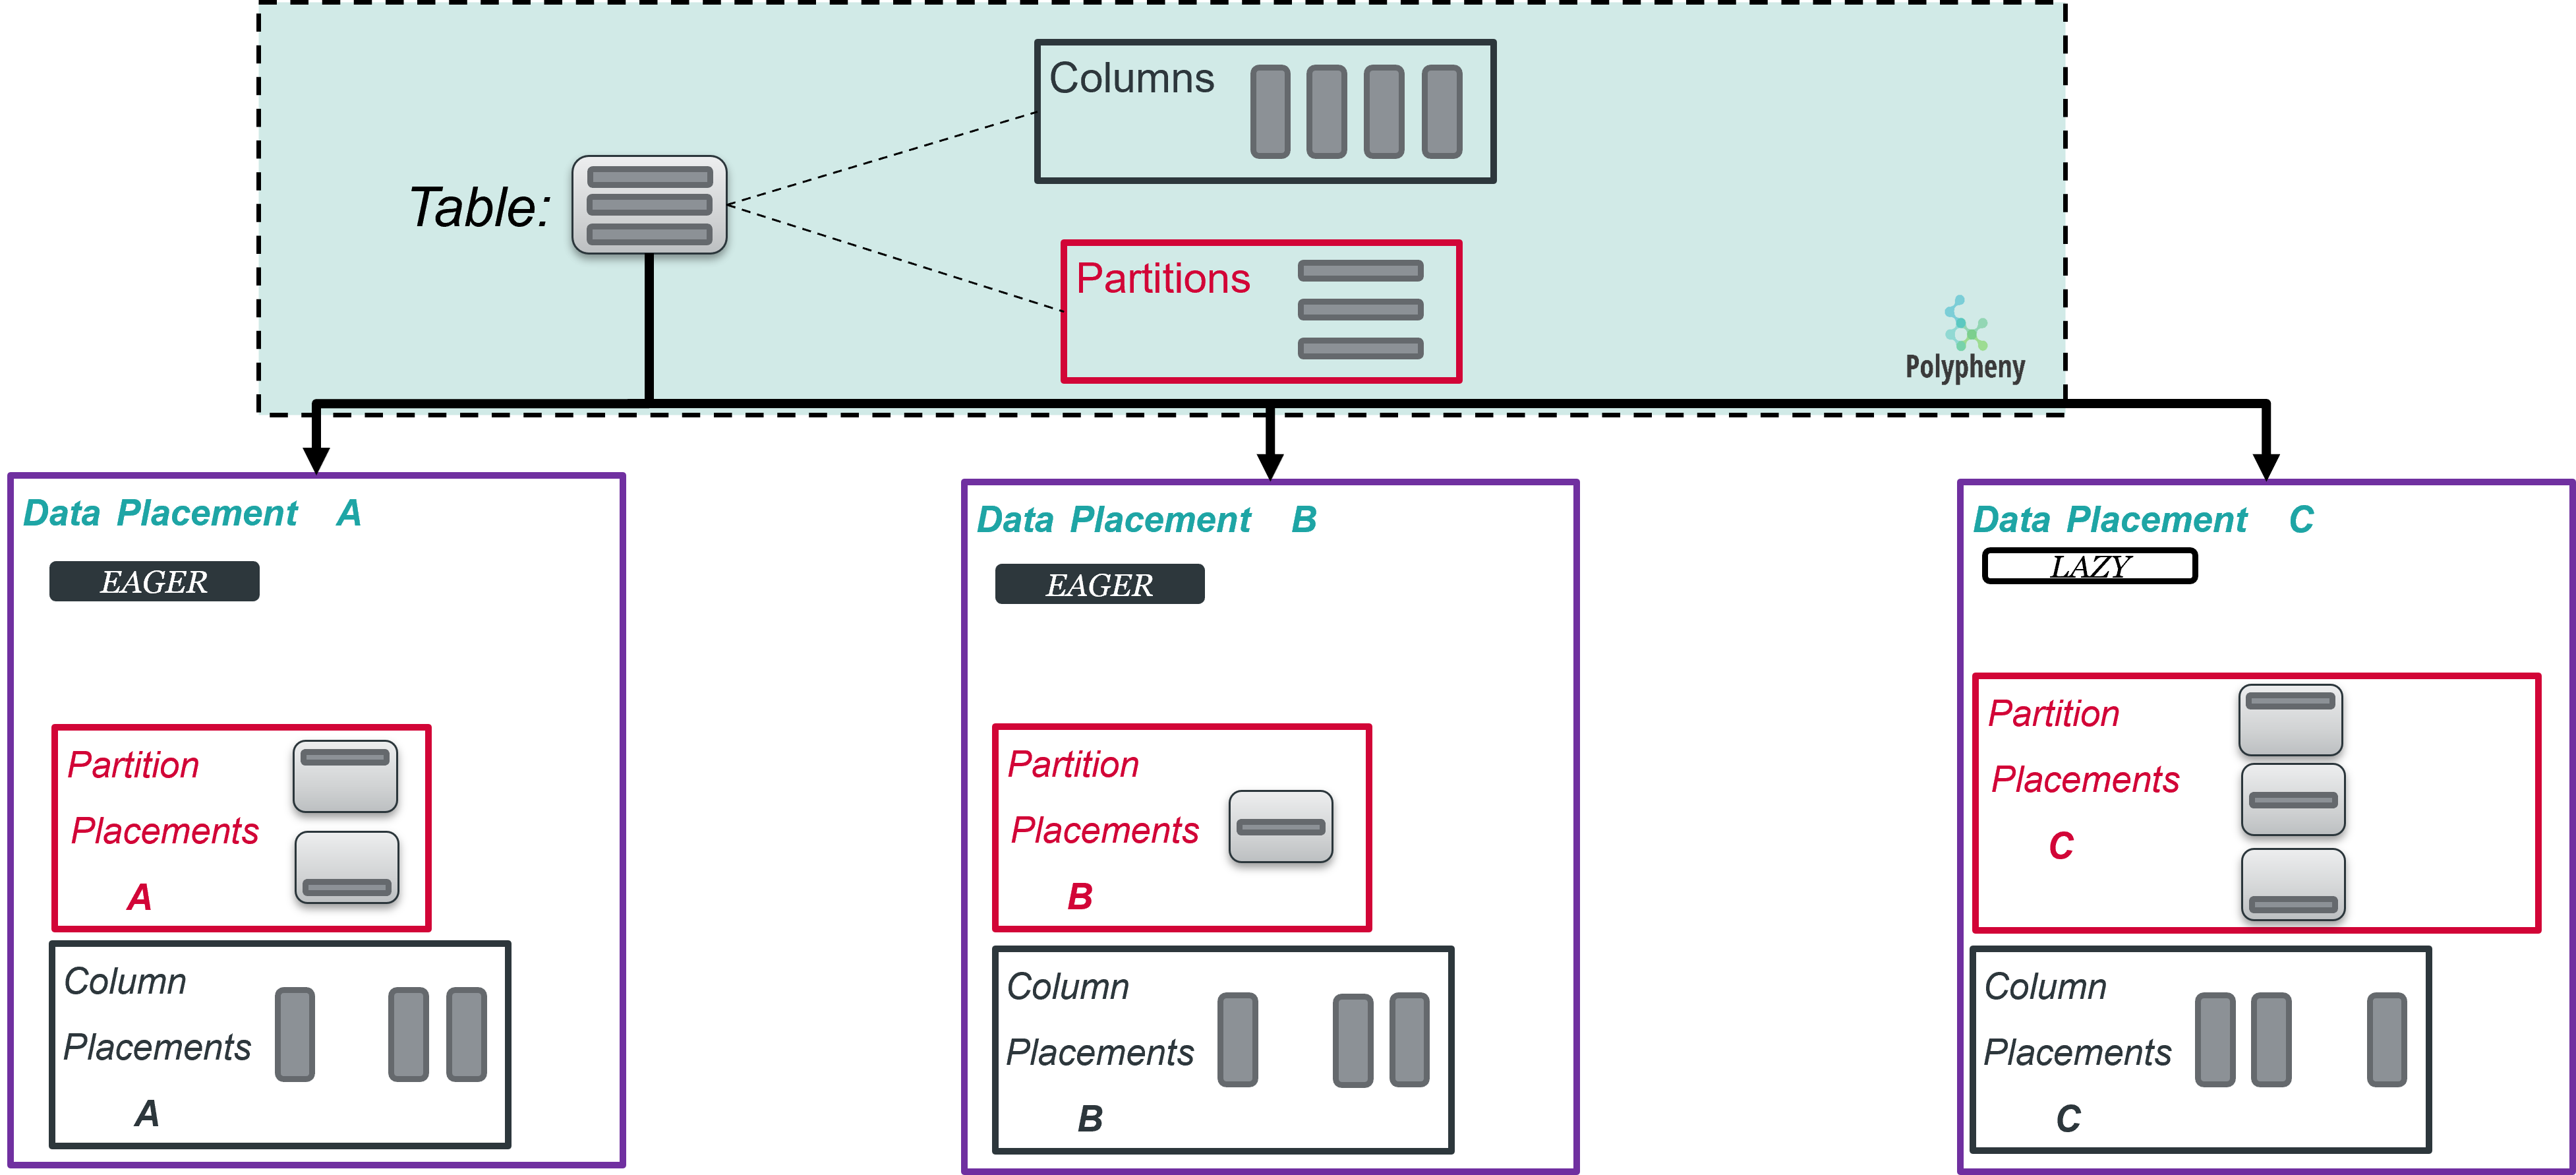
\includegraphics[width=0.7\textwidth]{Figures/entity_placements_replication.png}
    \caption{Entity alongside all its physical placements}
    \label{fig:placements}
\end{figure}



%%%%%%%%%%%%%%%%%%%%%%%%%%%%%%%%%%%%%%%%%%%

\subsection{Replication Strategy}
\label{sec:strategy}

In order to reduce the update time per write-operation and increase the performance
of OLTP workload, we need to enable Polypheny-DB to identify placements that need to receive updates immediately. 

To allow the routing process to differentiate between such placements,
we need the possibility to label data placments on how they are going to receive updates. This is defined as the \emph{Replication Strategy} $\Gamma \in \{EAGER,LAZY\}$.
\emph{EAGER} means that DML operations are applied at once, while \emph{LAZY}
allows data manipulation to be deferred, resulting in outdated data.\\


Although, we defined that we will base the freshness evaluation on partition placements, we implemented the strategy per data placement. 
As introduced in the beginning of this chapter, partition placements inherit their information from its corresponding data placement.
Although they receive there updates independently their properties are defined within the parent placement. 
Therefore, it is sufficient to configure the data placement to achieve an intended state of the subordinate partition placements.
Such that a partition on a given store can either be updated enitrely eagerly or lazily. 

\todoMissing{integrate SYNC and ASYNC}

%Since the locking within Polypheny-DB is done logically within the polystore layer and locks the entire table.
Since we want to establish the freshness comparison on based on each individual partition placement, the locking mechanism
needs to be adapted to allow locking on partition level rather than on a table-level. 


Can be used to selectively define which data placement shall be updated lazily.
The replication strategy can therfore be directly defined as:


\begin{lstlisting}[language=sql]
    ALTER TABLE tableName MODIFY PLACEMENT ON STORE storeName WITH REPLICATION ( LAZY | EAGER );
\end{lstlisting}

This replication strategy is added as part of the newly added data placement properties. Since Data Placements inherently carry the information, what column and partitions reside
on a given store, they were extended to now also hold information on data placement specific properties.


When a placement is created without any replication strategy, it will automatically be labeled to receive updates eagerly.\\
This allows us to flexibly define the strategy per data placement, considering all necessary constraints to ensure the integrity of the data (see \ref{sec:constraints}).


%%%%%%%%%%%%%%%%%%%%%%%%%%%%%%%%%%%%%%%%%%%


\subsection{Replication State}
\label{sec:states}

Since the replication strategy is bound to an individual data placement we still need the possibility to 
define how the actual partition placements, that hold the data, will behave in certain scenarios and will consequently be processed.
We therefore introduce the \emph{Replication State} per partition placement.\\

This replication state is logically bound, and directly influenced by the replication strategy defined within a data placement
and can be differentiated into three states. 
\begin{description}
    \item [UPTODATE] Is automatically set within a partition placement, when the parent placement is configured to receive updates eagerly.
    This cannot be changed by any user. It does also not refer to the current state of any data object, meaning that an lazily updated placement can become up-to-date overtime.
    Allthough this is possible in terms of the received update, it is not respresented using these states. They rather impact the behaviour and handling during processing.
    
    \item [REFRESHABLE] Initially this is configured when the corresponding data placement receives updates lazily. This allows the partition placement to actively receive 
    individual updates by a replication algorithm. A refreshable state can be automatically and manually transformed into an \emph{INFINITELY-OUTDATED} state.

    \item [INFINITELY-OUTDATED] This state is specifically marked, to stay outdated and not receive any updates. This can either be done manually, because a user may want to
    retain an item with a given version, hence surpressing the automatic update replication on this node. Additionally this can be set autoamtically by the system, 
    if either the entire store or the system is not available anymore. This can be caused due to an unexpected outage or simply because the replication algorithm has 
    numerously failed to apply updates, indicating an error. Given certain prerequisites it can be manually transformed back into an \emph{REFRESHABLE} state.

\end{description}

Although, this state is required for internal processing of individual partition placements, the manual specifcation of this state is still targeted to an entire data placement.
Since the internal partitioning should be rathe ruser agnostic one should only be able to specifiy this per data placement. 
As with the replication strategy, the changes are then propagated downwards to all linked partiton placements. 

They have a dependency that refreshable can be set to INFINITELY OUTDAED and vice versa, however UPTODATE can only be influenced by the replicaiton strategy.
Trying to change this manually will result in an error since it is controlled by the system.
\todoMissing{flowchart?}

Placements containing \emph{REFRESHABLE} 

\begin{lstlisting}[language=sql]
    ALTER TABLE tableName MODIFY PLACEMENT ON STORE storeName WITH STATE ( REFRESHABLE | OUTDATED );
\end{lstlisting}
OUTDATED referring to INFINITELY OUTDATED,  by explicitly labeling it as outdated it will suspend all update propagation towards those stores.

Furthermore each Partition Placement is enriched with the most recent update information to support various freshness metrics.
This update information contains insights such as the id of the last comitted update transaction, the corresponding commit and update timestamp as well as the number of 
modifications that 


Therefore, we propose to define the outdatedness on the state of a specific partition placement.
Although the entire data placement, could be labeled as outdated or rather receive updates lazily, some of 
these partitions could already be up-to-date again, while others still remain outdated.




%%%%%%%%%%%%%%%%%%%%%%%%%%%%%%%%%%%%%%%%%%%

\subsection{Lazy Replication Engine}

Is build on a basic \emph{Replication Engine}, that contains the core functionality that transforms capture objects into distinct replication Objects and 
pipes them to specific execution engines.

\todo{add image of global replication Queue}

\begin{description}
    \item[Global Replication Queue] 
    a = defines a unique target placement, 2 the unique replication id and 1000 the associated data id

    \begin{figure}[t]
        \centering
        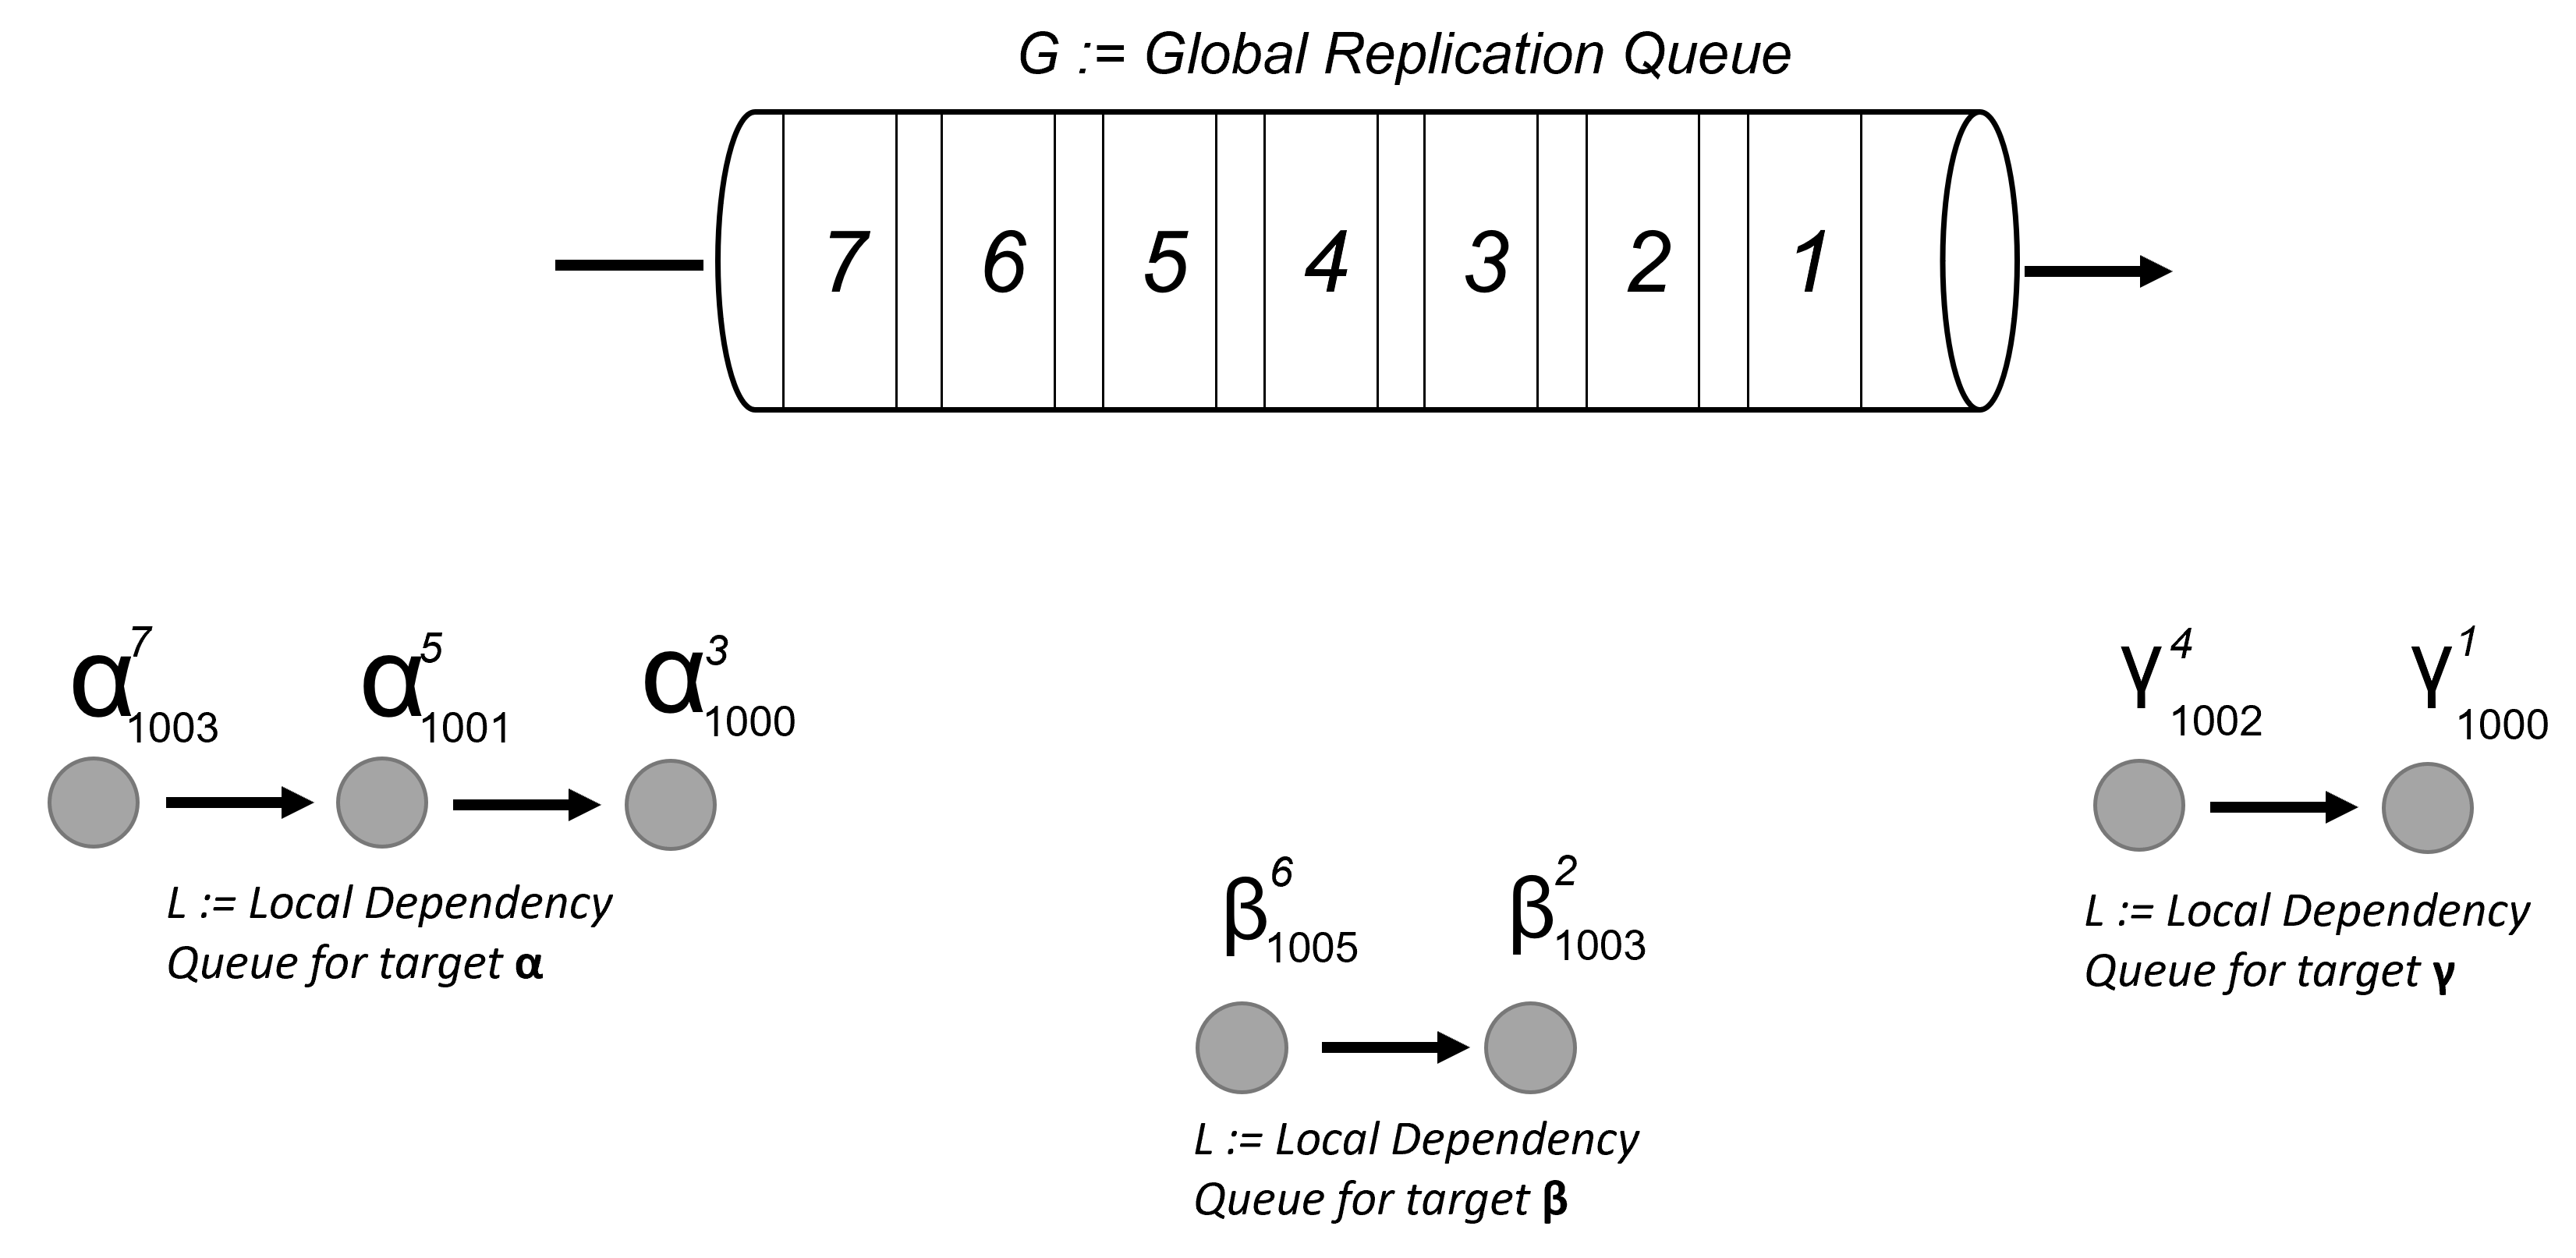
\includegraphics[width=0.8\textwidth]{Figures/Queue.png}
        \caption{Global and local queue}
        \label{fig:queue}
    \end{figure}


    \item[Local Replication Queue]
    \item[Data Replicator]
    \item[Replication Data]
    \item[Replication Worker]
\end{description}


- ReplicationData
- Lazy Execution Workers
- ChangeDataCaptureObject
- ChangeDataCaptureCollectore capture-queue \todo{add picture with statement and transaction id to filter out teh individual capture objects as hashtable }
- Queueing process as flowchart
- replication process as flowchart



\todoMissing{In correspondence to the section \ref{sec:propagation} update propagtion in concept we focussed on implementing the CDC approach ($\rightarrow$ \ref{sec:algo}) 
as well as the on-demand approach using Priamry Snapshot Copy ($\rightarrow$ \ref{sec:manual_refresh}))}

%%%%%%%%%%%%%%%%%%%%%%%%%%%%%%%%%%%%%%%%%%%

\subsection{Automatic Lazy Replication Algorithm}
\label{sec:algo}

\todo{Uses the provided change data capture approach}

The goal of the entire lazy replication approach is providing a scalable and fault tolerant approach to distribute the data for each placement onto the designated stores.
Therefore, the algorithm as depicted in figure \todo{ref image of flowchart}, aims to provide a cost-efficient approach to replicate the change data without increasing the overhead
of the system and impacting the regular operations. 
For every DML-operation the routing process will verify which placements need to receive this modification. During this process, all eagerly replicated stores for this entity
are identified. Since all entities contain a list of all data placements, ergo on which stores this entity has been placed, 
we can compare the delta between the retrieved stores and the actual stores. 
If there is a delta, we can conclude that there are placements which conseqeuntly have to be updated lazily. 
That enabels the entire transaction to \emph{capture change data}. This will directly result in transforming the write-operation into a set of basis operations, 
that are already evaluated and can therefore be immediaetely applied to target placements. Consequently a \emph{Change Data Capture Object} will be created, 
containing all information needed to recreate the statement again. Accompanied with the the ID of the current statement as well as the parent transaction this object is prepared
and appended to the capture-queue.

During runtime when the statement is about to be pushed-down to the designated stores, the prepared statement is enriched with the pre-evaluated information, 
necessary to execute the statement. These parameter values are added to the \emph{Change Data Capture Object} as well. 
Accompanied with the parent transaction and the statement id we can identify this change object within the preliminary capture-queue 
and enrich it with the necessary information (see \todo{add link to image}).\\
As soon as the transaction is finished this object is further processed. If the transaction was aborted and rolledback, we again can directly remove all pre-queued changes 
that are associated with this transaction by removing the entry from the hashtable. This will cascadingly remove all attached capture objects.\\
However, if the transaction will be succesfully commited, the final ization phase starts. For all capture objects associated with this transaction the corresponding commit timestamp of the transaction
will be set. This can later on be used for freshness comparison. Afterwards each capture object will be registered at the \emph{Lazy Replication Engine}. 
To do this, the joint capture object will now be separated into two parts. The first one is the replication data, which contains all information to be applied to 
secondaries as well as all partition placements that shall receive this replication and thus depend on this data. The second one is the creation of independent replication 
objects targeted to individual partition placements. They are bound to a specific operation and responsible for a given target. Additionally they are linked to the single replication Data for this change-data set.
This allows us to reduce the data fottprint by caching the replication data only once. The list of individual replication events as well as the data is now passed on to the
queue registration. This consequently adds for each target placement a new entry into the global queue. Additonally, it also appends the corresponding replication ID to 
the local queue of each partition placement. Once all replication objects have been added to the global queue the finalization phase ends.\\
Since these capture objects have been added to the prelimiary capture-queue in their execution order, they are also passed on to the actual queue in this exact same order.
This ensures the consistency among the different placments, and ensures that they uniformly progress towards a given state as its up-to-date counterpart has.

Since this is all still done before the transaction has publicly finished, further operations are blocked until we have asured that all objects have been consequently transformed and queued within
the associated replication engine. Thus we can ensure the consistency of the secondary placements by waiting until all steps has finished successfully. If something would 
went wrong during queueing, we can still relabel those placments as \emph{INFINITELY OUTDATED}, marking them as not receing any more updates hence informing users and administrators
that this placement will stay outdated until manually fixed.\\

After the queing process has finsihed and the priamry update transaction has returend, removing all locks, the \emph{Replication Workers} will eventually process the queued events.
As soon as a worker has free resources again, it will take the next item out of the global replication queue and starts analyzing it.
For each item it will verify if this is indeed the next replication to be processed for this target, by obtaining the next item of this partition placements local queue.
Additionally it verifies if the replication distribution has been suspended entirely. This will lead the worker to reschedule the replication
and append it at the end of the global queue again, and moving on to the next item.\\
However if this replication does not exist anymore or this target has been marked as \emph{INFINITELY OUTDATED}, avoiding additional replications to be applied,
the worker automatically cleanses the queue from alls remaining replications associated with this placement.\\
Assuming that the currently proccessed event is indded the next replicaiton in line it will prepare the execution and start a new refresh transaction. 
The data replicator will now analyze replication event, and ultiamtely reconstructs a new modification statement that will be routed internally towards the designated partiiton placement.
When the replication has finished the item is removed from the local queue. Additonally it removes itself from the dependency graph of the associated replication data.
If the corresponding replication data does not have any dependencies left, it can also be savely removed to reduce the data footprint of the system again and freeing up resources.
However, if the replication process for this target fails, the centrally defined fail count for this specific replication event is increased. If it is above the configured threhold,
the system will abort further replications of this target placement, labeling it as \emph{INFINITELY OUTDATED} and removing all pending replications of this replica.
Otherwise the replication has been successfully executed.\\


Because the presented lazy update propagation is done operation-wise, we actually loosened the heavy SS2PL constraints that we require on the primary updates. 
Since we already have a serializable schedule after execution, we also know per entity and each partition placement 
the correct execution order that we have to apply the data changes on. So it is not necessary to only free the resources 
after the entire transaction has been replicated but right after each operation. 
However, since Polypheny-DB currently only supports a SS2PL approach we can 
mimic this behaviour by scheduling refresh transaction containing only one modification.
This allows us to replicate using the regualr 2PL approach, hence improving the overall performance of replications with respect to the priamry execution.



\todoMissing{In regards to CDC, if we observe that the number of pending update operations exceed a certain threshold for example 50\% of the total number of modifications of the master
we can directly remove all pending updates and execute a primary snapshot copy because this is faster then reexecuting the operation again. }



\todoMissing{Explain potential optimization steps  that we can analyze the queue and can aggregate certain steps or avoid 
certain operations if we execute batch wise and one UPDATE operation e.g. updates the same primary key}

%%%%%%%%%%%%%%%%%%%%%%%%%%%%%%%%%%%%%%%%%%%

\subsection{Manual Refresh Operations}
\label{sec:manual_refresh}

Despite that the autoamtic refresh operation will take care of most the occuring changes, users might need to be able to specifically priorities certain data placements 
or entire tables to be updated faster than others. This couls also be the case if the placemnt is currently marked as \emph{INFNITELY OUTDATED}
either because of to many failed replications or manually to remain a given state. 
As described in \ref{sec:refresh_operations} we need to be able to provide manual refreshes on the basis of primary snapshot copies.
This inherently uses the capabilities of Poylphenys existing \emph{Data Migrator}, which..
and subsequently will apply this data onto a targeted placement.
This can therefore be used to for snapshot copy.

\todoMissing{Not specifically in manual, altering or inhernetly modifying a data placement with DDLs leaves them as INFINITELY OUTDATED }
\todoMissing{ Or is this automatically detected since we centrally store the replication object and can apply it to arbitrary placements disregarding their local columns or partitions.}

\todoMissing{LazyWorkerThreads - were each worker is responsbile for carrying out one replication or requeing it after it has failed}


%%%%%%%%%%%%%%%%%%%%%%%%%%%%%%%%%%%%%%%%%%%

\subsection{Refresh strategies}
As already stated above, there are essentially three ways to update a secondary node. 
For the automatic execution of propagation transactions a periodic execution has several downsides hence we propose to schedule
refreshment on the basis of the load on the outdated placements. Therefore, we will extend the adapter of the underlying stores to gather metrics on current workload
average response times in order to enable the poly-layer to decide based on this metrics when it is suitable to carry out a propagation-transaction.


Since it might be possible that a user may consider refreshing a placement manually, we have proposed refresh transactions. With this a user has the possibility to refresh
any replicas which are classified as outdated to a specific freshness level.
\begin{verbatim}
ALTER TABLE dummy REFRESH PLACEMENT ON STORE outdated_store 
UNTIL <TIMESTAMP>;
\end{verbatim}
Without any specification the placements shall be updated to the most recent state of the up-to-date version:
\begin{verbatim}
ALTER TABLE dummy REFRESH PLACEMENT ON STORE outdated_store;
\end{verbatim}

For this operation only freshness levels greater than the current local freshness level can be considered.
Furthermore, this should also provide the possibility to refresh all placements of an object.
\begin{verbatim}
ALTER TABLE dummy REFRESH ALL PLACEMENTS;
\end{verbatim}

Although such refresh-transactions can be executed on any placement, it will have no effect on primaries and simply omit their execution. 

%%%%%%%%%%%%%%%%%%%%%%%%%%%%%%%%%%%%%%%%%%%


\todoMissing{ Replication Suspension- Centrally via config for all or specifically for one data placement of a given entity using INFINITELY OUTDATED not to be compaired by a failing placment that is autoamtically marked as INFINITELY outdtaed}

\todoMissing{Resume Distribution - Resumes the distirbution again after it has been centrally suspended}


%%%%%%%%%%%%%%%%%%%%%%%%%%%%%%%%%%%%%%%%%%%

\subsection{Placement Constraints}
\label{sec:constraints}

\todoMissing{What happens for data DDL operations, to they neglect the freshness}

\todoMissing{These changes will also have an impact on the partition distribution constraints. For vertically and horizontally partitioned 
entities this means that all constraints on the number of available column-placements can only be considered for primary update stores. Otherwise, this could harm
the consistency of the system. For nodes labeled as outdated any variation is possible.}

\todoMissing{Maybe outllok adaptively learn the average failcount of certain operations on specific stores to automatically find a good balance between waiting for another try or labeleing it as outdated, therefore a given cost metric would be needed to also ensure 
how often is this outdated palcement even cosnidered in freshness-related queries, do I need it in general }


Furthermore since we are in a distributed setup, we always need to ensure that we do not lose any data, while transforming the indidivdual placements. 
This already starts by defining the replicaiton strategy. Although Polypheny-DB allows to customly distributed an entity across several stores, we have to enforce that no 
information is lost. This means that since we can arbitraly place any combination of columns and partitions of a given entity of any store, we need to make sure that at the end, 
each column is represented by all available partitions at least once. Otherwise ... in violating the integrity of our system. 
This consequently needs to be considered for outdatedness as well. Since we have decoupled updates of eagerly and lazily replicated placements, we again could lose data. 
Therefore we again have to ensure that at least the eagerly replicated placements are sufficently configured such that each column is available for all partitions at least once.
The remaining secondary placements however can again be arbitrarly combined without any requirements.\\
Because it is possible to switch freely between LAZY and EAGER strategies even after tehy contain data, we again have to verify that no data is lost.
Therefore when trying to switch from LAZY to EAGER, we have to ensure that this placement does not contain any pending updates, otherwise the operation will fail.
If there currently are no pending updates the system will lock the entire table, so it will not receive any updates while switching the strategy internally. 
Since this is merely done by setting a flag, the impact of the blocking behaviour can be neglected.\\

Finally, as stated in \ref{sec:states} it is possible to switch the replication states of all partition placements of a given data placement from REFRESHABLE to 
INFINITELY OUTDATED and vice versa.
While the manual switch to INFINITELY OUTDATED is an intentional suspension of the replication procedure, the other direction requires validating possible deviations.
If this is not correctly ensured, and the replication starts propagting changes towards this replication again we will lose data in between on this replica.
In this scenario the system first will need to make sure that the placements on this store are all uptodate. If this is not the case the operation will fail. 
This can be also be done manually by executing a \emph{Primary Snapshot Copy} as described in \ref{sec:manual_refresh}. An immediate chnage of states will then be accepted.



%%%%%%%%%%%%%%%%%%%%%%%%%%%%%%%%%%%%%%%%%%%



\subsection{Placement Refresh}



%%%%%%%%%%%%%%%%%%%%%%%%%%%%%%%%%%%%%%%%%%%%%%%%%%%%%%%%%%%%%%%%%%
%%%%%%%%%%%%%%%%%%%%%%%%%%%%%%%%%%%%%%%%%%%%%%%%%%%%%%%%%%%%%%%%%%
%%%%%%%%%%%%%%%%%%%%%%%%%%%%%%%%%%%%%%%%%%%%%%%%%%%%%%%%%%%%%%%%%%



\section{Freshness Awareness}
This section focusses on all aspects to establish the core aspects of freshness within Polypheny-DB. 


Moreover, to improve the user experience the query tree paths should be extended to specify which level of freshness was requested and with which level it was 
ultimately fulfilled. Furthermore, for successfully executed queries that considered some kind of freshness it shall be added in the SQL response that is has been 
executed by means of a specific freshness level.
In such a way a user can not only steer its desire but is also informed whether the request could be fulfilled.

%%%%%%%%%%%%%%%%%%%%%%%%%%%%%%%%%%%%%%%%%%%

\subsection{Fresnness Evaluation Types}
\todo{maybe put this as description item into another sub section}


%%%%%%%%%%%%%%%%%%%%%%%%%%%%%%%%%%%%%%%%%%%

\subsection{Freshness Query Specification}

This can mainly be achieved by extending the query functionality of Polypheny-DB.
The selection is able to facilitate all possibilities as provided in section 

Although Polypheny-DB provides multiple query interfaces and languages, the following specifications are solely demonstrated with SQL. 
As proposed within section \ref{sec:freshne_metrics} we have introduced essentially three freshness types that can be used to specify a tolerated level of freshness.

Generally all freshness metrics as described in the corresponding sections and along the fucntional requiremnt \textit{(ii)} have also been introduced within Polypheny-DB.

The freshness specification can be appended on any query operation.
For SQL it is extended as an optional leaf expression at the end of every query. 

For the overall freshness guidance an extension of PolySQL is necessary.
Along the description defined users can choose to select any of the specifications to guide the system.
\begin{lstlisting}[language=sql]
SELECT * FROM dummy 
[ WITH FRESHNESS [ <TIMESTAMP> | <DELAY> | <INDEX> ] ];
\end{lstlisting}

Also use simply \emph{WITH FRESHNESS} to specify that you dont care with what freshness it returns


\todoMissing{add this information also at the beginning on lazy replication, when explaining change data capture}
As already described above, we have applied our versioning on the basis of partition placements, since they represent the actual physical tables,
the freshness filtering and evaluation is also always executed by comparing partition placements. 
This is mainly done using metadata within the update information properties of each partition placement. These already contian information on the current commit and update tiemstamp,
the original parent transaction which has updated this placement as well as the numbe rof modifications this particular placement has received.

\todoMissing{relocate to freshness filter inside freshness manager how the filter operations are going to be executed}
For every freshness filter we need to first analyze which partitions are needed for this query. This is done regardless of using freshness or not.
Then the \textit{Freshness Manager} retrieves all available partition palcements for each partition that are lazily replicated.
Afterwards, these lists of partition placements is filtered based on the provided specification.



\begin{description}
    \item[Timestamp] A timestamp is the most simple form of a freshness evaluation type, since it intuitively provides the capability to define 
    an acceptable lower bound of outdatedness, for a specific query. Potential partition placements are therefore filtered by verifying that there commit timestamp is newer
    than the specfied one. Otherwise they are removed from the list of possible candidates.
    
    \item[Time Delay]
    The time delay can be specified together with a time and an associated time unit to define an accetable delay for the desired freshness. 
    This will intuitively substract the specified \emph{absolute time delay} from the current time generating a lower bound timestamp. 
    This again allows filtering all partition placements based on the age of their commit timestamp.
    Again as described in \ref{sec:freshne_metrics}, an absolute time delay based on the current time is not always accurate or might even render wrong results.
    Therefore, a \emph{relative time delay} specification is provided as well. Allowing to specify the tolerated time deviation based on the commit of a priamry placement 
    compared to an outdated placement. To differentiatet those options they are individually suffixed $\in \{ABSOLUTE, DELAY\}$

    \item[Freshness Index]
    Naturally it expresses the freshness specification based on the modification deviation between an up-to-date placement
    and a refreshable placement. The \textbf{Modification Deviation} therefore allows comparing the number of modifications of specific partition placements
    to define a freshness index. For a query this index can be either configured to filter based on each partitions placements deviation or on their accumulated deviation.
    Therefore the number of modifications is accumulated and then compared against the accumultaed number of modifications 
    of all up-to-date entities that have been considered within this query. This allows a more stable approach since it is not prone against outliers. 
    However, this index can also be configured using the freshness index to evaluate the time deviation between two replicas \textbf{Time Deviation}. 
    Essentially the index dictates how accurate a given placement is with respect to its up-to-date replica.
    
\end{description}


After the specification it is enriched 


%%%%%%%%%%%%%%%%%%%%%%%%%%%%%%%%%%%%%%%%%%%

\subsection{Freshness Detection and Extraction}

For every query the query tree is parsed and evaluated in terms of syntactical correctness. Additionally, teh query is analyzed semantically where also the 
freshness will be extracted. This helps to autoamtically enrich the statement with the correct freshness inforamtion and informs the transaction that freshness is being used
which influences locking capabilities and changes the routing process.
The \textit{Freshness Extractor} also checks if for the specified freshness evaluation type

%%%%%%%%%%%%%%%%%%%%%%%%%%%%%%%%%%%%%%%%%%%

\subsection{Freshness Manager}
\todo{Applies filters and combines different possibilities}



\todo{Which possibilities do we have to select a query with freshness}

\todo{How does the freshness respresentation look like for SQL.}

\todoMissing{When a refresh transaction  is executed no more locks on secondary nodes can be applied, if there is still a shared lock on that outdated node
they will first be commited before the refresh takes place  (avoid deadlock) if we do not hinder the system to build more shared locks refresh operations might starve}

\todo{WITH FRESHNESS}
This can be used if a user does not require a minimum level of freshness. This can be easily supported  

%%%%%%%%%%%%%%%%%%%%%%%%%%%%%%%%%%%%%%%%%%%

\subsection{Freshness Filtering}
This is done based on thedifferent freshness evaluation types.


\todo{partition placments are filtered and compared. although as stated in constraints, the priamry and lazy palcement do not have to be equal in terms of there representation (can contian different columns) 
, we therefore just require to compare a partition placement with another eagerly partitoin palcement associated with the same partition.
Allthough the columns good differ, the update and commit is always considered the same since they are based on the same partition. }

%%%%%%%%%%%%%%%%%%%%%%%%%%%%%%%%%%%%%%%%%%%


\subsection{Freshness Selection}
Lifecycle how does the freshness selection process work in geenral. How is filtering combined. 

\todo{State that if no outdated placement can be found we always have the opportunity to fallabck to the master node.}
\todo{Add image}




\todoMissing{The removal of the entity immediately removes all outdated placmenets, so no freshnes or multi version read is possible anymore.
Also if an up-to-date placement is dropped, we need to ensure that we do not lose data otherwise this operation is not possible.}


%%%%%%%%%%%%%%%%%%%%%%%%%%%%%%%%%%%%%%%%%%%
\todo{Maybe not an entire section. Rather discussed internally}
\subsection{Referential Integrity - Freshness Isolation}

\todoMissing{Hence, it might occur that cumulative reads on multiple objects might return incomplete results, since a specified freshness
level can be entirely different on two tables which makes it hard to even compare freshness levels among different objects. However since a user is willing to access 
stale data anyway this is a known risk and thus can be accepted.}

The new isolation level provided by Polypheny-DB in association with freshness can therefore we distinguished between three different levels.
Since we already violated the ACID constraints by returning outdated data, the system initially treats every freshness-related wuery to not acquire any locks on outdated palcements, 
hence allowing dirty reads. This results in refresh operations being able to override or add new results to the placement while it is currently being read. 
While this is not harmful for consecutive write operations that are lazily replicated onto this placement, it could return entirely inconsistent data when 
an \emph{INFINITELY OUTDATED} placement is being refreshed by the data Migrator. Since this empties the table and starts from the beginning. 
Therefore another possibility to avoid those dirty reads is to acquire locks even for outdated or freshness queries. Although the results stay stable and consistent in regards to
the results provided, it will block refresh operations on this placement entirely. Since polypheny-DB uses a version of 2PL shared locks can be easily extended with more transactions adding
itself to the list of waiting transactions, which could lead to starvation of the refresh transaction. Therefore we embedded an extension to this locking approach especially for this use case, which does not interefere with 
the locking mechanism that targets primary copies. When there is currently a shared lock on an object that is about to receive a manual refresh operation, this disables the possibility
for any new upcoming freshness transactions to add itself to the existing shared lock. Instead they are treatetd and added to the dependency graph of the refresh operation (requiring an exclusive lock)
as if they woukd already be an exclusive lock in place. This would avoid straving the refresh operation while still being able to sevre freshness queries on different placements.
This can also be enhanced by centrally configuring \todoMissing{implement} a threshold after how many retries the refresh operation can finally force itself to be executed.
Finally we allow to specify a referential integrity enforcement. As described in section \ref{sec:read_access} we would allow this to try enforcing the referential intergity,
within this transaction. Which also would need to lock the placements. This approach aims to enforce the refernetial intergity among all entitite sused within the transaction.
However in an outdated scenario this can only be ensured if all entities, even have outdated versions of itself and they have all been updated by the same 
transaction and consequently. Otherwise we cannot easily guarantee that they enforce those constraints. If there is doubt or no suitable combination of placements can fulfil this request,
we always have the possibility to fallback to the primary nodes, which are guaranteed to support referential integrity. Allthough, this again blocks updates on the priamry placements,
it fulfils the constriants as it would have when executing the same query without specifying a tolerated level of freshness.

% !TEX root = ../Thesis.tex
\chapter{Evaluation}
\label{c:evaluation}

This chapter is separated into two sections. The first section aims to validate and verify the implementation in terms of their
correct execution. It focuses on the core contributions, such as the lazy replication algorithm as well as the freshness filter capability.
Further it ensures the correct handling of the described constraints and establishes certain test cases to identify possibile failures that can occur 
during execution as well as suitable failure handling scenarios.

The second part of this chapter focuses on benchmarking the implementation on the basis of the individual building blocks itself.
This is followed by comparing the performance of several scenarios to identify how the system will behave in certain situations.
Further it will compare these executions to determine how the implementation fulfils the provided requirements.
Finally the performance of the individual functionalities is benchmarked and compared jointly to give an comprehensive overview on possible performance impacts.


\section{Goal}
The evaluation has three goals: The first goal is to verify the correctness of the solution, the second goal
is identifying the impact freshness-aware aspects have on different workloads and finally the identification of suitable workloads for freshness related queries.

We therefore want to verify and validate the correctness as well as the completeness of the implementation based on several characteristics.
These include the correct execution of the automatic lazy replication procedure, the possibility to refresh statements on demand as well as correct freshness filtering.

Since one of the main goals was to relax the consistency to allow parallel workloads,
we want to identify possible impacts of the replication engine on the overall performance, if freshness indeed increases the possibility
for parallel workload on the system. 
Finally we want to observe if the solution allows harvesting benefits of the underlying stores to adapt to various situations
to assess the benefits of the Polystore in general.
We therefore focus on evaluating the essential functionalities to provide a foundation for future assessments.


%%%%%%%%%%%%%%%%%%%%%%%%%%%%%%%%%%%%%%%%%%%%%%%%%%%%%%%%%%%%%%%%%%

\section{Correctness}
\label{sec:correctness}


The correctness of the introduced solution mainly focuses on two parts. For one the replication behaviour, to verify if each replication is carried out correctly,
and if not verify that reasonable countermeasures are available and apply them. This is crucial since we do not compare the footprint or the integrity of the data after 
a replication update. Rather we compare metadata of two replicas on a high level,
i.e. if the number of modifications and the commit timestamp after the data replication are equal on primary and secondary node. 

The second part of the validation process focuses on the retrieval of outdated nodes. Although we always have the possibility to fallback to the primary placements as described in 
Section \ref{sec:fresh_select}, we still want to avoid excessive locking to parallelize requests to ultimately speed up the average response time.

As mentioned within the implementation chapter, several constraints will already be enforced with the execution itself (see \ref{sec:constraints}). 
We have e.g. established a dependency between the replication strategy as well as the designated placement state. When altering the strategy of an object we
automatically ensure that the state is altered as well. This does not only ensure that the placements will be addressed correctly, but also ensures that no data is lost.
For example it enforces that a lazy replicated placement, that still has pending replications, cannot be switched to now receive updates eagerly.

Furthermore since we have to make sure that no data is lost in general, we have established a strong dependency queue that will apply the update operation-wise in terms of the execution order.
Since we cannot avoid that stores might fail, we have ensured that failing updates will not block the replicaiton queue or will be applied in a wrong order.
Accompanied with a failure-threshols and the placement role \emph{INIFINITELY OUTDATED}, we can instruct the system to mark this placement as permanentely outdated 
avoiding further updates. 
This ensures that all statements labeled as \emph{INIFINITELY OUTDATED} will always be treated correctly.

The freshness specification in general ensures that only acceptable values are considered for the respective evaluation type to propose the correct results and translate it into
a given tolerance value.
Since freshness operations violate the ACID guarantees and we will read stale data, we ensured that these can only be executed within read-only operations, 
such that they do not override data.


Additionally, to guarantee the correctness of the implementation, several unit-tests have 
been created to ensure correct handling of data, when using freshness-awareness or replication approaches in general.
These logically include a purposely false execution of the described constraints to ensure that they will be treated correctly.



%%%%%%%%%%%%%%%%%%%%%%%%%%%%%%%%%%%%%%%%%%%%%%%%%%%%%%%%%%%%%%%%%%

\section{Benchmarks}

The second part of this chapter focuses on the performance impacts of the introduced solutions.
The following steps outline the procedure for benchmarking data freshness within Polypheny-DB.\\
Each evaluation step will subsequently address each required building block to provide data freshness.
Each building block is checked separetely and then put into perspective of the entire context.
These benchmark progressively build on top of each other and are finally summarized with a compound benchmark.\\




\subsection{Evaluation Environment}
\label{sec:env}

For all executed tests a base set of tools n functionality has been used to ensure the reproducibility of the benchmarks.

If not explicitly stated otherwise, the benchmarks will be executed using two underlying stores.
For these stores HSQLDB and PostgreSQL are used. While HSQLDB will run nativiely on the system, PostgreSQL is configured within a virtualized
container environment with limited resources immitating a weaker performing store.
Although not explictly mentioned, each test will always be pre-configured to match the required replication strategy.


%\begin{table}[h]
    %\centering
    %\def\arraystretch{1.5}
    %\begin{tabular}{V{2} l V{2} c|c|c V{2}}
    %\hlineB{3}
    %\textbf{CPU}      & 0       \\ \hline
    %\textbf{RAM}  & 60          \\ \hline
    %\textbf{OS}       & 100     \\ \hline
    %\end{tabular}
    %\caption{Execution Environment Configuration}
    %\label{tab:workload table}
%\end{table}


%docker engine v20.10.11


%\begin{table}[h]
    %\centering
    %\def\arraystretch{1.5}
    %\textbf{DBMS}        & \textbf{#Cores} & \textbf{RAM} & \textbf{Mode}  \\ \hlineB{2}
    %\begin{tabular}{V{2} l V{2} c|c|c V{2}}
    %\hlineB{3}
    %\textbf{HSQLDB}      & 0                 \\ \hline
    %\textbf{PostgreSQL}  & 60        \\ \hline
    %\end{tabular}
    %\caption{Store Configuration for one HSQLDB Store and PostgreSQL Store..}
    %\label{tab:workload table}
%\end{table}





During the evaluation only a predefined set of workloads will be used to obtain insights on various setups.
As suggested in Table \ref{tab:workload table} these inherently differ in terms of their focus on write- or read-operations as well the
degree of utilized freshness queries.\\


\begin{table}[h]
    \centering
    \def\arraystretch{1.5}
    \begin{tabular}{V{2} l V{2} c|c|c V{2}}
    \hlineB{3}
    \textbf{Workload}        & \textbf{Read \%} & \textbf{Write \%} & \textbf{Freshness \%}  \\ \hlineB{2}
    \textbf{Write Only}      & 0                & 100               & 0                             \\ \hline
    \textbf{Mixed Workload}  & 60               & 40         & 0                             \\ \hline
    \textbf{Read Only}       & 100              & 0                 & 0                             \\ \hline
    \textbf{Freshness Only} & 100              & 0                 & 100                           \\ \hline
    \textbf{Mixed Freshness} & 60              & 40                 & 100                           \\ \hline
    \textbf{Partial Freshness} & 100              & 0                 & 50                           \\ \hlineB{2}    
    \end{tabular}
    \caption{Available Benchmark Workloads}
    \label{tab:workload table}
\end{table}



To further assist the execution of the benchmark tests, a number of tools are 
used to standardize and ease the evaluation procedure. These tools are described in the following two sections.

\subsubsection{Chronos}

\textit{Chronos}\footnote{https://chronos-eaas.org/} is a toolkit which enables users to define, 
monitor and analyze the results of an evaluation for several database systems~\cite{vogt_chronos_2020}.
It encompasses several tests and evaluation steps, which will be accumulated in terms of the runtime 
per target. This runtime information can then be used to compare and visualize the differences between different exectution environemnts.  



\subsubsection{OLTPBench}

For all considered functional tests \textit{OLTPBench}\footnote{https://github.com/oltpbenchmark/oltpbench} 
has been used. This benchmarking framework bundles several workload classes and 
encompasses multiple benchmarking tools to seamlessly provide benchmarking for various DBMS~\cite{oltp_2013}.\\
To get a more in-depth view how the implementation affected the overall performance, all tests have been executed 
using \textit{YCSB}\footnote{https://github.com/brianfrankcooper/YCSB}.
\textit{YCSB} not only offers a fundamental correctness test but additionally simulates workload on a single table to obtain essential performance baselines~\cite{ycsb_2010}.
These can be used to retrieve performance metrics and obtain indications regarding correct statement execution and query handling.


%%%%%%%%%%%%%%%%%%%%%%%%%%%%%%%%%%%%%%%%%%%%%%
%%%%%%%%%%%%%%%%%%%%%%%%%%%%%%%%%%%%%%%%%%%%%%

\subsection{Results}
\label{sec:results}
In this section we will present the results of the performance evaluation.
If not stated otherwise the generated tables within the benchmarks will contain 100000 entries and will be executed using
50 parallel client threads on YCSB together with the workloads defined in Table \ref{tab:workload table}.
During the evaluation it will only be referred to the respective workload names.
  

           
\todoMissing{Story - konzept nicht Abstrakt und warum mit Polystore gut - mit Motivation verknüpfen}

\subsubsection{Overhead} 

\begin{figure}[t] 
    \centering 
    \begin{tikzpicture}
        \begin{axis}[
            width  = 0.85*\textwidth,
            height = 7cm,
            x=120pt,
            major x tick style = transparent,
            ybar=.2cm,
            bar width=30pt,
            ymajorgrids = true,
            ylabel = {Runtime (ms)},
            xlabel = {Number of Stores},
            symbolic x coords={1,2},
            xtick = data,
            scaled y ticks = false,
            enlarge x limits=0.40,
            ymin=0,
            major tick style={thick},
            legend pos=outer north east,
            legend cell align=left,
        ]
            \addplot[style={bblue,fill =bblue,mark=none}]
                coordinates {(1, 1454546 ) (2,1712337)};

            \addplot[style={rred,fill=rred,mark=none}]
                coordinates {(1, 1569320) (2,1629462) };

            \legend{Old,New}
        \end{axis}
    \end{tikzpicture}
\caption{Overhead Comparison of Old vs. New Implementation.}
\label{fig:overhead}
\end{figure}

Polystore systems and specifically Polypheny-DB uniformly collect all incoming requests, process them and then
route the resulting queries to the designated stores, where they will be finally executed. 
However, due to this centralized processing, addtional introduced overhead within this layer will directly impact the performance of the system.
Although, Polypheny-DB aims to provide cost- and workload-aware self-adaptiveness, to provide the best possible query results,
its internal processing is executed on top of the actual execution of the underlying store.
This can have a crucial impact on the entire throughput of the system.\\
Hence we used Chronos, a benchmarking tool that allows us to define several evaluation steps per storage engine,
to measure the overhead. For this evaluation the introduced implementation is compared against the current version of Polypheny-DB (v0.7.0).
This was executed using a fixed repeating number of operations, and measured based on the total execution time that it took each configuration
to apply all steps.


As depicted in Figure \ref{fig:overhead}, the results show that the new implementation introduced a little overhead of about 8\% for single store operations.
However with multiple stores the actual execution time was indeed slightly reduced by 5\%. 
Although, single store executions should not be entirely neglected
they do not form the main pursuit of Polystore systems, which are more suitably visualized by the multistore runtime.





%%%%%%%%%%%%%%%%%%%%%%%%%%%%%%%%%%%%%%%%%%%%%%%%%%%%%%%%%%%%%%%%%%

\subsubsection{Locking-Mechanism} 


\begin{figure}[t]
    \centering
    \begin{subfigure}{.5\textwidth}
      \centering
      \begin{tikzpicture}
        \begin{axis}[
            width  = 0.9*\textwidth,
            height=5cm,
            ymajorgrids = true,
            minor y tick num=3,
            ylabel = {Throughput (requests/sec)},
            xlabel = {Number of Partitions ($n$)},
            symbolic x coords={2,4,8},
            xtick = data,
            scaled y ticks = false,
            enlarge x limits=0.40,
            ymin=60,
            ymax=140,
            legend style={
                    at={(1,1.05)},
                    anchor=south east,
                    column sep=1ex
            },
            legend cell align=left,
            smooth
        ]
            \addplot[style={bblue,mark=*}]
                coordinates {(2, 82.66787244) (4,110.0694971) (8,124.4930924)};

            \addplot[style={rred,mark=x}]
                coordinates {(2, 90.32423012) (4,85.38185074) (8,69.04305019)};

            \legend{Single Store,$n$ Stores}
        \end{axis}
    \end{tikzpicture}
      \caption{Old Locking}
      \label{fig:oldlock}
    \end{subfigure}%
    \begin{subfigure}{.5\textwidth}
      \centering
      \begin{tikzpicture}
        \begin{axis}[
            width  = 0.9*\textwidth,
            height=5cm,
            ymajorgrids = true,
            minor y tick num=3,
            ylabel = {Throughput (requests/sec)},
            xlabel = {Number of Partitions ($n$)},
            symbolic x coords={2,4,8},
            xtick = data,
            scaled y ticks = false,
            enlarge x limits=0.40,
            ymin=60,
            ymax=140,
            major tick style={thick},
            legend style={
                    at={(1,1.05)},
                    anchor=south east,
                    column sep=1ex
            },
            legend cell align=left,
            smooth
        ]
            \addplot[style={bblue,mark=square*}]
                coordinates {(2, 83.56813262) (4,118.5016919) (8,136.0429577)};

            \addplot[style={rred,mark=diamond*}]
                coordinates {(2, 75.87686445) (4,90.53951027) (8,68.78432784)};

            \legend{Single Store,$n$ Stores}
        \end{axis}
    \end{tikzpicture}
      \caption{New Locking}
      \label{fig:newlock}
    \end{subfigure}

    \vspace{10pt}%

    \begin{subfigure}{.7\textwidth}
        \centering
        \begin{tikzpicture}
            \begin{axis}[
                width  = 0.7*\textwidth,
                height=5cm,
                ymajorgrids = true,
                ylabel = {Throughput (requests/sec)},
                xlabel = {Number of Partitions ($n$)},
                symbolic x coords={2,4,8},
                xtick = data,
                scaled y ticks = false,
                enlarge x limits=0.40,
                minor y tick num=3,
                ymin=60,
                ymax=140,
                major tick style={very thick},
                legend pos=outer north east,
                legend cell align=left,
                smooth
            ]
                \addplot[style={bblue,mark=*}]
                    coordinates {(2, 82.66787244) (4,110.0694971) (8,124.4930924)};
    
                \addplot[style={rred,mark=square*}]
                    coordinates {(2, 83.56813262) (4,118.5016919) (8,136.0429577)};
    
                \legend{Old,New}
            \end{axis}
        \end{tikzpicture}
        \caption{Old vs. New Locking on a Single Store}
        \label{fig:oldandnewlock}
      \end{subfigure}
    \caption{Impact of Locking Mechanism on the Overall Throughput per Second.}
    \label{fig:lock_comp}
\end{figure}


As described in Section \ref{sec:strategy}, one of the prerequisites to establish multiple refresh strategies and hence lazy replication,  
was the refactoring of the locking mechanism. Although, not completely reworked, the locking-module of Polyphenys SS2PL 
poses as a core component of the system. It therefore impacts correct serializability treatement and is an inherent driver of 
the allowed concurrency which directly influences the overall performance of the system.\\
For the evaluation again the current state of Polypheny-DB is compared against this implementation.
Since the locking module was changed from a table-wise locking towards a partition-wise locking we will validate the impact on the basis of 
a single table using YCSB. 
The evaluation was executed with gradually increasing numbers of partitions, which are placed on one store or distributed across $n$-Stores 
for $n$ partitions to observe any changes on the locking and therefore the throughput.
To get a general overview of the impact, the benchmark was executed using a mixed workload on HSQLDB only.
It is evaluated om the number of operations that can be applied to the system per second.




As visualized in Figure \ref{fig:oldlock} and \ref{fig:newlock}, for both cases the overall situation is quite similiar.
While the distribution of the partitions across several stores gets gradually worse, the single store performance actually improves, the more partitions are added to the table.
This behaviour is essentially caused by Polyphenys need to join and union several stores together, when querying multiple partitions across several stores.
Since more stores need to be connected and considered, it is a rather costly approach and as stated before gets increasingly harder the more stores are involved.

Because the single store variations prove to be more reliable, they are summarized in \ref{fig:oldandnewlock}.
We can observe that the new locking mechanism, indeed proves to be perform around 9\% better in terms of the possible throughput, compared to the old implementation.
Furthermore it shows that again with a growing number of partitions, the gap between the old and new locking extends even more, 
validating the benefits of the new locking mechanism, if used within strongly partitioned configurations.




%%%%%%%%%%%%%%%%%%%%%%%%%%%%%%%%%%%%%%%%%%%%%%%%%%%%%%%%%%%%%%%%%%


\subsubsection{Baseline Identification} 

%%%%%%%%%%%%%%%%%%%%%%%%%%%%%%%%%%%%%%%%%
% Single Store performance of HSQL and PSQL
%%%%%%%%%%%%%%%%%%%%%%%%%%%%%%%%%%%%%%%%%



\begin{figure}[t] 
    \centering 
    \begin{tikzpicture}
        \begin{axis}[
            width  = 0.85*\textwidth,
            height = 6cm,
            x=80pt,
            major x tick style = transparent,
            ybar=.2cm,
            bar width=30pt,
            ymajorgrids = true,
            ylabel = {Avg. Response Time (ms)},
            xlabel = {Stores},
            symbolic x coords={HSQLDB,PostgreSQL},
            xtick = data,
            scaled y ticks = false,
            enlarge x limits=0.50,
            minor y tick num=4,
            ymin=0,
            ymax=3000,
            major tick style={thick},
            legend pos=outer north east,
            legend cell align=left,
        ]
            \addplot[style={bblue,fill=bblue,mark=none}]
                coordinates {(HSQLDB, 2210 ) (PostgreSQL,2700)};

        \end{axis}
    \end{tikzpicture}
    \caption{Distinct Write Time Comparison of HSQLDB and PostgreSQL.}
    \label{fig:singlepsqlhsql}
\end{figure}

The Lazy Replication algorithm is not only fundamental to generate multiple versions to be used within freshness-awareness,
but it is also a core functionality how data is propagated throughout the system. 
Hence, along with the newly introduced replication strategies, and \emph{Change Data Collection} it will have a major impact on the overall perfromance of the system.
Since the replication solely focuses on replicating captured changes, the next benchmarks will be consequently executed using Write Only operations without any reads.


As stated in the evaluation environment \ref{sec:env}, these benchmarks will be mainly executed with an embedded version of HSQLDB and PostgreSQL running within a virtualized 
container environment. To have a general base line for comparison Figure \ref{fig:singlepsqlhsql} presents a single store execution, comparing theses two stores against each other.
As motivated in the beginning, it is crucial for a Polystore system to utilize the key benefits of each store. For our scenario it is therefore, important to determine which 
store configuration is more suitable to be used as an eagerly replicated primary placement, due to its lower latency and better reponse time.\\
This illustrated comparison clearly shows that due to its limited resources the PostgreSQL store
performs on average 22\% slower and cannot directly compete with this HSQLDB store.
This provides us with the intuitive decision to use HSQLDB for the primary transactions.




%%%%%%%%%%%%%%%%%%%%%%%%%%%%%%%%%%%%%%%%%%%%%%%%%%%%%%%%%%%%%%%%%%




\subsubsection{Lazy Replication} 

%%%%%%%%%%%%%%%%%%%%%%%%%%%%%%%%%%%%%%%%%
% Terminal 1 vs. Terminal 50
%%%%%%%%%%%%%%%%%%%%%%%%%%%%%%%%%%%%%%%%%

\begin{figure}[t]
    \centering
    \begin{subfigure}{.5\textwidth}
      \centering
      \begin{tikzpicture}
        \begin{axis}[
            width  = 0.7*\textwidth,
            x=80pt,
            major x tick style = transparent,
            ybar=.2cm,
            bar width=20pt,
            ymajorgrids = true,
            ylabel = {Throughput (requests/sec)},
            xlabel = {Replication Strategy},
            symbolic x coords={Eager,Lazy},
            xtick = data,
            scaled y ticks = false,
            enlarge x limits=0.40,
            ymin=0,
            ymax=30,
            major tick style={thick},
            legend style={
                    at={(1,1.05)},
                    anchor=south east,
                    column sep=1ex
            },
            legend cell align=left,
        ]
            \addplot[style={bblue,fill =bblue,mark=none}]
                coordinates {(Eager, 26.15944582) (Lazy,19.0566423)};

            \addplot[style={rred,fill=rred,mark=none}]
                coordinates {(Eager, 16.9502111) (Lazy,11.78997423) };

            \legend{HSQLDB,PostgreSQL}
        \end{axis}
    \end{tikzpicture}
      \caption{One process}
      \label{fig:terminal1}
    \end{subfigure}%
    \begin{subfigure}{.5\textwidth}
      \centering
      \begin{tikzpicture}
        \begin{axis}[
            width  = 0.7*\textwidth,
            x=80pt,
            major x tick style = transparent,
            ybar=.2cm,
            bar width=20pt,
            ymajorgrids = true,
            ylabel = {Throughput (requests/sec)},
            xlabel = {Replication Strategy},
            symbolic x coords={Eager,Lazy},
            xtick = data,
            scaled y ticks = false,
            enlarge x limits=0.40,
            ymin=0,
            ymax=30,
            major tick style={thick},
            legend style={
                    at={(1,1.05)},
                    anchor=south east,
                    column sep=1ex
            },
            legend cell align=left,
        ]
            \addplot[style={bblue,fill =bblue,mark=none}]
                coordinates {(Eager, 19.08643067 ) (Lazy,14.62659111)};

            \addplot[style={rred,fill=rred,mark=none}]
                coordinates {(Eager, 15.52999761) (Lazy,11.86666016) };
                

                \legend{HSQLDB,PostgreSQL}
        \end{axis}
    \end{tikzpicture}
      \caption{50 processes}
      \label{fig:terminal50}
    \end{subfigure}
    \caption{Throughput Impact of Concurrency in a Replicated Setup.}
    \label{fig:terminal}
\end{figure}

As previously stated, the replication strategies will impact the processing capability of the system immensly.
A placement with a configured lazy replication strategy automatically enables the system, to start tracking changes for this entity, impacting the duration of a query.
Therfore we want to compare how each store handles the replication. Consequently we want to benchmark and compare two equal placements that are eagerly replicated
against the same two stores but one configured as \emph{lazy}.

To extend the baseline discovered before, we again want to demonstrate the behaviour a purely sequential environment with only one client has, 
against a parallel environment with 50 clients.
Figure \ref{fig:terminal} shows the evaluation across two stores, providing the possible throughput per second. This is given as the number of modifications that can be 
applied to the system per second. As before HSQLDB obviously achieves better results then PostgreSQL. Furthermore, disregarding the underlying store,
the eagerly replicated configuration performs much better in all tests, which is not directly apparent when only considering \ref{fig:terminal50}.
However, considering that the collection of changes within a lazy setup, indeed imposes additional costs on the processing time, such deviations are expected.


Admittingly an enitity that is composed of only similiar or equal stores, will not be beneficial for a Polystore system, to allow different workloads.
Therefore the following benchmarks will concentrate on a mixed setup with interleaved stores. These tests will be executed with 50 parallel clients to reproduce a 
conventional environment. 

%%%%%%%%%%%%%%%%%%%%%%%%%%%%%%%%%%%%%%%%%%%%%%%%%%%%%%%%%%%%%%%%%%

%%%%%%%%%%%%%%%%%%%%%%%%%%%%%%%%%%%%%%%%%
% HSQL and PSQL vs. Eager
%%%%%%%%%%%%%%%%%%%%%%%%%%%%%%%%%%%%%%%%%
\subsubsection{Interleaved Configurations}
Now focussing on a mixed setup of two stores containing PostgreSQL as well as HSQLDB for one entity.
Nativiely for a Polystore environment we want to identify which setup of underlying stores will produce better results, hence is suitable for which situation.
Consequently we want to observe how the order of the stores impacts the response time per benchmark.\\
Again to have a foundation to compare our changes to, we will compare the configurations if both stores are defined as eager and Further
respectiviely define each store as lazy as well.\\
Ultimately \ref{fig:psqlhsqlresponse} shows that regarding the lazy approaches, we again see the common behaviour that HSQLDB performs a little better as an eagerly replicated
store compared to PostgreSQL.


\begin{figure}[t] 
    \begin{tikzpicture}
        \begin{axis}[
            width  = 0.9*\textwidth,
            height=6cm,
            ymajorgrids = true,
            ylabel = {Avg. Response Time (ms)},
            xlabel = {Time (sec)},
            scaled y ticks = false,
            minor y tick num=4,
            minor x tick num=9,
            xmin=0,
            xmax=300,
            ymin=2000,
            ymax=5000,
            grid,
            grid style={dotted},
            major tick style={very thick},
            legend style={
                        at={(1,1.05)},
                        anchor=south east,
                        column sep=1ex
                },
            legend cell align=left,
        ]
            \addplot[style={bblue,mark=*}, mark options={scale=0.5}] 
                table [x=time, y=hsql]{Plot/psqlhsqlresponse.dat};
    
            \addplot[style={rred,mark=x}, mark options={scale=0.5}] %[thick]
                table [x=time, y=psql]{Plot/psqlhsqlresponse.dat};
    
            \addplot[style={ppurple,mark=diamond*}, mark options={scale=0.5}] %[thin]
                table [x=time, y=both]{Plot/psqlhsqlresponse.dat};     
    
            \legend{   
                HSQLDB (Eager) - PostgreSQL (Lazy),   
                PostgreSQL (Eager) - HSQLDB (Lazy),           
                PostgreSQL (Eager) - HSQLDB (Eager)
                }
        \end{axis}
    \end{tikzpicture}
    \caption{Response Time Comparsion of Various Store Configurations -- Write Only.}
    \label{fig:psqlhsqlresponse}
    \end{figure}



    \begin{figure}[t] 
        \centering 
        \begin{tikzpicture}
            \begin{axis}[
                width  = 0.7*\textwidth,
                x=80pt,
                major x tick style = transparent,
                ybar=.2cm,
                bar width=20pt,
                ymajorgrids = true,
                ylabel = {Avg. Response Time (ms)},
                xlabel = {Store Compositions},
                symbolic x coords={1},
                xtick = data,
                xticklabels={},
                scaled y ticks = false,
                enlarge x limits=0.40,
                ymin=0,
                ymax=4500,
                minor y tick num=4,
                major tick style={thick},
                legend cell align=left,
                legend pos=outer north east
            ]
                \addplot[style={bblue,fill =bblue,mark=none}]
                    coordinates {(1, 2598.875133)};    
                
                \addplot[style={rred,fill=rred,mark=none}]
                    coordinates {(1, 3194.893767)};    
    
                \addplot[style={ggreen,fill =ggreen,mark=none}]
                    coordinates {(1, 2948.031083)};
    
                \addplot[style={ppurple,fill=ppurple,mark=none}]
                    coordinates {(1, 4018.661833)};
    
                \addplot[style={orange,fill =orange,mark=none}]
                    coordinates {(1, 3475.416683)};
    
                \legend{ 
                    HSQLDB x2 (Eager),
                    PostgreSQL x2 (Eager),
                    PostgreSQL (Eager) - HSQLDB (Eager),
                    PostgreSQL (Eager) - HSQLDB (Lazy), 
                    HSQLDB (Eager) - PostgreSQL (Lazy),
                    }
            \end{axis}
        \end{tikzpicture}
        \caption{Response Time Comparsion of Various Store Compositions -- Write Only.}
        \label{fig:overall_comp}
    \end{figure}


Additionally the Figure in \ref{fig:overall_comp} puts the average latency in perspective to the execution times described before.
As one can observe the eager replications again pefrom the best while the PostgreSQL variation posing as eager, perfroms the worst.
This not only allows to compare the different setups but again aids us to choose suitable store combinations to be used for our designated tasks.\\






%%%%%%%%%%%%%%%%%%%%%%%%%%%%%%%%%%%%%%%%%
% Store Scale 2 vs. 4 HSQL and PSQL
%%%%%%%%%%%%%%%%%%%%%%%%%%%%%%%%%%%%%%%%%

However, the presented possibilities so far only considered the execution on two stores. Therefore, \ref{fig:24storecomp} aims
to compare the execution on two and four stores to identify any deviations the lazy replicaiton algorithm has. 
Again this is done in an interleaved fashion, switching the role of lazy and eager strategy between the participating stores.
During theses tests only one is eagerly replicated, the remaining stores are all configured as lazy placements. Eagerly and lazily replicated stores
in this scenario are defined to be different store types.\\
The graphs indicate that although they differ in terms of average response times, the gap between both configurations is comparably equal.
In both cases the execution with the eagerly replicated HSQLDB is roughly 500ms faster in terms of the average response time.\\

As summarized and visualized more densely in Figure \ref{fig:24storecomp_avg},
its rather counter intuitive that the configurations in \ref{fig:24storecomp} (a) and (b) deviate at all. 
In general they both only contain one primary placement that is even targeted for the primary transaction.
All other stores will be updated asynchronously and are therefore not directly involved.
However, as described before, the primary transaction is also responsible for capturing, as well as queing the changes to be replicated asynchronously.
While the procedure is always executed equally, the second approach with four stores, has more replication targets that require the change. 
Since the generation of replication objects as well as the queueing are all still done during the commit of the primary transaction, the observed
deviations are reasonable.\\

\begin{figure}[t]
    \centering

    \begin{tikzpicture}
        \begin{customlegend}[
            legend columns=2,
            legend style={align=left,column sep=2ex},
            legend entries={HSQLDB (Eager) - PostgreSQL (Lazy),
                            PostgreSQL (Eager) - HSQLDB (Lazy)
                            }]
            \addlegendimage{mark=none,solid,bblue, line legend}
            \addlegendimage{mark=none,rred, solid}   
            \end{customlegend}
        \end{tikzpicture}

        \vspace{10pt}%

    \begin{subfigure}{.5\textwidth}
      \centering
      \begin{tikzpicture}
        \begin{axis}[
            width  = 0.95*\textwidth,
            height=5cm,
            ymajorgrids = true,
            ylabel = {Avg. Response Time (ms)},
            xlabel = {Time (sec)},
            scaled y ticks = false,
            minor y tick num=4,
            minor x tick num=9,
            xmin=0,
            xmax=300,
            ymin=2000,
            ymax=7000,
            grid,
            grid style={dotted},
            major tick style={very thick},
            legend style={
                        at={(1,1.05)},
                        anchor=south east,
                        column sep=1ex,
                        text width=3.5cm
                },
            legend cell align=left,
        ]
            
    
            \addplot[style={bblue,mark=none}, mark options={scale=0.5}] 
            table [x=time, y=hsql_1]{Plot/24storecomp.dat};

            \addplot[style={rred,mark=none}, mark options={scale=0.5}] %[thick]
                table [x=time, y=psql_1]{Plot/24storecomp.dat};      
                %\addlegendentry[minimum height=0.8cm]{HSQLDB (Eager) -\\ PostgreSQL (Lazy)}
                %\addlegendentry[minimum height=1.2cm]{PostgreSQL (Eager) -\\ HSQLDB (Lazy)}
        \end{axis}
    \end{tikzpicture}
      \caption{2 Stores}
      \label{fig:2store}
    \end{subfigure}%
    \begin{subfigure}{.5\textwidth}
      \centering
      \begin{tikzpicture}
        \begin{axis}[
            width  = 0.95*\textwidth,
            height=5cm,
            ymajorgrids = true,
            ylabel = {Avg. Response Time (ms)},
            xlabel = {Time (sec)},
            scaled y ticks = false,
            minor y tick num=4,
            minor x tick num=9,
            xmin=0,
            xmax=300,
            ymin=2000,
            ymax=7000,
            grid,
            grid style={dotted},
            major tick style={very thick},
            legend style={
                        at={(1,1.05)},
                        anchor=south east,
                        column sep=1ex,
                        text width=3.5cm
                },
            legend cell align=left,
        ]
            
    
            \addplot[style={bblue,mark=none}, mark options={scale=0.5}] 
            table [x=time, y=hsql_3]{Plot/24storecomp.dat};

            \addplot[style={rred,mark=none}, mark options={scale=0.5}] %[thick]
                table [x=time, y=psql_3]{Plot/24storecomp.dat};      
    
            %\addlegendentry[minimum height=0.8cm]{HSQLDB (Eager) -\\ PostgreSQL (Lazy) x3}
            %\addlegendentry[minimum height=1.2cm]{PostgreSQL (Eager) -\\ HSQLDB (Lazy) x3}

        \end{axis}
    \end{tikzpicture}
      \caption{4 Stores (Lazy x3)}
      \label{fig:4store}
    \end{subfigure}
    \caption{Response Time Comparison Among Different Store Sizes with Interleaved Roles -- Write Only.}
    \label{fig:24storecomp}
\end{figure}




\begin{figure}[t] 
    \centering 
    \begin{tikzpicture}
        \begin{axis}[
            width  = 0.8*\textwidth,
            height = 6cm,
            x=120pt,
            major x tick style = transparent,
            ybar=.2cm,
            bar width=30pt,
            ymajorgrids = true,
            ylabel = {Avg. Response Time (ms)},
            xlabel = {Number of Stores},
            symbolic x coords={2,4},
            xtick = data,
            scaled y ticks = false,
            enlarge x limits=0.40,
            ymin=0,
            ymax=6000,
            minor y tick num=4,
            major tick style={thick},
            legend style={
                    at={(1,1.05)},
                    anchor=south east,
                    column sep=1ex
            },
            legend cell align=left,
        ]
            \addplot[style={bblue,fill =bblue,mark=none}]
                coordinates {(2, 3653.642433) (4,5346.252567 )};

            \addplot[style={rred,fill=rred,mark=none}]
                coordinates {(2, 4018.661833) (4,5771.588467) };

            \legend{HSQLDB (Eager) - PostgreSQL (Lazy),
                PostgreSQL (Eager) - HSQLDB (Lazy) 
            }
        \end{axis}
    \end{tikzpicture}
    \caption{Avg. Response Time Comparison of Different Store Sizes (4 Stores $\rightarrow$ 1x Eager and 3x Lazy ) -- Write Only.}
    \label{fig:24storecomp_avg}
\end{figure}





%%%%%%%%%%%%%%%%%%%%%%%%%%%%%%%%%%%%%%%%%
% Store Scale 2-8
%%%%%%%%%%%%%%%%%%%%%%%%%%%%%%%%%%%%%%%%%
Based on this observation we specifically wanted to compare how a growth in stores will impact this deviation and how it compares against its eager counterpart. 
To have a more uniform result this test will be executed using only HSQLDB stores, to have a stable foundation for comparison
without a second store that could interfere with the final result.\\
In this evaluation Figure \ref{fig:stores_comp} illustrates, the average response time of two to eight stores, where one store is eagerly replicated and the rest
is configured as lazy.


\begin{figure}[t] 
    \centering 
    \centering
        \begin{tikzpicture}
            \begin{axis}[
                width  = 0.6*\textwidth,
                height = 6cm,
                ymajorgrids = true,
                ylabel = {Avg. Response Time (ms)},
                xlabel = {Number of Stores},
                symbolic x coords={2,4,8},
                xtick = data,
                scaled y ticks = false,
                enlarge x limits=0.40,
                minor y tick num=3,
                ymin=0,
                ymax=6000,
                major tick style={very thick},
                legend pos=outer north east,
                legend cell align=left,
                smooth
            ]
                \addplot[style={bblue,mark=*}]
                    coordinates {(2, 2598.875133) (4,3441.368233) (8,4911.982467)};
    
                \addplot[style={rred,mark=x}]
                    coordinates {(2, 3492.3136) (4,3943.186767) (8,5532.865083)};
    
                \legend{Eager,Lazy}
            \end{axis}
        \end{tikzpicture}
    \caption{Replication Strategy Comparison with Increasing Stores -- Write Only.}
    \label{fig:stores_comp}
\end{figure}

This indicates that although the repsonse time increases, it does so in a stable manner. As compared with its eager approach we can see that it evolves roughly towards the same direction plus the
previously observed offset, generally providing good scalability.

\subsubsection{Queue Replication}

%%%%%%%%%%%%%%%%%%%%%%%%%%%%%%%%%%%%%%%%%
% Single operation comparison
%%%%%%%%%%%%%%%%%%%%%%%%%%%%%%%%%%%%%%%%%

As presented during the implementation and now ellaborated and suggested multiple times during evaluation, 
the capture of modifications to be propagated to the secondary placements, introduces some overhead. Although some overhead
is reasonable due to the additional processing steps, the response times differ 
especially when compared to regular eagerly replicated scenarios. This directly impacts the overall performance,
resulting in generally higher response times for lazy replication scenarios.
Therefore we want to identify for a single write-operation what actually influences these runtime deviations.


\begin{figure}[t] 
    \centering 
    \begin{tikzpicture}
        \begin{axis}[
            width  = 0.8*\textwidth,
            height=6cm,
            ybar stacked,
            x=80pt,
            major x tick style = transparent,
            bar width=30pt,
            ymajorgrids = true,
            ylabel = {Execution Time (ms)},
            xlabel = {Replication Statements},
            symbolic x coords={Eager, Lazy},
            xtick = data,
            scaled y ticks = false,
            enlarge x limits=0.40,
            ymin=0,
            ymax=70,
            minor y tick num=4,
            major tick style={thick},
            legend pos=outer north east,
            legend cell align=left,
        ]
            \addplot+[ybar][style={bblue,fill =bblue,mark=none}]
                coordinates {(Eager, 21) (Lazy, 18)};

            \addplot+[ybar][style={rred,fill=rred,mark=none}]
                coordinates {(Eager, 0) (Lazy, 16)};

            \addplot+[ybar][style={ppurple,fill =ppurple,mark=none}]
                coordinates {(Eager, 0) (Lazy, 28)};

            \legend{ 
                Base Execution,
                Capture Queue,
                Replication,
                }
        \end{axis}
    \end{tikzpicture}
    \caption{Execution Time Comparision of a Decompossed Distinct Write-Operation with and without Active Data Capture.}
    \label{fig:write_decomposition}
\end{figure}



The comparison in Figure \ref{fig:write_decomposition} analyzes the execution time of two independent write operations, respectiviely executed on two equal stores.
One configuration is a simple eager replicated entity on two stores without any replication, the other one is an operation that needs to capture 
the modification within the global replication queue.\\
Since the lazy approach only needs to involve one store for processing, the baseline of the lazy approach is indeed slightly faster than its eager counterpart.
However, considering that at commit time this approach also needs to extract the captured change, convert it into a replication object and ultimately queue 
it for the remaining store, the actual execution deviates quite heavily. With the queue time being almost equal to its the base execution time.\\
However, since the capture part is only executed once at commit time of a transaction, it drastically impacts the performance 
of one single operation.
As we have seen before, this introduced capture gap remains quite stable even with additional targets or capture objects to transform.
Therefore the queueing process negativiely impacts the efficiency for transactions containing only one or few operations.
In contrast it gets neglected further the more operations are actually executed within one transaction.\\
Additionally, although not directly considered to be part of the execution time, is the convergence window. As mentioned before, as soon
as a replication worker will have free resources it will replicate the pending object from the queue onto the secondary store.
As we can see the replication duration actually takes a little bit longer than the actual execution. This is caused by the introduced
validation constraints for each worker to assess the queue and reconstruct each opeartion individually. 
However since the replication is done operation-wise the replication time is considered to be fixed per operation.
Therefore, the entire bar immitates the time it takes for one operation to be executed and replicated across all participating stores,
considering the aforementioned constraints of the queue time.
Since the eagerly replicated approach is executed within one single transaction targeting both underlying stores, the entity is 
considered to be immediately consistent and will not need to converge. 






%%%%%%%%%%%%%%%%%%%%%%%%%%%%%%%%%%%%%%%%%%%%%%%%%%%%%%%%%%%%%%%%%%


\subsubsection{Replica Convergence} 



\begin{figure}[t] 
    \centering 
    \begin{tikzpicture}
        \begin{axis}[
            width  = 0.9*\textwidth,
            height = 7cm,
            x=120pt,
            major x tick style = transparent,
            ybar=.2cm,
            bar width=30pt,
            ymajorgrids = true,
            ylabel = {Execution Time (sec)},
            xlabel = {Number of Stores},
            symbolic x coords={2,4},
            xtick = data,
            scaled y ticks = false,
            enlarge x limits=0.40,
            ymin=0,
            ymax=45,
            minor y tick num=4,
            major tick style={thick},
            legend style={
                    at={(1,1.05)},
                    anchor=south east,
                    column sep=1ex
            },
            legend cell align=left,
        ]
            \addplot[style={bblue,fill =bblue,mark=none}]
                coordinates {(2, 33.4120) (4,39.18 )};

            \addplot[style={rred,fill=rred,mark=none}]
                coordinates {(2, 30.322) (4,36.9) };

            \legend{HSQLDB (Eager) - PostgreSQL (Lazy),
                PostgreSQL (Eager) - HSQLDB (Lazy) 
            }
        \end{axis}
    \end{tikzpicture}
    \caption{Convergence Time Comparison on Different Store Constellations and Sizes (4 Stores $\rightarrow$ 1x Eager and 3x Lazy ) -- Mixed Workload.}
    \label{fig:store_comparision}
\end{figure}

As we have seen before the versions can deviate quite heavily during a mixed workload. 
Furthermore, we have already identified that configuring the faster perfoming store to be replicate eagerly, proofs that this will positiviely impact 
the availability due to its lower repsonse time of the inital transaction.
However as important as the throughput of initial transaction might be, choosing the faster node to be eagerly replicated intuitively leaves the slower node
to apply the updates asynchronously. 
However, because it highly depends on the requirements which configuration to choose, we also want to establish a setup that focuses on quickly reaching
a consistent state without using an eager-only replication setup.



Therefore, we want to observe the actual replication time until two stores reach an equilibrium in terms of their received updates.\\
The plot in \ref{fig:store_comparision} visualizes the comparison based on a different number of stores.

Due to the fact that HSQLDB was before identifed as the store with the better throughput, 
it also generally manages to converge faster if configured to be the secondary store. 
Since HSQLDB in our scenario is able to replicate the operations faster than the primary transaction can queue new events,
it does not only converge faster but has a lower execution time in general.\\
Therefore we have established that with our introduced algorithm, indeed
the better performing store is also more suitable when we want to reach consistency faster, hence providing a smaller convergence time.\\




Although that the convergence time is not essentially impacted by the executing store, but also by the number of designated stores that shall asynchronously 
receive the operation. 
Further we want to identify how the queue behaves if the secondary system is generally slower and therefore not able to replicate 
the pending changes as fast as new ones are added to the queue.



  \begin{figure}[t]
    \centering

    \begin{tikzpicture}
        \begin{customlegend}[
            legend columns=2,
            legend style={align=left,column sep=2ex},
            legend entries={Response Time (ms),
                            Replication Queue
                            }]
            \addlegendimage{mark=none,solid,bblue, line legend}
            \addlegendimage{mark=none,rred, solid}   
            \end{customlegend}
        \end{tikzpicture}

    \begin{subfigure}{.5\textwidth}
      \centering
      
        \begin{tikzpicture}
        \begin{axis}[
            scale only axis,
            width  = 0.6*\textwidth,
            axis y line*=left,% the ’*’ avoids arrow heads
            height=3cm,
            ylabel = {Avg. Response Time (ms)},
            xlabel = {Time (sec)},
            scaled y ticks = false,
            minor y tick num=4,
            minor x tick num=4,
            xmin=0,
            xmax=340,
            ymin=2000,
            ymax=6000,
            ylabel shift=-4pt,
            restrict x to domain=0:305,
            grid,
            grid style={dotted},
            major tick style={very thick},
            legend style={
                            at={(1,1.05)},
                            anchor=south east,
                            column sep=1ex
                    },
            legend cell align=left,
        ]
        \addplot[style={bblue,mark=none}, mark options={scale=0.5}] 
                    table [x=time, y=psql_1]{Plot/converge24.dat};
            
        \end{axis}
        \begin{axis}[
            scale only axis,
            width  = 0.6*\textwidth,
            height=3cm,
            xmin=0,
            xmax=340,
            ylabel shift = -4pt,
            ymin=0,
            ymax=800,
            axis y line*=right,
            axis x line=none,
            ylabel=Queue Size
          ]
          \addplot[style={rred, fill=rred, fill opacity=0.4, mark=none}, mark options={scale=0.5}] %[thick]
                    table [x=time, y=queue_2]{Plot/converge24.dat};
        \end{axis}
      \end{tikzpicture} 
      \caption{2 Stores}
      \label{fig:converge_2}
    \end{subfigure}\hfill% 
    \begin{subfigure}{.5\textwidth}
      \centering
      \begin{tikzpicture}
        \begin{axis}[
            scale only axis,
            width  = 0.6*\textwidth,
            height=3cm,
            axis y line*=left,% the ’*’ avoids arrow heads
            ylabel = {Avg. Response Time (ms)},
            xlabel = {Time (sec)},
            scaled y ticks = false,
            minor y tick num=4,
            minor x tick num=4,
            xmin=0,
            xmax=405,
            ylabel shift=-4pt,
            ymin=2000,
            ymax=6000,
            restrict x to domain=0:310,
            grid,
            grid style={dotted},
            major tick style={very thick},
        ]
        \addplot[style={bblue,mark=none}, mark options={scale=0.5}] 
                    table [x=time, y=psql_3]{Plot/converge24.dat};
                
        \end{axis}
        \begin{axis}[
            scale only axis,
            width  = 0.6*\textwidth,
            height=3cm,
            xmin=0,
            xmax=405,
            ymin=0,
            ymax=4000,
            ylabel shift = -4pt,
            axis y line*=right,
            axis x line=none,
            ylabel=Queue Size
          ]
          \addplot[style={rred, fill=rred, fill opacity=0.4, mark=none}, mark options={scale=0.5}] %[thick]
                    table [x=time, y=queue_4]{Plot/converge24.dat};

        \end{axis}
      \end{tikzpicture}
      \caption{4 Stores}
      \label{fig:converge_4}
    \end{subfigure}
    \caption{Execution Time along the Replication Queue Convergence -- Mixed Workload.}
    \label{fig:converge_24}
\end{figure}



%%%% %% %%

For this test we are using a Mixed Workload to allow permanent access to the primary node (HSQLDB), while the lazy replicated nodes (PostgreSQL) can solely concentrate on applying the queued changes.
Figure \ref{fig:converge_24} visualizes the expansion- as well as the shrinking-phase of the replication queue
and puts it into perspective along with the actual test execution. During these tests one worker continuously processed the queue and replicated 
the changes operation-wise. As illustrated in both cases the worker is not able to apply the changes faster than they are coming in.
The breakeven point is reached as soon as the test execution has finished and the load on the system stops. For both configurations the algorithm can now quickly propagate all pending
changes.
Certainly this is caused by the different performance capabilities of the underlying stores. 
While HSQLDB as a lazy replicated store can process and apply the events faster, 
leaving the queue mostly empty, PostgreSQL is not able to match this performance applying the replication events slower than new ones
are generated. This then causes the queue to grow until there is no more load on the system.
Without a defined test enviornemnt in regular situations with continous load, this could cause severe problems,
since the queue will grow without bound.

\begin{figure}[t] 
    \centering 
    \begin{tikzpicture}
        \begin{axis}[
            width  = 0.8*\textwidth,
            height=5cm,
            ymajorgrids = true,
            ylabel = {Queue Size},
            xlabel = {Time (sec)},
            scaled y ticks = false,
            minor y tick num=4,
            minor x tick num=4,
            xmin=0,
            xmax=405,
            ymin=0,
            ymax=4000,
            grid,
            grid style={dotted},
            major tick style={very thick},
            legend pos=outer north east,
            legend cell align=left, 
        ]
            \addplot[style={bblue, fill=bblue, fill opacity=0.6, mark=none}, mark options={scale=0.5}] 
                table [x=time, y=queue_2]{Plot/converge24.dat};
    
            \addplot[style={rred, fill=rred, fill opacity=0.4, mark=none}, mark options={scale=0.5}] %[thick]
                table [x=time, y=queue_4]{Plot/converge24.dat};
      
    
            \legend{   
                2 Stores,   
                4 Stores
                }
        \end{axis}
    \end{tikzpicture}
    \caption{Replication Queue Convergence Over Time -- Mixed Workload.}
    \label{fig:converge24}
\end{figure}


Because captured change operations are also transformed $1-n$ for $n$ lazy replicated stores, the size of the queues is essentially influenced by the number of replicas that
require the change. 
As summarized in Figure \ref{fig:converge24} this directly influences the earlier described convergence time of our system and negativiely impacts the response time.
Which makes the selected storage constellation crucial.









%%%%%%%%%%%%%%%%%%%%%%%%%%%%%%%%%%%%%%%%%%%%%%%%%%%%%%%%%%%%%%%%%%
\subsubsection{Freshness Evaluation Type Filter} 

The benchmarks so far merely focussed on the replication as well as the write operations.
Therefore the next evaluations will concentrate on testing the introduced freshness capabilities.

Despite the actual usage of freshness operations in general, also the chosen evaluation type will influence the performance.
Although, that the filter comparison itself is always executed equally, the filter generation can differ between the available types.

\begin{figure}[t] 
    \centering 
    \begin{tikzpicture}
        \begin{axis}[
            width  = 0.8*\textwidth,
            height=6cm,
            x=80pt,
            major x tick style = transparent,
            ybar=.2cm,
            bar width=25pt,
            ymajorgrids = true,
            ylabel = {Avg. Response Time (ms)},
            xlabel = {Evaluation Types},
            symbolic x coords={1},
            xtick = data,
            xticklabels={},
            scaled y ticks = false,
            enlarge x limits=0.40,
            ymin=0,
            ymax=3500,
            minor y tick num=4,
            major tick style={thick},
            legend pos=outer north east,
            legend cell align=left,
        ]
            \addplot[style={bblue,fill =bblue,mark=none}]
                coordinates {(1, 3000)};

            \addplot[style={rred,fill=rred,mark=none}]
                coordinates {(1, 3190)};

            \addplot[style={ggreen,fill =ggreen,mark=none}]
                coordinates {(1, 3350)};

            \addplot[style={ppurple,fill=ppurple,mark=none}]
                coordinates {(1, 3150)};

            \legend{ 
                Timestamp,
                Absolute Delay,
                Relative Delay,
                Freshness Index
                }
        \end{axis}
    \end{tikzpicture}
    \caption{Avg. Response Time Comparison of Available Evaluation Types -- Freshness Only}
    \label{fig:eval_type}
\end{figure}

While a timestamp can be directly used as it is, an index first needs to aggregate the total number of modifications per placement and 
calculate the comparison-index based on the deviation from the master.
Albeit, that this is not a very costly operation, it will have a significant impact when executed multiple times.
To obtain comparable results, the benchmarks have been executed with the most liberal degree of freshness per type, to avoid any side affects or fallbacks to the primary nodes.\\
Figure \ref{fig:eval_type} therefore presents the overall latency of a mixed workload accompanied by the different evaluation types.
As already suggested all types provide a very similar response time. A difference becomes only really obvious when e.g. comparing a natively usable
timestamp to a relative time delay. While the first one can be applied directly the later first
needs to extract the commit time of all possible placments and apply the deviation before it is actually able to filter.
This plot shows that although only marginally different the utilized filter will still slightly impact the overall performance.




%%%%%%%%%%%%%%%%%%%%%%%%%%%%%%%%%%%%%%%%%%%%%%%%%%%%%%%%%%%%%%%%%%

\subsubsection{Freshness-Aware Read Operations}

As with write only operations also the freshness can directly indicate a suitable store combination.
While write-operations focus on a trade-off between latency of the primary transaction and a faster convergence time,
the read-operations will consequently focus on the target where the read is applied. While regular read-operations exclusively target
primary placements, freshness-queries will mainly be redirected towards possibly outdated secondary replicas.


As described before, since freshness related results are essentially influenced by the entity composition, we need an independent measurement.
Therefore we will  compare two equal stores (HSQLDB) to again allow a base comparison and observe how the freshness specification itself impacts the results.


\begin{figure}[t] 
    \centering 
    \begin{tikzpicture}
        \begin{axis}[
            width  = 0.9*\textwidth,
            height=6cm,
            ymajorgrids = true,
            ylabel = {Avg. Response Time (ms)},
            xlabel = {Time (sec)},
            scaled y ticks = false,
            minor y tick num=4,
            minor x tick num=9,
            xmin=0,
            xmax=300,
            ymin=0,
            ymax=2500,
            grid,
            grid style={dotted},
            major tick style={very thick},
            legend style={
                        at={(1,1.05)},
                        anchor=south east,
                        column sep=1ex
                },
            legend cell align=left,
        ]
            
    
            \addplot[style={bblue,mark=*}, mark options={scale=0.5}] 
            table [x=time, y=100]{Plot/fresh0.dat};

            \addplot[style={rred,mark=x}, mark options={scale=0.5}] %[thick]
                table [x=time, y=50]{Plot/fresh0.dat};      
            
            \addplot[style={ppurple,mark=diamond*}, mark options={scale=0.5}]% [thin]
                table [x=time, y=both]{Plot/fresh0.dat};  
    
            \legend{  
                100\% Freshness, 
                50\% Freshness,
                0\% Freshness   
                }
        \end{axis}
    \end{tikzpicture}
    \caption{Response Time Comparision on Varying Proportions of Freshness.}
    \label{fig:fresh0}
\end{figure}



Therefore \ref{fig:fresh0} shows a comparison of different degrees of freshness used within a pure read-only environement.
These results generally show that the utilized freshness alone is already sufficient to provide better read results than if no freshness is used at all.
As before this is inherently caused by the targeted store of the query. While all queries without a freshness specification will directly contact a primary node,
hence needing to apply a lock, freshness queries can contact the secondary node without a lock. Although in general shared-locks can be easily applied for regular read-operations, they still need to be formally acquired impacting
the throughput. The most benefit can therefore be gained by combining the freshness with regular operations. As depicted above, these combinations provide by far 
the best results. Despite that regular reads still need to acquire a lock, these different query types will consequently also target different stores. 
This allows an efficient load distribution across the utilized stores, to harvest the benefits of a distributed environement increasing the overall throughput.




Even with a mixed workload without any freshness constraints we already observed that the store constellation does have an impact on the overall latency 
and influences the decission process. 
These effects can also be considered when evaluating a partial workload on our interleaved setup with HSQLDB and PostgreSQL.


\begin{figure}[t] 
    \centering 
    \begin{tikzpicture}
        \begin{axis}[
            width  = 0.9*\textwidth,
            height = 7cm,
            x=120pt,
            major x tick style = transparent,
            ybar=.2cm,
            bar width=30pt,
            ymajorgrids = true,
            ylabel = {Avg. Response Time (ms)},
            xlabel = {Freshness Degree},
            symbolic x coords={0\%,100\%},
            xtick = data,
            scaled y ticks = false,
            enlarge x limits=0.40,
            ymin=0,
            ymax=4000,
            minor y tick num=4,
            major tick style={thick},
            legend style={
                    at={(1,1.05)},
                    anchor=south east,
                    column sep=1ex
            },
            legend cell align=left,
        ]
            \addplot[style={bblue,fill =bblue,mark=none}]
                coordinates {(0\%, 2504.659922) (100\%,3050 )};

            \addplot[style={rred,fill=rred,mark=none}]
                coordinates {(0\%, 2620) (100\%,2856.9465) };

            \legend{HSQLDB (Eager) - PostgreSQL (Lazy),
                PostgreSQL (Eager) - HSQLDB (Lazy) 
            }
        \end{axis}
    \end{tikzpicture}
    \caption{Impact of Store Selection based on Varying Proportions of Freshness -- Partial Freshness.}
    \label{fig:mixed}
\end{figure}

The illustration in \ref{fig:mixed}, therefore indicates the impact a given store constellation has on the overall throughput.
While regular operations perform better in the configuration targeting HSQLDB as the priamry node,
whereas queries with freshness, target the secondary node essentially flipping the roles.
This is again caused by the target of the select statements. 
Since we are rather in a read-heavy environemnt the selection has quite the impact on the final result.
This proves that the store consteallation will strongly influence the systems behaviour as well as the designated workloads to use this constellation on.


%%%%%%%%%%%%%%%%%%%%%%%%%%%%%%%%%%%%%%%%%%%%%%%%%%%%%%%%%%%%%%%%%%
\subsubsection{Compound Operations} 

Now with every building block evaluated independently, we will combine and assess the given funcitonality jointly.


%%%%%%%%%%%%%%%%%%%%%%%%%%%%%%%%%%%%%%%%%
% Mixed with Freshness comparison
%%%%%%%%%%%%%%%%%%%%%%%%%%%%%%%%%%%%%%%%%

Based on the elementary comparison in Figure \ref{fig:write_decomposition} we have already established the heavy impact the capture-queue as well as the 
replication have on a single write-operation.

As mentioned in the implementation, depending on the current load on the system, we might observe contentions since the replication is done in parallel.
Furthremore we might even come across situations where an administrator will directly define a placement as \emph{INFINITELY OUTDATED} to not receive any more updates
and retain its current version.\\
For the next benchmark we therefore want to see how the workload behaves if the replicaton is done in parallel, if the replication distribution is suspeneded
and if the entire queue-capture is suspended.
This is again done using two HSQLDB stores, to reduce possible deviations across stores. 
Additionally this benchmark introduces freshness queries, to observe how it influences the overall response time even when there is no active replication. 
The freshness evaluation utilizes a freshness-index of $0.7$ to filter and identify possible candidates based on the number of received modifications.


\begin{figure}[t] 
    \centering 
    \begin{tikzpicture}
        \begin{axis}[
            width  = 0.9*\textwidth,
            height=6cm,
            ymajorgrids = true,
            ylabel = {Avg. Response Time (ms)},
            xlabel = {Time (sec)},
            scaled y ticks = false,
            minor y tick num=4,
            minor x tick num=9,
            xmin=0,
            xmax=300,
            ymin=0,
            ymax=7000,
            grid,
            grid style={dotted},
            major tick style={very thick},
            legend style={
                        at={(1,1.05)},
                        anchor=south east,
                        column sep=1ex
                },
            legend cell align=left,
        ]
            
    
            \addplot[style={bblue,mark=*}, mark options={scale=0.5}] 
            table [x=time, y=active]{Plot/replication_impact.dat};

            \addplot[style={rred,mark=x}, mark options={scale=0.5}] %[thick]
                table [x=time, y=replication]{Plot/replication_impact.dat};      
            
            \addplot[style={ppurple,mark=diamond*}, mark options={scale=0.5}]% [thin]
                table [x=time, y=capture]{Plot/replication_impact.dat};  
    
            \legend{  
                Replication Active,
                Replication Suspended,
                Capture + Replication Suspended,
                }
        \end{axis}
    \end{tikzpicture}
    \caption{Impact of Replication Queue on Response Time using Freshness (Index=0.7) -- Partial Freshness.}
    \label{fig:replication_impact}
\end{figure}

As provided by Figure \ref{fig:replication_impact} we can again observe that the overall response time improves if there is no active replication running in the background.
Furthermore, the system performs best if it does not need to capture any changes at all, 
which essentially corresponds to the observations we have described in Figure \ref{fig:write_decomposition}.
Although this is rather a corner case, the replication suspension on the other hand is more likely to occur and still provide good response times.

Interestingly, we further observe peaks on the active replication graph. While the graphs without replication and capture mechanisms are more narrow,
the active replication queue oscilates quite heavily, negativiely impacting the average response time.\\
Further, we observe that these peaks start occuring after roughly one minute.
Since we used a modification deviation for our freshness specification, the system is able to quickly identify suitable placements in the beginning of the benchmark.
However, after some time the versions start deviating quite heavily from its eager version.
Since the updates are only propagated operation-wise, and the replications cannot catch up with the primary operations anymore as already presented in Figure \refname{fig:converge24}.
Hence the system is not able to fulfil the tolerated freshness-level and
causes the algorithm to fall back to its primary placement, again investing additional time to combine and select a suitable combination of placements, which ultimately causes the peaks.




%%%%%%%%%%%%%%%%%%%%%%%%%%%%%%%%%%%%%%%%%
% Partition
%%%%%%%%%%%%%%%%%%%%%%%%%%%%%%%%%%%%%%%%%
\subsubsection{Partitioning} 

Our freshness and replication implementation essentially revolves around the handling of individual Partition Placements.
However, so far all tests only really considered unpartitioned entities to visualize basic differences. 

\begin{figure}[t] 
    \centering 
    \begin{tikzpicture}
    \begin{axis}[
        width  = 0.8*\textwidth,
        height=6cm,
        x=80pt,
        major x tick style = transparent,
        ybar=.2cm,
        bar width=25pt,
        ymajorgrids = true,
        ylabel = {Avg. Response Time (ms)},
        xlabel = {Partition Constellations},
        symbolic x coords={1},
        xtick = data,
        xticklabels={},
        scaled y ticks = false,
        enlarge x limits=0.40,
        ymin=0,
        ymax=3000,
        minor y tick num=4,
        major tick style={thick},
        legend pos=outer north east,
        legend cell align=left,
    ]
        \addplot[style={bblue,fill =bblue,mark=none}]
            coordinates {(1, 444.19055)};

        \addplot[style={rred,fill=rred,mark=none}]
            coordinates {(1, 364)};

        \addplot[style={ggreen,fill =ggreen,mark=none}]
            coordinates {(1, 2395)};

        \legend{ 
            5 Stores - 4 Partitions,
            2 Stores - 4 Partitions,
            2 Stores - Unpartitioned
            }
    \end{axis}
\end{tikzpicture}
    \caption{Impact of Partitioning on Freshness (Index=0.7), Across Lazy Replicated Stores -- Partial Freshness.}
    \label{fig:partition_result}
\end{figure}

Accompanied with the introduced locking changes and the promising results described in Figure \ref{fig:lock_comp}, we will evaluate the Partial Freshness workload in 
a partitioned environement. For one we will partition the table into four horizontal partitions. 
For one scenario we place all partitions on the eager node and then each partition respectiviely on four lazy replicated stores to achieve a highly distributed setup as before.
The second scenario will place all four partitions across two stores, where exactly one is eagerly and the other lazily replicated. 
These two variations are ultimately compared against an entire unpartitioned setup across two HSQLDB stores which is visualized in Figure \ref{fig:partition_result}.


Analogously, to the results obtained from the locking mechanism benchmarks, 
these results consequently indicate, that we achieve the best performance
if we indeed partition the entity and place all partitions on each entity across both stores. This natively allows the system to have the most possible 
flexibility in locking and acessing the individual data fragements. 
Ultimately this does not only mimic the performance gains we have already observed due to the locking, 
but also extends it even further when ingesting freshness constraints.\\





%%%%%%%%%%%%%%%%%%%%%%%%%

Concluding with the evaluations and as illustrated with the last examples and benchmarks, the results of freshness constraints, 
inherently differs by means of the utilized workload.
On the basis of fully freshness optimized read-operations using an index of $0.7$, and two HSQLDB store,
Figure \ref{fig:workload_comp} summarizes the impact of the individual workload classes on freshness-aware data management in general. 


As we have identified before the most extreme cases like read-only and write-only workloads achieve the best results,
since there are no negativiely impacting concurrent operations.
However, because these are not considered to be common workloads, the next best operation is considered to be a write-heavy workload 
which only partially focusses on reads.
This essentially mimics a highly transactional workload using the reads mainly for analytical purposes.


This shows that freshness-aware data management can indeed improve mixed workloads during write-heavy situations.

\begin{figure}[t] 
    \centering 
    \begin{tikzpicture}
        \begin{axis}[
            width  = 0.9*\textwidth,
            height = 6cm,
            ymajorgrids = true,
            ylabel = {Throughput (requests/sec)},
            xlabel = {Workload (R/W)\%},
            symbolic x coords={(100/0),(80/20),(60/40),(50/50),(40/60),(20/80),(0/100)},
            xtick = data,
            scaled y ticks = false,
            enlarge x limits=0.1,
            minor y tick num=1,
            ymin=0,
            ymax=60,
            major tick style={very thick},
            legend pos=outer north east,
            legend cell align=left,
            smooth
        ]
            \addplot[style={bblue,mark=*}] [thick]
                coordinates {
                    ((100/0), 54.7044553) 
                    ((80/20),16) 
                    ((60/40),10.4) 
                    ((50/50),12.52163117) 
                    ((40/60), 15.56761) 
                    ((20/80),16.99402276) 
                    ((0/100),19.05664)
                    };

        \end{axis}
    \end{tikzpicture}
    \caption{Workload Comparison of Freshness Related Queries (Index=0.7).}
    \label{fig:workload_comp}
\end{figure}


%%%%%%%%%%%%%%%%%%%%%%%%%%%%%%%%%%%%%%%%%%%%%%%%%%%%%%%%%%%%%%%%%%
%%%%%%%%%%%%%%%%%%%%%%%%%%%%%%%%%%%%%%%%%%%%%%%%%%%%%%%%%%%%%%%%%%
%%%%%%%%%%%%%%%%%%%%%%%%%%%%%%%%%%%%%%%%%%%%%%%%%%%%%%%%%%%%%%%%%%





\section{Discussion}
\label{sec:discussion}

The results generally show that although the replication will slightly mitigate the overall performance of the system, it still is able to correctly fulfil the 
requirements without largely interfering with the underlying systems. 
Despite that the operation-wise execution will gradually progress each placement as intended, the capture-queue inherently impacts the performance of parallel workload.

However, the compound results show that freshness related queries are indeed suitable candidates when not focusing on a pure mixed-workload with equal amounts of 
read- and write-operations.
Especially the partitioned cases showed promising results to optimize routing decisions to finally improve the overall performance.


Although, the freshness queries already provided good results, they still suffered from a rather static freshness specification. 
Therefore it would make sense to extend and adapt the utilized benchmarks to adaptively adjust the degree of freshness during runtime
as needed and still providing reproducible results.

So far we only focused on the basic functionalities and suitable fields of application.
Since also the respective freshness degree will impact the choice which of the proposed candidates actually fulfils the requirements of the query,
it would make sense to further benchmark different varying freshness constraints to observe their long-term behaviour. 


%%%%%%%%%%%%%%%%%%%%%%%%%%%%%%%%%%%%%%%%%%%%%%%%%%%%%%%%%%%%%%%%%%





% !TEX root = ../Thesis.tex
\chapter{Conclusion}
\label{c:conclusion}


With this implementation Polypheny-DB now provides functionalities to adjust itself to the concepts revolving around \emph{CAP} and \emph{PACELC} described in \ref{sec:cap}.
To let users choose between consistency and availability by decoupling primary and secondary updates and deferring refresh operations to a later point in time.
Due to this asynchrony it now efficiently supports hybrid workload. 


With this implementation we have introduced a possibility to allow system administrators or operators in general to define their replication requirements as needed. 
With the introduced replication strategies and states we can define on a table-level basis how updates are propagated within the system and can therefore directly influence 
the availability and consistency per object.\\
This immediately enables us to use possibly outdated nodes containing stale data to be used during retrieval to support analytical queries even in the presence of transactional load.
This does not only improve parallel processing but also allows the efficient usage of all available stores.


With this implementation we have introduced a fault tolerant replication algorithm which can be used to lazily replicate changes to outdated replicas,
while ensuring the correct consistency of each placemnts by enforcing the natural execution order. All while autoamtically rescheduling failed replications and removing left over
replications from suspended or removed placments, hence cleansing the environemnt during runtime.

The results presented in section \ref{sec:results} show that allthough freshness can greatly improve the performance of 
already the differentiation between eager and lazy replication, helped to drastically reduce the average repsonse time of the system.
Furthermore it now enables Polypheny-DB to decide per entity how the trade-off betwwen latency and consistency should look like, in accordance with the CAP theorem. 

When partial replication is used, several of the underlying stores may qualify
for the execution of these queries. In order to avoid that single stores are overloaded, query processing and optimization
can effectively consider version selection and load balance the access among relevant replicas.

Although this work has shown in \ref{sec:benchmark} that is greatly improves the throughput of this inherently distributed system, the usage should still be considered with care.
Despite that we established certain counter measures 


At the end this work introduced several nuances of freshness to support varying use cases and requirements.
Albeit not being able to support Serializable Snapshot Isolation, the implementation still offers 

Since we are certain, that we do not have infinitely available versions as in conventional multi-version database systems.
Even the freshness specification without any determined tolerated level, promises a certain level of freshness by design.


Of yource there are obvious choices to improve such as teh queue persistency. While enabling a fast access when storing replicaiton in memeory it is prone to failures and outages,
losing relevant data to be replicated. In order to remove the workarounds during startup, teh replication queues as well as the data have to be persisted.
Despite slower processing times for priamry update transactions, we would increase the stability and the receoverability of the system immensely 
At the end this again is a trade-off between availability and consistency, dependening on indidivdual requirements.
This is however is an obvious extension for this work and introduces a foundation for future work.

%%%%%%%%%%%%%%%%%%%%%%%%%%%%%%%%%%%%%%%%%%%%%%%%%%%%%%%%%%%%%%%%%%

\section{Outlook}

\subsection{Tuneable Consistency}
The introduced implementation sketched in section \ref{c:implementation} reduces the overall consistency of the primary transaction,
to improve the overall response time of the system.\\ 
But since this trade-off between availability and consistency certainly depends on the use case or service requirements, it would be beneficial.
Hence, an extension to the described model could easily allow to adjust the required consistency as needed. 
This could be either done by the mentioned usage of policies, described in section \ref{sec:polcies} or with.

Instead of labeling fixed data placements to receive updates eagerly, we could allow a more flexible approach that ts is sufficient if already placement 
shall receive the update, disregarding its role. The predefined replication state can be therefore omitted. 
Such approaches can then be easily combined with tuneable consistency to allow self adjusting data placements  adapting to individual use cases.

\subsection{Locking}
Reduce locking to a physical partition level  (partition placement)




%%%%%%%%%%%%%%%%%%%%%%%%%%%%%%%%%%%%%%%%%%%%%%%%%%%%%%%%%%%%%%%%%%

\tocless\section{Global Replication Strategies}
This implementation has only introduced the specification of table-level entities like entire data placements to be defined as eagerly or lazily replicated.
Although this introduces a high degree of flexibility, it still might be desirable to define certain policies that entire schemas or even databases automatically 
receive a lazy replication, while still ensuring the overall placement constraints.\\
This concept could be intended even further by applying it to a distributed setup of Polypheny, that replicates data autonomously to certain regions based on the given 
This extension could leverage the introduced freshness-awareness to consider off-site locations for even more parallel workload.


%%%%%%%%%%%%%%%%%%%%%%%%%%%%%%%%%%%%%%%%%%%%%%%%%%%%%%%%%%%%%%%%%%

\subsection{Policies}
\label{sec:polcies}

According to the idea, to generally relax consistency or allow a fine grained way of letting data owners decide what kind of consistency shall be desired for their object. 
Since freshness can be considered a trade-off between availability and consistency it is only fair to let users decide which level of consistency to enforce and 
how the freshness should be handled. We therefore propose the notion of policies to guide the system.
Policies are essentially intentions and desired states how the system should behave in various situations. 
The system can apply them when manual or automatic system maintenance is performed.
They shall therefore be introduced for any kind of configurable behaviour to allow any custom tailored behaviour. \\

Policies can be inherented and applied to any kind of object. When applied to a schema all entities inherent that polcies.
However, a different kind of policy with the same type can be applied to an entity overriding the one inherented by the parent.
Policies are about background processing how metadata and constraints on different objects are enforced. 
They provide a lightweight version of UDFs (User-Defined-Functions) to build custom-tailored behaviours into the system.
Other than the central configuration which is used to define core system behaviours. 
Such policies can be defined as:\\


\textbf{Consistency Policies}\\
Provide a notion of tuneable consistency, where users should be able to decide which levels to fulfill.
In such a case an administrator could choose to define how many primary replicas an object should always contain.
This would directly impact the constraints on the table restricting users to remove more placements than defined by that policy.\\


\textbf{Freshness Policies}\\
Can be utilized to define behaviour on freshness related actions. As \cite{fekete:2018} stated it is crucial to define how far a replica can diverge from the true
and up-to-date value before a refresh transaction has to be critically executed.
Additionally, we could use these types of policies to let object owners define how their data shall be identified and consequently updates are propagated.
In such a way the system would stay customizable and would allow any methods discussed in \ref{stale} to be used dependent on the use case.
Considering how refreshes are triggered one policy for example might has chosen to defer a propagation transaction entirely hence it won't try again and
essentially waits for another chance when a new update-transaction is being executed and will trigger the service again. Another policy could suit other use cases better 
and assist by constantly querying the storage's performance metrics to decide if an update should be executed.\\

Due to the inherent heterogenous nature of the polystore systems itself, use cases may widely vary. Hence, in gerneal there is no need to impose a 
general notion of freshness that is valid for all applications. Some might consider using CDC, while other prefer a partition approach or materialized views.
However, with policies these can all be implemented.\\


%\subsection{Policy usage}

Since applications that are being served by polystores are very different to each other, they might have different requirements. 
Therefore, different object types shall be supported.

A policy shall generally be created inside a database.
\begin{verbatim}
CREATE POLICY policy_name as <configuration>;
\end{verbatim}

These policies can then be added to any object.
\begin{verbatim}
ALTER TABLE dummy ADD POLICY policy_name;
\end{verbatim}

Users should always be able to list information on all applied policies on any object.
\begin{verbatim}
SHOW POLICIES ON (DATABASE | SCHEMA | TABLE ) object_name;
\end{verbatim}


Furthermore they should be able to view the content of any policy: 
\begin{verbatim}
DESCRIBE POLICIY policy_name ON (DATABASE | SCHEMA | TABLE ) object_name; 
\end{verbatim}

To complement the idea of policies we also need a central \emph{Policy Manager} which ensures that the specified intentions are ensured.
The manager shall be added as an additional central component and acts as a verification layer whenever meta information on objects will change.


\subsection{Session-Wide Freshness}
Another addiitona to freshness could be the extension to also allow the specification
of freshness per session. This avoids specifiyng the freshness for individual statements.
This is especially useful if the freshness requirements do not really change, allowing a quick
possibility to adapt the requirements. Although, they could we extented for individual stateemntes,
that indeed erquire a more strict form of freshness, it provides a good base line to operate on freshness.
This is espeicially interesting for applications that usually establish one session,
for the majority of its lifetime. 
\todo{Essentially for every configurabel freshness related paramteres as with modification deviation or time deviation, or if modification deviation than total or per entitiy}

\todo{Add spacing in chapters to avoid entire blocks of data}

%% ----------------------------------------------------------------
\thesisappendix
\thesisbib
\begin{appendices}
	% !TEX root = ../Thesis.tex
\chapter{PolySQL Syntax - Freshness Extension}
\todo{Maybe also add MQL}
This chapter provides an in-depth extension to the existing PolySQL Syntax for freshness related queries.
The original PolySQL Syntax will not be illustrated in this chapter.

All valid extensions for Freshness must consequently begin with the keywords \emph{WITH FRESHNESS}.
They are attached as an optional leaf expression for every \emph{SELECT} statement.

\tocless\section{PolySQL}


\begin{lstlisting}[language=sql]
    SELECT * FROM tableName 
    [ WITH FRESHNESS 
        [ 
            ( 
                TIMESTAMP 
                | 
                <DELAY> 
                | 
                <INDEX> 
            )   
        ]];
\end{lstlisting}

\tocless\subsection{Absolute Timestamp}

\begin{lstlisting}[language=sql]
    SELECT * FROM dummy WITH FRESHNESS TIMESTAMP '2022-07-04 06:30';
\end{lstlisting}


\tocless\subsection{Relative Timestamp - Absolute Delay}

\begin{lstlisting}[language=sql]
    SELECT * FROM dummy WITH FRESHNESS 3 SECOND ABSOLUTE;
\end{lstlisting}

\begin{lstlisting}[language=sql]
    SELECT * FROM dummy WITH FRESHNESS 3 HOUR ABSOLUTE;
\end{lstlisting}

\begin{lstlisting}[language=sql]
    SELECT * FROM dummy WITH FRESHNESS 3 MINUTEs ABSOLUTE;
\end{lstlisting}

\tocless\subsection{Relative Delay}

\begin{lstlisting}[language=sql]
    SELECT * FROM dummy WITH FRESHNESS 3 SECOND RELATIVE;
\end{lstlisting}

\begin{lstlisting}[language=sql]
    SELECT * FROM dummy WITH FRESHNESS 3 HOUR RELATIVE;
\end{lstlisting}

\begin{lstlisting}[language=sql]
    SELECT * FROM dummy WITH FRESHNESS 3 MINUTEs RELATIVE;
\end{lstlisting}



\tocless\subsection{Freshness Index}

\begin{lstlisting}[language=sql]
    SELECT * FROM dummy WITH FRESHNESS 0.6;
\end{lstlisting}

\begin{lstlisting}[language=sql]
    SELECT * FROM dummy WITH FRESHNESS 60%;
\end{lstlisting}



\tocless\subsection{Refresh Operations}

\begin{lstlisting}[language=sql]
    ALTER TABLE dummy REFRESH ALL PLACEMENTS;
\end{lstlisting}

\begin{lstlisting}[language=sql]
    ALTER TABLE dummy REFRESH ALL PLACEMENTS ON STORE storeName;
\end{lstlisting}
 
  % !TEX root = ../Thesis.tex
\chapter{Query Templates for the Benchmark}
For better reproducibility  this chapter contains all utilized query templates for evaluating freshness-aware data management within Polypheny-DB.
As well as the procedure on how to carry out those tests.
  % !TEX root = ../Thesis.tex
\chapter{Evaluation Results}
This appendix lists all acquired plots and evaluation results that have been conducted and summarized in Chapter \ref{c:evaluation}.


\end{appendices}
%% ----------------------------------------------------------------
\thesisback
\iflanguage{english}
  {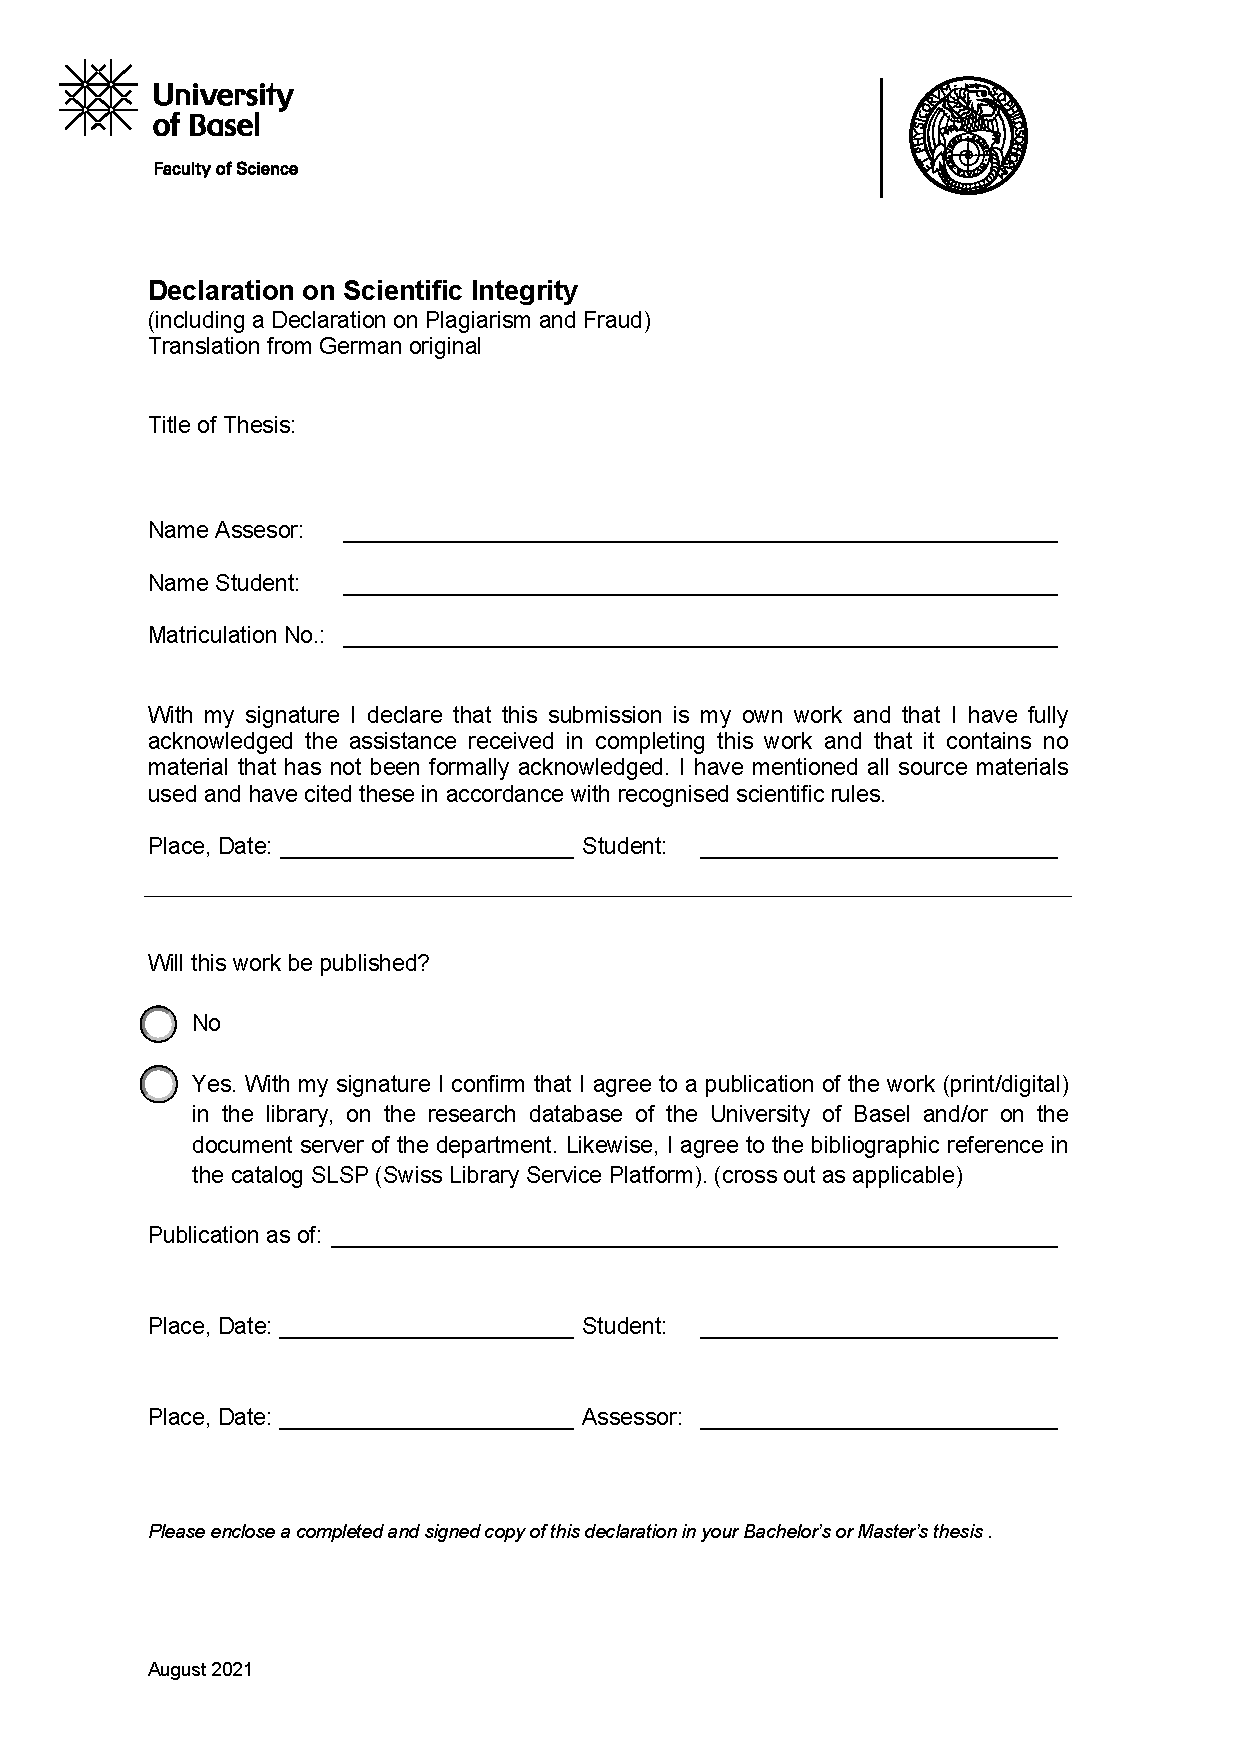
\includepdf{./Back/wissensch_Redlichkeit_E_Aug_21.pdf}}
  {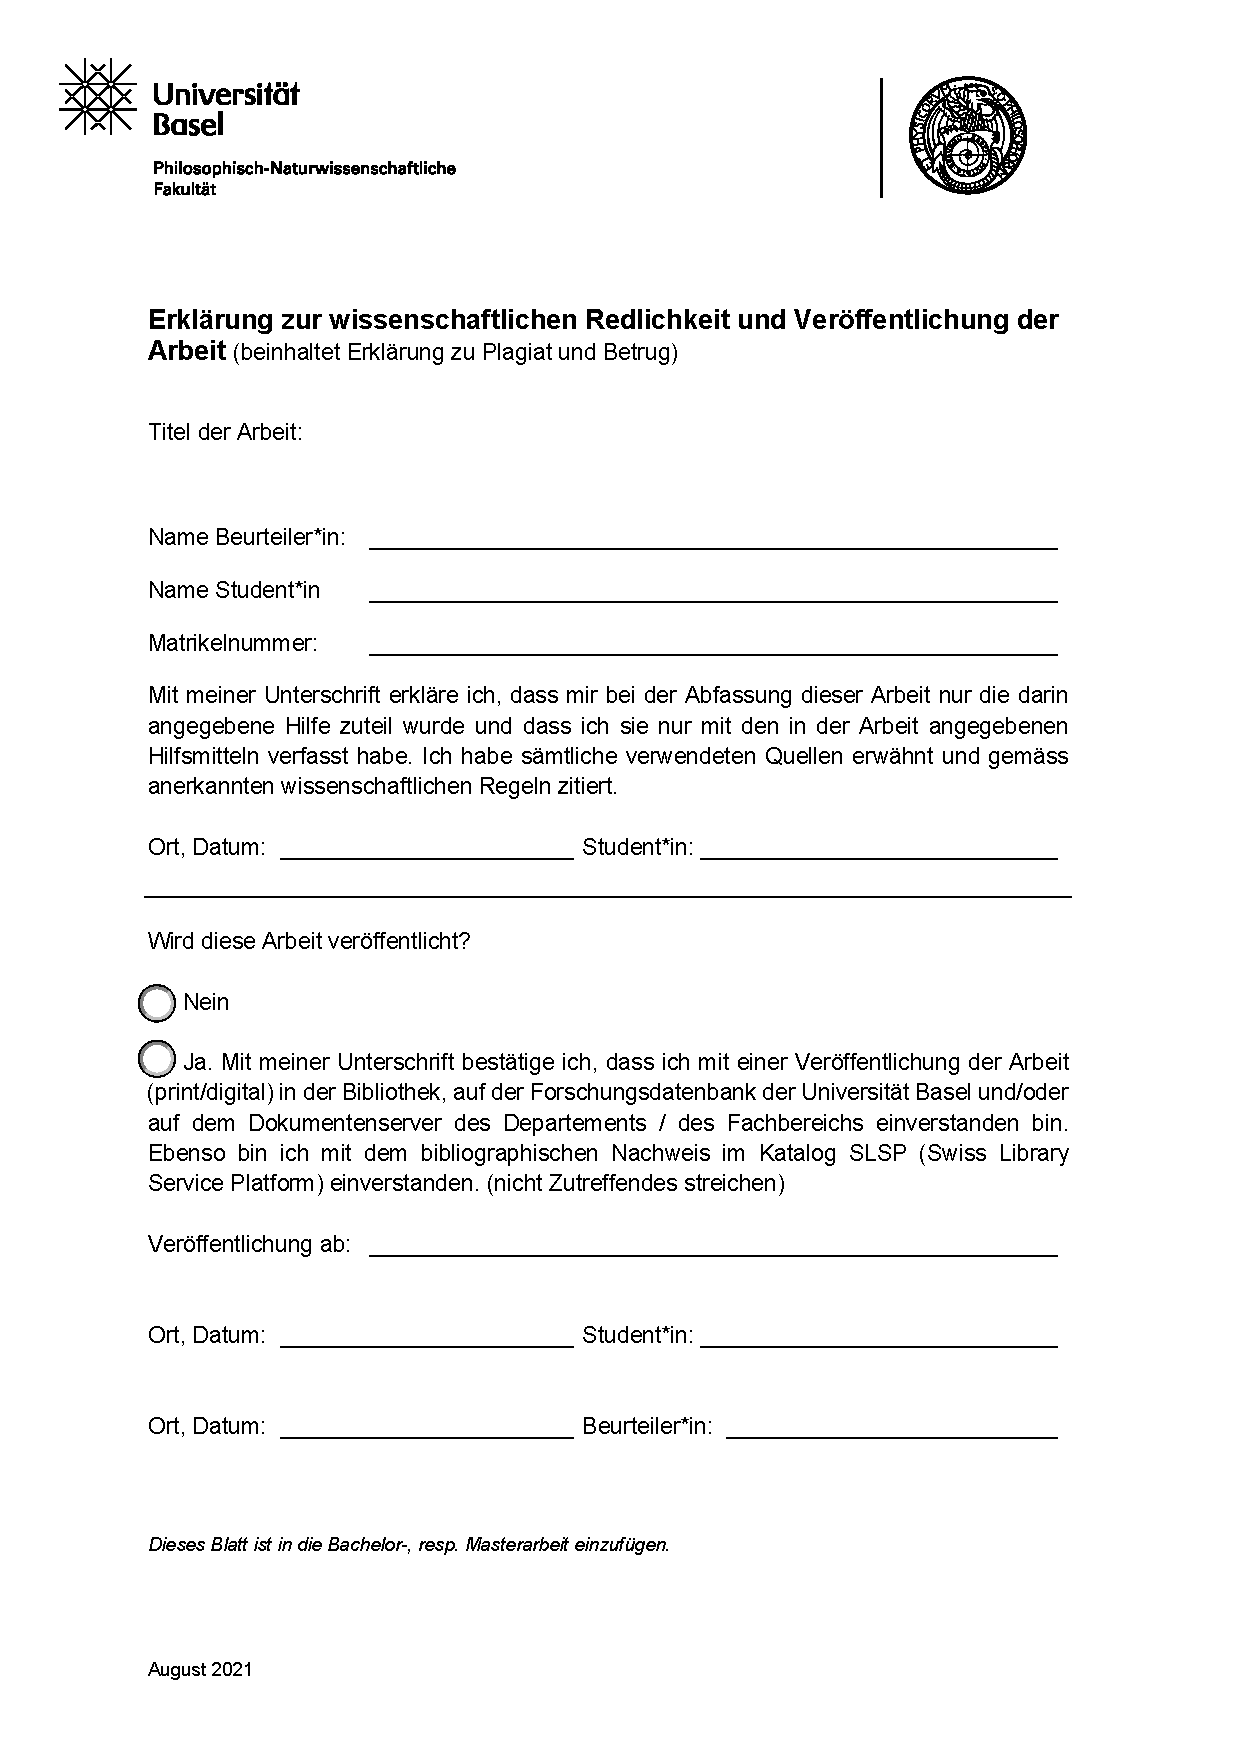
\includepdf{./Back/wissensch_Redlichkeit_D_Aug_21.pdf}}
%% ----------------------------------------------------------------
\end{document}
%% ----------------------------------------------------------------
